\documentclass[UTF8,12pt]{ctexart}
\usepackage{amsmath,amssymb,geometry,bm,graphicx,fontspec,amssymb,amsthm}
\usepackage[mathscr]{euscript}

\usepackage{tabularray}

\usepackage[colorlinks,
linkcolor=black,
anchorcolor=blue,
citecolor=green
]{hyperref} % 目录中的超链接

\newtheorem{Def}{定义}[section]
\newtheorem{Theo}{定理}[section]
\newtheorem{Lemm}{引理}[section]
\newtheorem{Prop}{命题}[section]
\newtheorem{Assu}{假设}[section]
\newtheorem{Axiom}{Axiom}

\numberwithin{equation}{section} % 按章节进行排序与编号
\numberwithin{figure}{section}
\numberwithin{table}{section}

\usepackage{draftwatermark} % 所有页加水印
\SetWatermarkText{EconNerd} % 设置水印内容
\SetWatermarkLightness{0.99} % 设置水印透明度 0-1
\SetWatermarkScale{1} % 设置水印大小    

\title{传播学} % 文档相关信息
\author{EconNerd}
\date{\today}
\geometry{scale=0.8}

\begin{document}
	\maketitle
	\tableofcontents
	\newpage
	
	\section{序言}
	本文的内容大部分来源于郭庆光的《传播学教程》,根据我的兴趣进行了取舍。
	
	整体文章章节仍然保持了原书的结构。总共包含12章。除去第一章的序言以及最后一张对于重要实验和理论的整理,整体可以分为三个部分。
	
	第一部分可以看作是总结介绍,为2-6章主要包含了对于传播学这个学科的介绍,发展历史,以及对于传播过程最基本的范式。其中最重要是拉斯韦尔的5W模式,以及他所形成的大众传播学研究的五大领域即“控制研究”、“内容分析”、“媒介分析”、“受众分析”和“效果分析”。
	
	第二部分主要包含7-11章。主要针对五大领域进行展开。主要关于控制研究、媒介分析、受众分析和效果分析
	
	第三部分包含12章,主要内容为传播学的研究史
	
	\newpage
	
	\section{传播学的基本介绍与历史发展}
	\subsection{基本介绍}
	第一章一如既往是介绍这个学科最基本的信息,例如从哪里来,研究什么问题。
	
	传播学最早的起源,有两个
	\begin{enumerate}
		\item (社会学起源)库利1909年《社会组织》中《传播》一章,定义\textbf{传播}指的是人与人的关系赖以成立和发展的机制——包括一切精神象征及其在空间中得到传递,在时间上得到保存的手段。它包括表情、态度和动作、声调、语言、文章、印刷品、铁路、电报、电话以及人类征服空间和时间的其他任何最新成果。
		
		\item (符号学起源)皮尔士1911年《思想的法则》中《传播》短章,定义直接传播某种观念的唯一手段是像(icon)。即使传播最简单的观念也必须使用像。因此,一切观点都必须包含像或像的集合,或者说是由表明意义的符号构成的。
	\end{enumerate}
	
	从20世纪40年代信息科学诞生以后,许多传播学家在界定传播概念之际都突出强调传播的信息属性。例如,著名传播学家施拉姆在《传播是怎样运行的》一文中写道:当我们从事传播的时候,也就是在试图与其他人共享信息——某个观点或某个态度……传播至少有三个要素:\textbf{信源、讯息和信宿}。
	
	关于通过研究的问题来定义一种学科。这是一种方法,但是并不是最有效以及常见的方法,因为我们不会在遇到一个问题先去问一下这是属于什么学科的问题。
	
	\subsection{人类传播的历史与发展}
	传播媒介也不断发展,哈特把有史以来的传播媒介分为三类:示现媒介、再现媒介、机器媒介
	
	\begin{enumerate}
		\item 示现的媒介系统。即人们面对面传递信息的媒介,主要指人类的口语,也包括表情、动作、眼神等非语言符号,它们是由人体的感官或器官本身来执行功能的媒介系统。
		
		\item 再现的媒介系统。包括绘画、文字、印刷和摄影等。在这一类系统中,对信息的生产和传播者来说需要使用物质工具或机器,但对信息接收者来说则不需要。
		
		\item 机器媒介系统。包括电信、电话、唱片、电影、广播、电视、计算机通信等。这些媒介,不但传播一方需要使用机器,接收一方也必须使用机器。
	\end{enumerate}
	
	\begin{figure}[h]
		\centering
		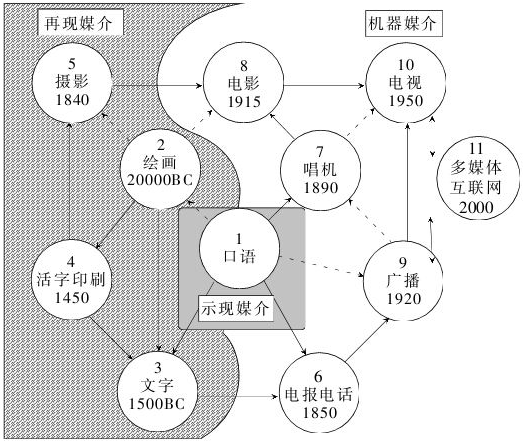
\includegraphics[width=0.7\linewidth]{history}
		\caption{}
		\label{fig:history}
	\end{figure}
	
	\newpage

	\section{人类传播的过程与系统结构}
	基于信源、讯息和信宿,我们可以把传播过程扩展为以下几个要素
	\begin{enumerate}
		\item 传播者。又称信源,指的是传播行为的引发者,即以发出讯息的方式主动作用于他人的人。在社会传播中,传播者既可以是个人,也可以是群体或组织。
		
		\item 受传者。又称信宿,即讯息的接收者和反应者,传播者的作用对象。作用对象一词并不意味着受传者是一种完全被动的存在,相反,他可以通过反馈活动来影响传播者。受传者同样可以是个人,也可以是群体或组织。
		
		受传者和传播者并不是固定不变的角色,在一般传播过程中,这两者能够发生角色的转换或交替。一个人在发出讯息时是传播者,而在接收讯息时则又在扮演受传者的角色。
		
		\item 讯息。讯息指的是由一组相互关联的有意义的符号组成,能够表达某种完整意义的信息。讯息是传播者和受传者之间社会互动的介质,通过讯息,两者之间发生意义的交换,达到互动的目的。
		
		讯息(message)一词,在中文里也译成“消息”、“文告”等,这是一个与信息(information)意思相近又有微妙区别的概念。一般来说,信息的外延更广,它包括讯息在内。讯息也是一种信息,其特点是能表达完整的意义。例如,甲向乙发电报希望乙马上回来,由于差错在电文中只写了一个“速”字。这个“速”字可以是一个信息,但不是讯息,只有“速归”才能构成一条讯息。在传播过程研究中,学者们通常使用“讯息”的概念,是为了强调社会传播的互动是意义完整的互动。
		
		\item 媒介。又称传播渠道、信道、手段或工具。媒介是讯息的搬运者,也是将传播过程中的各种因素相互连接起来的纽带。现实生活中的媒介是多种多样的,邮政系统、大众传播系统、互联网络系统、有线和无线电话系统都是现代人常用的媒介。
		
		\item 反馈。指受传者对接收到的讯息的反应或回应,也是受传者对传播者的反作用。获得反馈讯息是传播者的意图和目的,发出反馈讯息是受传者能动性的体现。反馈是体现社会传播的双向性和互动性的重要机制,其速度和质量因媒介渠道的性质而有不同,但它总是传播过程中不可或缺的要素。
	\end{enumerate}
	
	在传播学研究史上,不少学者采用建构模式的方法,对传播过程的结构和性质做了各种各样的说明。
	
	\subsection{直线模式}
		
	拉斯韦尔。1948年,他在一篇题为《传播在社会中的结构与功能》提出的5W模式,Who、Says what、In which channel、To whom、With what effect。\textbf{后来大众传播学研究的五大领域即“控制研究”、“内容分析”、“媒介分析”、“受众分析”和“效果分析”,就是沿着“5W”模式的这条思路形成的。}
	
	1949年香农和韦弗在《传播的数学理论》一文中也提出了一个过程模式,称为传播过程的数学模式或香农-韦弗模式。香农—韦弗模式是描述电子通信过程的。它的第一个环节是信源,由信源发出讯息,再由发射器将讯息转为可以传送的信号,经过传输,由接收器把接收到的信号还原为讯息,将之传递给信宿。在这个过程中,讯息可能受到噪音的干扰,产生某些衰减或失真。
	
	\subsection{循环模式和互动模式}
	
	1954施拉姆在《传播是怎样运行的》一文中,在CE.奥斯古德的观点启发的基础上,提出了一个新的过程模式,称为“循环模式”。此外施拉姆来针对大众传播提出了“大众传播过程模式”
	
	德弗勒的互动过程模式是在香农—韦弗模式的基础上发展而来的,它克服了前者单向直线的缺点,明确补充了反馈的要素、环节和渠道,使传播过程更符合人类传播互动的特点。
	
	
	\subsection{社会传播的系统结构}
	
	1959年,美国一对从事社会学研究的夫妇J.W.赖利和M.W.赖利在《大众传播与社会系统》一文中,提出了一个引人注目的传播系统模式
	
	德国学者马莱兹克于1963年在《大众传播心理学》一书中提出的系统模式
	
	社会传播的总过程
	
	\newpage
	
	\section{人内传播与人际传播}
	
	从社会信息系统微观、中观和宏观来看,分别有着不同的传播系统
	\begin{enumerate}
		\item 微观层面就是人内传播和人际传播
		
		\item 中观层面就是群体传播和组织传播
		
		\item 宏观层面就是大众传播
	\end{enumerate}
	
	
	
	
	
	\subsection{人内传播}
	人内传播(intra-personal communication),也称内向传播、内在传播或自我传播,指的是个人接受外部信息并在人体内部进行信息处理的活动。
	
	在人内传播是否有互动性方面,不同学者持有相反的观点。人内传播不但具有鲜明的社会性,而且具有明确的互动机制。考察人的自我意识是分析任内传播的重点。\textbf{这里有三种理论}
	
	\subsubsection{象征互动理论}
	最早从传播的角度对人的自我意识及其形成过程进行了系统研究的是美国社会心理学家G.H.米德(注:G.H.米德(1863—1931),美国社会心理学家,象征互动理论的创始人,从传播和社会互动的角度考察人的自我意识的形成过程。其主要论著收于逝世后出版的《心灵、自我与社会》(1934)一书中。)。米德在研究人的内省活动时发现,自我意识对人的行为决策有着重要的影响。自我可以分解成相互联系、相互作用的两个方面:一方是作为意愿和行为主体的“主我”(I),它通过个人围绕对象事物从事的行为和反应具体体现出来;另一方是作为他人的社会评价和社会期待之代表的“客我”(me),它是自我意识的社会关系性的体现。
	
	现代象征互动理论的集大成者H.布鲁默(注:H.布鲁默(1900—1987),美国社会心理学家,象征互动理论的集大成者,代表性著作有《象征互动论》(1969)等。)的“自我互动”理论也是对人内传播的社会性和互动性的一个很好说明。
	
	\subsubsection{内省}
	内省是人对自己的一种反思活动,也是一种重要的人内传播形式。内省可以分为两种,一种是日常的、长期的自我反思活动,它以完善个人的品德和行为为目的,具有明显的长期目标性和连贯性。在我国的儒家思想中,内省主要指的是人的自我修养,曾子的“吾日三省吾身”、孔子的“内省不疚,夫何忧何惧”等论述,都是这个意思。另一种是短期的、以解决现实问题为目的的自我反思活动,称为“内省式思考”(reflective thinking)。在这里,我们主要考察后者,并由此来探讨人内传播在社会实践中所起的作用。
	
	\subsubsection{基模}
	古往今来,每个人都需要快速有效地处理信息,特别是在信息爆炸的当今时代,这种必要性更为突出。但是,我们也发现,尽管海量信息扑面而来,但我们每个人在应对和处理上却能做到有条不紊,从容不迫。那么,究竟是什么机制在发挥作用呢?对此,认知心理学提供了一种说明:我们之所以能够快速有效地认知、分析和判断新信息或新事物,是因为在我们的大脑中有一种被称为“认知基模”(cognitive schema)的东西在起作用。
	
	基模作为我们的大脑中预存的认知结构,影响我们每个人信息处理的全过程及其结果。1973年,美国学者罗伯特·阿克塞尔罗德在他的《认知与信息处理过程的基模理论》一文中,提出了一个信息处理过程模式。
	
	这个理论认为,每个人都会以两种不同方式处理信息,一种是以详尽的方式,用严谨的思考来处理信息,另一种是以较为简单粗略的方式来处理信息;前者是沿“核心路径”(central route)处理信息,后者则是沿“边缘路径”(peripheral route)处理信息。
	
	\subsection{人际传播}
	人际传播是个人与个人之间的信息传播活动,也是由两个个体系统相互连接组成的新的信息传播系统。人际传播是一种最典型的社会传播活动,也是人与人社会关系的直接体现。
	
	自我意识是在与他人的社会交往和传播中形成的——我们在本章中介绍米德和布鲁默等人的理论时已经对这个问题做了阐述。在这里,我们与人际传播的动机相联系,再补充介绍一下美国社会学家C.H·库利(注:C.H.库利(1864—1929),美国社会学家,对传播与人的社会化问题进行了深研究,并提出了“初级群体”和“镜中我”概念。主要著作有《人类本性与社会秩序》(1902)、《社会组织》(1909)等。)的“镜中我”(the looking-glass self)概念。
	
	库利是在1909年出版的《社会组织》一书中提出“镜中我”概念的。他认为,人的行为在很大程度上取决于对自我的认识,而这种认识主要是通过与他人的社会互动形成的,他人对自己的评价、态度等,是反映自我的一面“镜子”,个人透过这面“镜子”认识和把握自己。因此,人的自我是在与他人的联系中形成的,这种联系包括三个方面:
	\begin{enumerate}
		\item 关于他人如何“认识”自己的想象。
		
		\item 关于他人如何“评价”自己的想象。
		
		\item 自己对他人的这些“认识”或“评价”的情感。
	\end{enumerate}
	
	个人从事人际传播的重要动机之一是自我认知和相互认知。相互认知的一个重要方面是希望对方能够充分地了解、理解和评价自己。然而,对方能不能做到这一点,在很大程度上取决于自己的自我表达是否充分。人际传播,对双方来说都是一种自我表达活动。所谓自我表达,即传播者“将自己的心情、意志、感情、意见、态度、考虑以及地位、身份等等向他人加以表达的活动”(注:[日]船津卫:《传播学入门》,1版,58页,东京,有斐阁,1997。)。自我表达是否准确,表达方式是否合适,直接影响人际传播的效果。
	
	\newpage
	
	\section{群体传播、集合行为、组织传播}
	分析中观的传播系统,首先要定义什么是群体以及什么是组织
	
	\subsection{群体传播}
	群体的含义是十分广泛的。日本社会学家岩原勉认为,所谓群体,指的是“具有特定的共同目标和共同归属感、存在着互动关系的复数个人的集合体”(注:[日]见田宗介等:《社会学事典》,1版,439页,东京,弘文堂,1988。)。
	
	岩原勉认为,群体的本质特征有两个:
	\begin{enumerate}
		\item 目标取向具有共同性。这就是说,参与群体活动的个人都是带着某种共同的目的——共同的利益、关注点、兴趣等而集合到一起的。
		
		\item 具有以“我们”意识为代表的主体共同性,如日常生活中经常听到的“我们消费者”、“我们青年人”、“我们工薪阶层”等,“我们”体现了一种主体共同性。这两个特征意味着任何一个群体都具有互动机制和使共同性得到保障的机制,这种机制称为群体的组织性。
		
	\end{enumerate}
	
	不同学者对群体的分类是不同的。美国社会学家库利根据群体在个人社会化过程中所起作用的直接和间接程度,将群体分为初级群体(primary group)和次级群体(secondary group)。德国社会学家M.韦伯将群体中是否存在管理主体或机构作为分类标准,把拥有管理组织系统的群体称为“团体”(verband),其他则属于一般群体。另一位德国社会学家L威瑟也依据组织性的强弱,将群体分成两类,一类是组织群体(organization),另一类是非组织群体。
	
	在群体的分类中,有特殊的一类。就是临时的集合行为(collective behavior)所产生的聚集的人群,法国社会心理学家勒朋称之为“乌合之众”(crowd)。集合行为所产生的人群,与我们通常所讲的一般社会群体或组织群体有不同的性质,需要作为一种独特的群体现象加以考察。

	
	群体具有重要的社会功能,这种功能,简言之即群体是将个人与社会相联结的桥梁和中间纽带。群体是社会的中观系统,是社会的组成部分,或者说是“局部社会”。
	
	群体的成立、生存和发展需要一些条件,其中最基础的条件有三项:(1)共同的目标和关心事项,这是群体凝聚力的核心;(2)成员之间的协作意愿,也就是个人参加群体并愿意为之做出贡献的动机;(3)群体与成员、成员与成员间的传播互动机制,即群体传播。岩原勉认为:“群体传播就是将共同目标和协作意愿加以连接和实现的过程。”(注:[日]见田宗介等:《社会学事典》,1版,440页,东京,弘文堂,1988。)
	
	群体传播在群体意识的形成中起着重要的作用。所谓群体意识,就是参加群体的成员所共有的意识。它包括以下几个方面的内容:(1)关于群体目标和群体规范的合意;(2)群体感情,这里不仅指由各成员的密切接触和协作而产生的成员间的个人感情,更指群体成员主观境界的融合(精神上的一体化)所产生的“我们”感情;(3)群体归属意识,即群体成员因从群体活动得到某种程度的需求满足而对群体所产生的认同感。这几个要素越具备,群体意识就越强,越欠缺则群体意识越薄弱。
	
	群体传播形成群体意识,这种意识一旦形成,也会对群体传播产生重要的影响。群体意识的影响主要体现在对成员个人的态度和行为的制约作用上。法国社会学家E.迪尔凯姆(注:E.迪尔凯姆(1858—1917),又译涂尔干,法国社会学家。主要著作有《社会分工论》(1893)、《社会学方法的基准》(1895)和《社会学与哲学》(1924)等。)认为,群体意识虽然可以通过社会化过程为个人所吸收,但总体上仍然属于一种集合意识,是相对于个人意识的一种外在的、约束性的思维、感情和行为方式。
	
	群体意识的核心内容是群体规范。群体规范指的是成员个人在群体活动中必须遵守的规则,在广义上也包括群体价值,即群体成员关于是非好坏的判断标准。一般认为,群体规范的功能包括以下几项:(1)协调成员的活动、规定成员角色和职责以促进群体目标的达成;(2)通过规范的共有来保证群体的整体合作;(3)通过指示共同的行为方式以维持群体的自我同一性(identity);(4)为成员个人提供安全的决策依据。
	
	在群体传播中,群体规范的主要作用在于排除偏离性的意见,将群体内的意见分歧和争论限制在一定范围之内,以保证群体决策和群体活动的效率。每个群体都有一般成员承认并且拥护的规范体系,成员个人的群体归属意识越强,也就越倾向于积极维护群体规范。群体规范的维持通过群体内的奖惩机制来保证。在成员个人对群体做出了贡献的时候,可以得到群体的奖励,包括获得其他成员的赞扬和在群体内角色地位的上升等;当从事了不利于群体或违背群体规范的行为之际,个人成员将会受到群体的制裁,包括受到其他成员的冷遇而陷于孤立状态、各种不同程度的处分直至被排除于群体之外。因此,当个人的态度和行为与群体规范发生冲突时,他所面临的群体压力是巨大的。
	
	在群体内部,传播活动经常是在“一对多”或“多对一”、“少数对多数”或“多数对少数”的场合下进行的。在这种情况下,无论是传播者还是受传者都会感受到某种程度的群体压力。所谓群体压力,即群体中的多数意见对成员中的个人意见或少数意见所产生的压力。在面临群体压力的情况下,个人和少数意见一般会对多数意见采取服从态度。
	
	\paragraph{趋同心理}
	
	“个人服从集体、少数服从多数”是群体活动的一个基本原则。它不仅是群体保持协调统一的前提,也是人的社会合作性的体现。德国传播学者伊丽莎白·诺尔诺依曼认为,能否顺应多数意见,是对一个人的道德规范和基本价值与社会是否相容的一种“检验”。(注:See Elizabeth Noelle-Neumann,The Spiral of Silence,Chicago \&London,The University of Chicago Press,1984,p.72.)这就是说,人为了进行有效的社会合作,需要对多数人的意见做出一定程度的妥协和让步,极端个人主义是不符合社会道德的。然而,对多数意见的服从决定并不是在任何情况下都是基于理性判断做出的。在不少场合,群体压力也会带来错误的判断,形成对多数意见的盲目服从。美国心理学家所罗门·阿什在20世纪50年代进行的小群体内趋同行为实验充分证明了这一点。
	
	当然,多数意见的支配地位并非在任何场合都是绝对的。另一位心理学家S.莫斯考维西的同类实验也证明,群体中少数意见的中坚人物(hard core)的作用也是不可忽视的。当这些中坚人物显示出意志的坚定性、主张的一贯性和态度表明的强烈性之际,可以对多数派产生有力的影响,甚至可以改变群体已有的合意并形成新的合意。(注:参见[日]小关八重子:《少数派的影响过程》,见《社会心理学视点》,东京,诚信书房,1988。)这说明在群体传播活动中,还有另一种并不基于群体压力和趋同心理的合意形成机制。
	
	\subsection{集合行为}
	集合行为(collective behavior),指的是在某种刺激条件下发生的非常态社会聚集现象。例如火灾、地震后的群众骚乱,出于某种原因的自发集会、游行、种族冲突,物价上涨的流言引起的抢购风潮等。集合行为多以群集、恐慌、流言、骚动的形态出现,往往会造成对正常的社会秩序的干扰和破坏。
	
	关于集合行为是否属于群体行为,在学界有各种不同的观点。有的学者认为群体至少应具有某种程度的组织性,而集合行为完全是自发的和无组织的,因而否认它是群体行为。也有的学者认为,集合行为是以一种非常态的群体——群集(crowd)的形式进行的,群集虽然与一般社会群体有着明显不同,但就其内部存在着参加者个人之间、参加者个人与人群全体之间的互动关系而言,群集也应该属于广义的群体的范畴。我们在这里取后一种观点,即把集合行为看做一种非常态的群体行为,把集合行为中的传播看做非常态的群体传播。
	
	集合行为虽然是一种自发的反常现象,但它的产生是有条件的。一般认为,集合现象的发生需要三个基本条件:
	\begin{enumerate}
		\item 结构性压力
		
		\item 触发性事件
		
		\item 正常的社会传播系统功能减弱,非常态的传播机制活跃化。
	\end{enumerate}
	
	
	集合行为中的信息传播,与正常的社会传播有很大的不同,它受到一些特殊传播机制的制约。
	\begin{enumerate}
		\item 群体暗示与群体感染
		
		集合行为中的传播可以分为两个方面,一是信息本身的传播,二是与此相伴随的情绪或感情的传播,这两种传播都摆脱不了暗示与感染机制的支配。暗示指的是一种传播方式,即不是通过直接的说服或强制,而是通过间接的示意使人接受某种观点或从事某种行为。
		
		暗示在人际传播当中也是常见的,但在这里,接不接受暗示通常基于受传者的理性判断。而集合行为中的暗示则不同,它更接近于临床医学中的催眠暗示。也就是说,集合行为通常是大量人群聚集于狭小的物理空间,人们保持着高密度的接触,参加者通常处于亢奋、激动的精神状态,这样一些情境状态容易使他对周围的信息失去理智的分析批判能力,表现为一味的盲信和盲从。法国社会心理学家勒朋(注:勒朋(1841—1931),法国社会心理学家,以研究集合心理著名。主要著作有《群众心理》(1895)等。)认为,处于激动的人群中的个人具有很强的“被暗示性”,周围人的话语、表情、动作乃至现场的氛围,对他都成为有力的暗示刺激,使他的信念、思维和行为方式迅速与现场的人群融为一体。
		
		与群体暗示相联系的另一种机制是群体感染。在集合行为中,群体感染指的是某种观念、情绪或行为在暗示机制的作用下以异常的速度在人群中蔓延开来的过程。其传播的速度快,主要原因还是由于在现场亢奋的氛围中,成员失去理性的自控能力,而对来自外部的刺激表现出一种本能的反应,如一人大哭,全场便跟着大哭;一人大笑,全场跟着大笑等。经过这种群体感染过程,一种情绪、一种观点会迅速支配整个人群,并迅速引发整个人群的激烈行动。
		
		\item 群体模仿与“匿名性”
		
		群体模仿是解释集合行为中的传播机制的另一种理论。模仿是法国社会心理学家塔尔德(注:J.G.塔尔德(1843—1904),法国社会心理学家,“公众”概念的提出者,主要著作有《模仿律》(1890)、《舆论与群众》(1901)等。)提出的概念,他在1890年出版的《模仿律》一书中认为,社会上的一切事物不是发明就是模仿,而“模仿是最基本的社会现象”。模仿又分为无意识模仿和有意识模仿,前者是个人在不自觉状态下对他人行为的反射性仿效,而后者则是基于一定动机或目的的自觉仿效。人在社会化过程中的各种学习,也可以说是一种自觉的模仿或有意识模仿。
		
	\end{enumerate}
	
	流言(rumor)是自古以来社会生活中常见的信息传播现象,也是人们在价值判断上有着分歧和争议的一种现象。一方面,人们把流言看做正式渠道信息的补充,而现实生活中,流言或小道消息最后证实为事实的事例并不少见。另一方面,流言由于其暧昧性和不可靠性,不容易与别有用心的谣言相区别,同时又常常引起不良社会后果,故而人们对流言的评价一般是负面的。
	
	美国心理学家奥尔波特与波斯特曼曾经为流言下过这样一个定义:所谓流言,是“一种通常以口头形式在人们中间流传,涉及人们信念而目前没有可靠证明标准的一种特殊的陈述或话题”(注:参见奥尔波特、波斯特曼等:《谣言心理学》,序,第2页,沈阳,辽宁教育出版社,2003。)
	
	对此,奥尔波特首先提出了一个著名的流言流通量公式,他认为,在一个社会中,“流言的流通量,与问题的重要性(importance)和涉及该问题的证据暧昧性(ambiguity)之乘积成正比”(注:G.W.Allport,The Psychology of Rumor,New York,Henry Holt,1947,pp.133-135.)。这句话改写成公式即:
	
	R=I×A (流言流通量=问题的重要性×证据的暧昧性)
	
	奥尔波特的这个公式指出了流言发生的两个特点:第一,流言通常是围绕人们关心的问题、涉及切身利益的重要问题发生的;第二,来自正式渠道的有证据的信息(如大众传播媒介的报道、权威部门的信息发布等)不足、状况的暧昧性、不确定性增加,会推动人们去通过流言渠道寻求信息。换句话说,涉及的问题越重要,真相越是含糊不清,流言传播活跃的几率越大。
	
	在后来的研究中,研究人员发现上述两个变量还不足以更精准地阐释流言传播的条件,又对该公式做了进一步的修正。如印度心理学家巴萨德早在1934年对地震流言的研究中就发现“不安感”(anxiety)是流言发生和传播的重要推动力,而美国学者苏姗·安索尼1973年对高中生的试验结果也证明了“不安程度高的人更倾向于传播流言”的结论,并且得到了其他学者同类研究的肯定。另外,奥尔波特公式的另外两个变量——“重要性”(importance)和“暧昧性”(ambiguity),也为“关联度”(involvement)和“不确定性”(uncertainty)所代替。(注:参见蔡静:《流言:阴影中的社会传播》,20~24页,北京,中国广播电视出版社,2008。)
	
	因此,目前考察流言的发生与传播通常采用下述公式:
	
	R=I×A×U(流言流通量=与问题的关联度×社会成员的不安感×环境的不确定性)
	
	在这里,“关联度”指的是社会成员与流言信息所涉及问题的关联程度,人们与该问题关系越密切,越有卷入流言传播的可能,而且在通常情况下,流言是从关系最密切的群体中滋生和蔓延开来的。“不安感”强调的是流言发生和传播的心理条件,其中包含对事件未来发展的解释或忧惧。“不确定性”既是指环境的不稳定状态,也是指由于权威信息渠道不畅通或公信力缺失所导致的信息紊乱。
	
	流言是集合行为中的主要信息形态。流言可分为非紧急事态下的流言和紧急事态下的流言,集合行为中的流言则属于紧急事态下的流言。在集合行为中,信息的流动也呈现出一种异常状态,在这里,要辨认谁是信源、谁是信宿是十分困难的,几乎每个人都是消息的发布者,同时也是消息的接受者。美国社会学家H.布鲁默认为,集合行为的初步形态是“循环反应”。所谓循环反应,即一方的刺激成为另一方的反应,而另一方的反应又反过来成为这一方的刺激的循环往复过程。
	
	集合行为中的“信息流”有如下几个特异点:
	\begin{enumerate}
		\item 流言信息的快速增殖
		
		\item 流言信息的变形和奇异回流现象
		
		\item 流言中伴随着大量的谣言。谣言(lie)不同于流言(rumor)。流言有自然发生的,也有人为制造的,但大多与一定的事实背景相联系;而谣言则是有意凭空捏造的消息或信息。
	\end{enumerate}
	
	
	\subsection{组织传播}
	与非组织群体不同的是,组织是一个结构秩序更为严密的社会结合体,有着更为明确的目标、制度、纪律,有着严格的分工和统一的指挥管理体系,因此,组织是人们为了高效率地完成分散的个人或松散的群体所不能承担的生产或社会活动而结成的协作体。作为组织的基本属性之一的组织传播,同样体现了它的这些特点。现代社会是高度组织化的社会,也是组织传播高度发达的社会。
	
	什么是组织从广义上来说,任何由若干不同功能的要素按照一定的原理或秩序相组合而形成的统一整体,都可以称为组织,如细胞组织、肌肉组织、人体组织等。在狭义上,组织指的是“人们为实现共同目标而各自承担不同的角色分工,在统一的意志之下从事协作行为的持续性体系”(注:[日]见田宗介等:《社会学事典》,1版,556页,东京,弘文堂,1988。)。
	
	一般来说,辨认一个群体是否属于组织,主要看这个群体中是否有一个统一的指挥或管理系统,用马克斯·韦伯的话来说,即是否存在着一个“管理主体”。在这个分类标准下,凡是具有中枢指挥或管理系统的群体,如政党、军队、政府机构、企业、社团等,都属于组织的范畴。
	
	组织都是为了实现一定的组织目标而设置或成立的。因此一般有着如下的特征
	\begin{enumerate}
		\item 专业化的部门分工
		
		\item 职务分工和岗位责任制
		
		\item 组织系统的阶层制或等级制
	\end{enumerate}
	
	组织传播究竟是一种什么性质的传播?不少学者对这个问题的回答都是比较模糊的。美国人戈德哈伯曾经为它下过一个定义:“组织传播系由各种相互依赖关系结成的网络,为应付环境的不确定性而创造和交流信息的活动。”(注:范东生、张雅宾:《传播学原理》,1版,256页,北京,北京出版社,1990。)
	
	这个简单的解答就是:所谓组织传播,就是以组织为主体的信息传播活动。组织传播既然是人类传播的一种类型,就必然会有与其他类型传播相通的共性;而它又是以组织为主体的传播,这就决定了它具有与其他类型所不同的特点。美国学者凯瑟琳·米勒在《组织传播》一书中也指出:“组织传播涉及两个复杂的概念的结合——组织和传播,两者都有多种多样的界定和多种视角的考察,因此很明显,没有唯一正确的定义。”(注:K.Miller,Organizational Communication:Approaches and Processes,ThirdEdition,Wadsworth,2003,p.1.)
	
	组织内传播有着正式渠道和非正式渠道。正式渠道包括了
	\begin{enumerate}
		\item 下行传播
		
		\item 上行传播
		
		\item 横向传播
	\end{enumerate}
	
	非正式渠道主要有两种形式:一是组织内的人际传播,如组织成员工作之余的交谈、单位内外的各种私人交往等;二是非正式的小群体传播,如各种自发的革新小组、兴趣小组或联谊会中的信息交流等。
	
	正式渠道中的传播体现了组织成员作为“组织人”的特点,而非正式渠道中的传播则体现了他们作为“社会人”的特点。对一个组织来说,能否充分发挥非正式传播渠道的作用具有重要的意义。传统的组成管理理论往往只关注机构分工、职权划分、规章制度的作用,在这种理论指导下,人往往被“异化”为组织这部机器上的一个零部件。与此相比,自“霍桑实验”(注:霍桑实验:1924年至1932年美国在芝加哥西方电器公司的霍桑工厂进行的企业管理改革实验,以1927年哈佛大学教授梅奥主持的心理学实验最为有名,该研究强调了心理和社会因素对劳动态度和生产效率的影响。)
	
	
	除了组织内部的信息传播还有组织和外部环境的信息交互也是重要的研究范围。其中主要包括了组织的信息输入和组织的信息输出。
	
	输出的活动中主要包含了三种
	\begin{enumerate}
		\item 公关宣传
		
		“公关”是公共关系的简称,是英语public relations的对译词,通常缩写为PR。公共关系,指的是社会组织与周围社会环境中的其他组织、机构、团体以及公众的关系和联系;公关宣传,则是指组织为了与其所处的社会环境建立和保持和谐关系而进行的各种宣传活动。
		
		\item 广告宣传
		
		广告是一种以付费形式利用各种媒体进行的大面积宣传活动,也是社会组织尤其是企业组织广泛采用的一种信息输出方式。现代组织从事的广告活动大致可分成两类,一类是非商业广告,如公益广告、意见广告以及通过媒体发布的各种公告等;另一类是商业广告,以企业组织为主体。商业广告依其目的可分为企业形象广告和促销广告两种;以媒体而论,则可进一步分为报刊广告、影视广告、音声广告、现场促销广告(即POP,Point of Purchase的缩写)、屋外广告、交通广告、邮寄广告等等。
		
		\item 企业标识系统宣传
		
		企业标识系统是英语corporate identity system的对译词,简称CIS,有时也译为“企业表征系统”。CIS活动指的是企业组织使用统一的象征符号系统来塑造、保持或更新企业形象的活动,所采用的象征符号一般为具有特色的视觉图案(包括社名、社色等),它可以印制在社旗、社徽、制服、办公用具和各类产品及其包装上,以保持企业的视觉形象统一。社歌则是一种听觉标识。
	\end{enumerate}

	\newpage

	\section{大众传播}
	\subsection{大众传播的定义、特点与社会功能}
	关于什么是大众传播,学者们有各种各样的定义。这里试举几例:
	
	大众传播是“人类社会信息交流的方式之一,职业工作者(记者、编辑)通过机械媒介(印刷媒介、电子媒介)向社会公众公开地、定期传播各种信息的一种社会性信息交流活动”(注:刘建明主编:《宣传舆论学大辞典》,1版,290页,北京,经济日报出版社,1993。)。
	
	大众传播“指特定的社会集团通过文字(报纸、杂志、书籍)、电波(广播、电视)、电影等大众传播媒介,以图像、符号等形式,向不特定的多数人表达和传递信息的过程”(注:沙莲香:《传播学:以人为主体的图象世界之谜》,1版,145页,北京,中国人民大学出版社,1990。)。
	
	“大众传播即现代印刷和广播、电视等影像和声音媒介组织运用法人资金,借助高科技和产业化手段,在国家调控(state-regulated)的范围内向未知的受众提供信息和娱乐产品的实践活动。”(注:T.O'Sullivan,Key Concepts in Communication,New York,Methuen \&Co.,1985,p.130.)
	
	实际上,由于大众传播是一种极为复杂的社会现象,任何一个简短的定义都不可能概括它的全部特征。在这里,我们结合本教材的宗旨,对这一概念做出如下界定:所谓大众传播,就是专业化的媒介组织运用先进的传播技术和产业化手段,以社会上一般大众为对象而进行的大规模的信息生产和传播活动。
	
	大众传播有着如下的特点
	\begin{enumerate}
		\item 大众传播中的传播者是从事信息生产和传播的专业化媒介组织。
		
		\item 大众传播是运用先进的传播技术和产业化手段大量生产、复制和传播信息的活动
		
		\item 大众传播的对象是社会上的一般大众,用传播学术语来说即“受众”。
		
		\item 大众传播的信息既具有商品属性,又具有文化属性
		
		\item 传播过程的性质来看,大众传播特别是以报刊、广播、电视为代表的传统大众传播,属于单向性很强的传播活动。
		
		\item 大众传播是一种制度化的社会传播
	\end{enumerate}

	
	针对大众传播的功能,有着不同的代表性理论
	
	(一)拉斯韦尔的“三功能说”
	
	在传播学研究史上,最早对传播的社会功能做出较全面分析的是H拉斯韦尔。他在1948年发表的《传播在社会中的结构与功能》一文中,将传播的基本社会功能概括为以下三个方面:(注:See H.Lasswell,"The Structure and Function of Communication in Society",in Lyman Bryson(Eds),The Communication of Ideas,New York,Cooper Square ,1964,p.38.)
	\begin{enumerate}
		\item 环境监视功能(surveillance of the environment)
		
		自然与社会环境是不断变化的,只有及时监控、了解、把握并适应内外环境的变化,人类社会才能保证自己的生存和发展。在这个意义上,传播对社会起着一种“瞭望哨”的作用。
		
		\item 社会联系与协调功能(correlation of the parts of society)
		
		社会由各不同部分组成,是一个建立在分工合作基础上的有机体,只有实现了社会各组成部分之间的联络、协调和统一,才能有效地适应环境的变化。传播正是执行联络、沟通和协调社会关系功能的重要社会系统。
		
		\item 社会遗产传承功能(transmission of social heritage)
		
		人类社会的发展是建立在继承和创新的基础之上的,只有将前人的经验、智慧、知识加以记录、积累、保存并传给后代,后人才能在前人的基础上做进一步的完善、发展和创造。传播是保证社会遗产代代相传的重要机制。
		
		拉斯韦尔的上述观点被称为传播的“三功能说”。这三项功能是包括人际传播、群体传播、组织传播在内的一切社会传播活动的基本功能,大众传播不仅具备这些功能,而且起着突出重要的作用。
	\end{enumerate}
	
	
	
	(二)赖特的“四功能说”(注:[美]威尔伯·施拉姆等:《传播学概论》,32页。)
	
	美国学者C.R.赖特在《大众传播:功能的探讨》(1959)中,继承了拉斯韦尔“三功能说”,并在此基础上围绕大众传播的社会功能问题提出了“四功能说”:
	
	\begin{enumerate}
		\item 环境监视
		
		大众传播在特定社会的内部和外部收集和传达信息的活动。这里包括两个方面:一是警戒外来威胁,二是满足社会的常规性活动(政治、经济、生活)的信息需要。在这里,大众传媒的新闻报道起着尤其重要的作用。
		
		\item 解释与规定
		
		大众传播并不是单纯的“告知”活动,它所传达的信息中通常伴随着对事件的解释,并提示人们应该采取什么样的行为反应。新闻信息的选择、解释和评价将人们的视线集中于某些特定的事件,社论或评论也都是有明确意图的说服或动员活动。“解释与规定”的目的是为了向特定方向引导和协调社会成员的行为,其含义与拉斯韦尔的“社会协调”是一致的。
		
		\item 社会化功能
		
		大众传播在传播知识、价值以及行为规范方面具有重要的作用。现代人的社会化过程既是在家庭、学校等群体中进行的,也是在特定的大众传播环境中进行的。这个功能,与拉斯韦尔的“社会遗产传承”功能是相对应的,也有一些学者将之称为大众传播的教育功能。
		
		\item 提供娱乐
		
		大众传播中的内容并不都是务实的,其中相当一部分是为了满足人们的精神生活的需要,如文学的、艺术的、消遣性、游戏性的内容等。大众传播的一项重要功能是提供娱乐,尤其在电视媒体中,娱乐性内容占其传播的信息总量的一半以上。
		
	\end{enumerate}
	
	(三)施拉姆对大众传播社会功能的概括
	
	对拉斯韦尔和赖特的观点,施拉姆曾在1982年出版的《男人、女人、讯息和媒介》(中译本名为《传播学概论》)一书中,从政治功能、经济功能和一般社会功能三个方面进行了总结
	
	施拉姆把环境监视、社会联系协调和遗产传承归入政治功能的范畴,而把社会控制、规范传递、娱乐等归入一般社会功能的范畴。这种划分并没有明确的标准,也不见得十分确切。施拉姆分类法的重要贡献是明确地提出了传播的经济功能,指出了大众传播通过经济信息的收集、提供和解释,能够开创经济行为。施拉姆认为:“采用机械的媒介,尤其是电子媒介所成就的一件事,就是在世界上参与建立了史无前例的宏大的知识产业。”(注:[美]威尔伯·施拉姆等:《传播学概论》,155页。)这就是说,大众传播的经济功能并不仅仅限于为其他产业提供信息服务,它本身就是知识产业的重要组成部分,在整个社会经济中占有重要的地位。施拉姆的这个观点,已经为当代信息社会、知识经济和文化产业的发展所证实。
	
	(四)拉扎斯菲尔德和默顿的功能观
	
	关于大众传播的社会功能,还有一些学者从其他角度提出了另一些观点。例如,与拉斯维尔同时,拉扎斯菲尔德和默顿在1948年发表的《大众传播、通俗口味和有组织的社会行动》一文中,特别强调了大众传播的下述三种功能:(注:See P.Lazarsfeld \&R.K.Marton,"MassCommunication,Popular Taste and Organizational Action",in Lyman Bryson(Eds.),The Communication of Ideas,New York,Cooper Square ,1964.)
	
	\begin{enumerate}
		\item 社会地位赋予功能(status conferral)
		
		任何一种问题、意见、商品、团体乃至人物或社会活动,只要得到大众传媒的广泛报道,都会成为社会瞩目的焦点,获得很高的知名度和社会地位。拉扎斯菲尔德和默顿认为,这种地位赋予功能,会给大众传媒支持的事物带来一种正统化的效果。
		
		\item 社会规范强制功能(enforcement of social norms)
		
		大众传媒通过将偏离社会规范和公共道德的行为公之于世,能够唤起普遍的社会谴责,将违反者置于强大的社会压力之下,从而起到强制遵守社会规范的作用。拉扎斯菲尔德和默顿指出,大众传播的这项功能主要来自它的公开性。他们认为,在通常情况下,即使人们对违反规范的行为有所知晓,也不会发生有组织的社会制裁行动。但当大众传媒将问题公开化以后情况则不同,一般公众就会感受到维护社会规范的“制度性压力”,积极加入到舆论制裁的行列中去。
		
		\item 作为负面功能的“麻醉作用”(narcotizing dysfunction)
		
		拉扎斯菲尔德和默顿认为,现代大众传播具有明显的负面功能。它将现代人淹没在表层信息和通俗娱乐的滔滔洪水当中,人们每天在接触媒介上花费大量的时间和精力,降低了积极参与社会实践的热情:他们在读、在听、在看、在思考,但是,他们却把这些活动当做行动的代替物。他们有知识、有兴趣,也有关于今后的各种打算,但是,当他们吃完晚饭、听完广播、读完晚报以后,也就到了睡觉的时间了。拉扎斯菲尔德和默顿把这种现象称为大众传播的“麻醉作用”,认为过度沉溺于媒介提供的表层信息和通俗娱乐中,就会不知不觉地失去社会行动力,而满足于“被动的知识积累”。
		
		从上述内容可以看出,拉扎斯菲尔德和默顿的功能视角与拉斯韦尔及施拉姆等人是不同的。如果说,拉斯韦尔等人的功能观强调的是传播对人类社会的重要性和必要性,那么拉扎斯菲尔德则更重视现实的大众传播活动可能产生的影响、效果或客观结果。在研究当代大众传播活动之际,显然后者的观点更具有批判性和现实意义。
	\end{enumerate}

	
	\subsection{大众传播的产生与发展过程}
	根据施拉姆的观点,大众传播诞生于15世纪40—50年代,其标志是德国工匠古登堡使用印刷机和金属活字技术,成功地印刷出了第一批油印的《圣经》,施拉姆把这个日子称为“庆祝大众传播开始的日子”(注:[美]威尔伯·施拉姆等:《传播学概论》,15页。)。我们认为,这个观点并不确切,因为古登堡的印刷术虽然具有重要意义,但真正意义上的大众传播(即我们在定义中所界定的大众传播)的诞生,却是近400年以后的事情,确切地说,近代大众传播的起点,应该以19世纪30年代大众报刊的出现为标志。
	
	报刊成为大众传播媒介是19世纪30年代的事情,其代表性的事件是“人人都看的报纸”——廉价“便士报”的出现(以19世纪30年代《纽约太阳报》和《先驱报》的创刊为标志)。
	
	在这个过程中,可以说报纸完成了两个转变:一是由“观点纸”向“新闻纸”的转变,二是由政党经费运营向市场化运营和企业化经营的转变。换句话说,只有到了这个时期,报纸才成了“以报道新闻、传播知识、提供娱乐”为宗旨的信息产业,才成了真正意义上的大众传播媒介。
	
	伴随着传播媒介的变化,大众传播也不断发展
	
	\subsection{大众传播的社会影响}
	大众传播作为近代以来的重大社会现象,它的产生和发展将对人类和社会带来什么性质的影响,很久以来一直是社会科学家们争论的焦点问题。围绕这个问题,西方早期大致有两种不同的观点:一种是“基于乐观主义期待”的肯定态度,另一种是“怀疑主义”的忧虑态度。这两种态度一直延续到今天的传播学研究当中。(注:参见[日]儿岛和人:《大众传播受容理论的展开》,1版,8页,东京,东京大学出版会,1993。)
	
	早期的乐观主义观点以美国政治学家J布莱士为代表,在1889年出版的《美利坚民主国》一书中,他围绕报刊在舆论形成中的作用问题,探讨了大众传播与政治民主进程的关系。布莱士认为,舆论是民主政治的基础,舆论的发展和形成可以分为历史和现实两个过程。从历史过程来看,舆论经过了被动地忍受权威支配和统治的阶段,正在迎来舆论自身成为统治力量的时代。从现实过程来看,围绕社会公共事件的舆论的形成,大体要经历四个阶段:(1)基于情绪和期待的印象形成阶段;(2)单纯地交换或获取信息的消极传播阶段;(3)通过讨论和争论而使舆论得到组织化的积极传播阶段;(4)形成最终合意和付诸行动的阶段。因此,现实的舆论是一个由分散的、具有情绪性和偏颇性的个人印象或观点,经过传播而结晶为合理的公众意见(舆论)的过程,而在这个过程中,报刊作为核心的传播媒介起着重要的作用。
	
	布莱士认为,报刊的三种重要功能,使它成为合理的、理性的舆论形成的最重要推动力,即:(1)作为事件的报道者和讲解员的功能;(2)作为政治主张的代言人的功能;(3)反映社会上读者一般意见的“测风标”功能。报刊通过发挥这三项功能,就能使舆论超越个人意见的简单相加,成为组织化的有机整体。唯有这种舆论,才能在民主政治中发挥主导作用。
	
	在20世纪初,法国学者塔尔德同样注意到了报刊的社会和政治功能,在1901年出版的《舆论与群集》一书中,塔尔德认为报刊对社会的一个最主要的贡献,就是造就了现代舆论的主体——公众(public)。他分析道,在报刊出现以前,社会群体的活动形态“在本质上是保持着肉体接触的集群”,这种群体通常聚集于同一的物理空间之中,容易受到模仿、暗示和感染机制的制约,具有情绪性和激动性,往往形成非理智的群体行为。报纸的出现导致了公众的诞生,公众与作为物理人群的“集群”不同,他们是“纯粹的精神上的集合体”。公众由“有理性、有知识、有教养”的个人组成,他们各自坐在自己家中,阅读着同一份报纸,关注着同一个公共事件,并能够公正、冷静地进行思考。塔尔德认为,唯有作为公众意见的舆论才具有政治上的正当性和合理性,报刊则是将分散的公众连成一个有机整体的纽带;公众的规模将随着报刊的普及而无限扩大,而社会也将会由受“习惯和传统”支配的时代前进到以“流行和革新”为主流的时代。
	
	另一位有影响的美国社会学家C.H.库利也对大众传播寄予了厚望。库利在1909年出版的《社会组织》一书中写道,“印刷意味着民主”,而民主只有在舆论获得某种组织性之际才能够成为现实。在库利看来,舆论实质上是组织化的群体意识和公共意识,这些意识的成长“与电信、报纸和快速邮政等是直接相联系的”。库利认为,这些近代传播媒介的发达不仅扩大了人类的交流与沟通,而且促进了“各国、各民族和阶层间的共通的人性和道德的发展”。他虽然对大众报刊的营利主义感到不满,指出它有时候应该受到“极度谴责”,但认为在总体上“新的传播正在像曙光一样普照世界,促人觉醒,给人启发,并充满了新的希望”。
	
	从以上几位学者的观点来看,在大众传播发展和普及的早期阶段,人们对它寄予的期待是非同凡响的,但是,历史的进程并没有按照这些学者的愿望发展。进入20世纪后,西方资本主义国家大众传播事业集中和垄断的加剧,使得大众传播不但没有成为一般公众参与政治的手段,反而越来越成为垄断资本和少数特权人物操作舆论的工具。第一次世界大战则使大众传播成了帝国主义列强进行大规模的宣传战和心理战的新型武器。在第二次世界大战期间,德、意、日侵略势力利用大众传播煽动民族仇恨,进行全民法西斯战争动员的触目惊心的事实,更进一步使人们认识到大众传播给社会带来的并不仅仅是光明,在某种意义上,它还是一种破坏性的、可怕的力量。基于这种认识,两次世界大战以后,对大众传播社会影响的评价逐渐带有了怀疑和否定的性质。例如,德国人M.皮卡德在《我们心中的希特勒》(1948)一书中,描述了德国人如何在纳粹宣传下变成了“受到广播彻底支配的收音机人”的过程,日本不少学者也对被纳入军国主义体制的大众传媒在法西斯战争中所起的恶劣作用进行了批判。
	
	第二次世界大战后媒介内容的煽情化、浅薄化、低俗化倾向的加剧,进一步招致了不少学者对大众传媒的激烈批评。传播学奠基人之一拉扎斯菲尔德和著名社会学家默顿关于大众传播使现代人满足于肤浅的表层信息、具有“麻醉神经”的负功能的观点,也是在这个背景下提出的。日本学者清水几太郎认为,现代社会是一个由“信息的大量复制”所支配的社会,大众媒介一方面作为“营利企业”,另一方面作为“宣传机构”,将广大受众淹没在表层信息的“洪水”中,使他们丧失了对重要的公共事物的理性思考和判断的能力;大众传播对现代人来说类似于一种“心理暴力”。(注:参见[日]清水几太郎:《社会心理学》,1版,104~126页,东京,岩波书店,1951。)美国精神医学家E.D.格林在《电视与美国人的性格》(1956)一文中认为,电视的煽情性和刺激性,使许多美国人退化到了只会“边看电视边吸吮手指”的地步。
	
	关于大众传播社会影响的上述两种观点,在当代传播学研究当中还有着根深蒂固的影响。例如,在目前关于网络媒体讨论中的“电子乌托邦”(teletopia)思想(认为网络可以解决人类社会的一切问题的倾向)和对网络犯罪、网瘾问题的激烈批判中,在对传统大众传媒的赞誉和抨击中,我们都可以看到它们的痕迹。我们认为,对任何一种传播媒介社会影响的性质都不能简单地做出结论。我们不能幼稚地认为大众传播必然会给人类带来民主和自由,同样也不能简单地断定它必然会导致法西斯专制或独裁;既不能断言它肯定会促进人性和道德的发展,也不能断言它只能导致人性的退化或堕落。归根到底,大众传播是伴随着传播科技的发展而出现的一种强有力的大型社会信息系统,这种信息系统发挥什么性质的影响,关键在于使用和管理它的人,以及它所处的社会制度和这些制度赋予它的使命。因此,脱离开具体的历史和社会条件,单纯地讨论大众传播的“善”与“恶”问题是没有意义的。
	
	
	在现代社会中,基于客观环境,人们其实基于信息环境来实现自己的环境认知从而指导自己的行为。
	
	所谓信息环境,指的是一个社会中由个人或群体接触可能的信息及其传播活动的总体构成的环境。日本学者后藤和彦曾经为它下过这样一个定义:“信息环境,即在与自然环境相区别的社会环境中直接或间接地控制社会成员之行为方式的符号部分;并且,它主要是通过非人际关系向社会提示的环境。”(注:[日]内川芳美:《信息与社会》,1版,155页,东京,东京大学出版会,1974。)
	
	由此我们不难理解:第一,构成信息环境的基本要素是具有特定含义的语言、文字、声音、图画、影像等信息符号;第二,一系列的信息符号按照一定的结构相互组合便构成具有完整意义的讯息,大部分讯息传达的并不仅仅是消息或知识,而且包含着特定的观念和价值,它们不仅仅是告知性的,而且是提示性或指示性的,因而对人的行为具有制约作用;第三,当某类信息的传播达到一定规模时,便形成该时期和该社会信息环境的特色和潮流。因此,信息环境具有社会控制的功能,是制约人的行为的重要因素。
	
	关于大众传播与信息环境的思考并不是今天才开始的。早在20世纪20年代,美国著名新闻工作者李普曼在他的《自由与新闻》(1920)、《舆论学》(1922)等论著中便提出了现代人“与客观信息的隔绝”的问题。他认为,现代社会越来越巨大化和复杂化,人们由于实际活动范围、精力和注意力有限,不可能和与他们有关的整个外部环境和众多的事物都保持经验性接触,在超出自己亲身感知以外的事物,人们只能通过各种“新闻供给机构”去了解。这样,人的行为已经不再是对客观环境及其变化的反应,而成了对新闻机构提示的某种“拟态环境”(pseudo-environment)的反应。
	
	所谓“拟态环境”就是我们所说的信息环境,也有学者称之为“似而非环境”。“拟态环境”并不是现实环境的镜子式的再现,而是传播媒介通过对象征性事件或信息进行选择和加工、重新加以结构化以后向人们提示的环境。然而,由于这种加工、选择和结构化活动是在一般人看不见的地方(媒介内部)进行的,所以人们通常意识不到这一点,而往往把“拟态环境”作为客观环境本身来看待。李普曼指出:“我们必须特别注意到一个共同的因素,这就是在人与他的环境之间插入了一个拟态环境,他的行为是对拟态环境的反应。但是,正因为这种反应是实际的行为,所以它的结果并不作用于刺激引发了行为的拟态环境,而是作用于行为实际发生的现实环境。”(注:W.Lippmann,Public Opinion,New York,Macmillan,1956,p.15.)
	
	李普曼的这段话提出了一个重要的观点:大众传播形成的信息环境(拟态环境),不仅制约人的认知和行为,而且通过制约人的认识和行为来对客观的现实环境产生影响(参见图7—2)。这样一种机制,不仅使得现代环境越来越信息化,而且信息环境也越来越环境化。也就是说,大众传播提示的信息环境,越来越有了演化为现实环境的趋势。
	
	较早指出了“信息环境的环境化”趋势的传播学者是日本的藤竹晓。1968年,他在李普曼的观点的基础上,明确提出了“拟态环境的环境化”问题。(注:参见[日]藤竹晓:《现代大众传播理论》,1版,5~15页,东京,放送出版社,1968。)他指出,许许多多的“拟态事件”,包括语言、观念、价值、生活或行为方式等,最初并不见得有代表性或普遍性,但一旦进入了大众传播渠道,很快就会演化为社会流行现象,变成随处可见的社会现实。藤竹晓认为,大众传播虽然提示的是“拟态环境”,与现实环境之间有很大的距离,但由于人们是根据媒介提供的信息来认识环境和采取环境适应行动的,这些行动作用于现实环境,便使得现实环境越来越带有了“拟态环境”的特点,以至于现代人已经很难在两者之间做出明确的区分。
	
	这些观点对我们理解大众传播与现代人行为之间的关系是有助益的。大众传播具有形成信息环境的力量,并通过人们的环境认知活动来制约人的行为,这是大众传播发挥其社会影响力的主要机制。大众传播是具有社会控制功能的信息系统,但这种控制的性质和方向并不完全取决于它自身,而在很大程度上还取决于其他更为复杂的社会机制和条件。
	
	\newpage
	
	\section{媒介技术与媒介组织(媒介分析)}
	媒介(media)是传播学的核心概念之一。概括起来说,传播媒介大致有两种含义:第一,它指信息传递的载体、渠道、中介物、工具或技术手段;第二,它指从事信息的采集、加工制作和传播的社会组织,即传媒机构。
	
	什么是技术?美国学者伊曼努尔·梅赛尼曾经下过这样一个定义:“技术即以达到实践目标为目的的知识体系,其中包括操作手段和工具。”(注:E.G.Mesthene:Technology and Social Change,1970.)我国学者高亮华认为:所谓技术,指的是“人类借以改造与控制自然使其满足生存与发展需要的,包括物质装置、技艺与知识在内的操作体系”(注:高亮华:《人文主义视野中的技术》,北京,中国社会科学出版社,1996。)。
	
	技术的发展会产生重大的社会影响,引发人们对技术的本质及其后果的思考与争论,形成围绕技术的各种不同观点。梅赛尼在1970年出版的《技术与社会》一书中,对有关技术(包括当时已经出现的计算机技术和相当发达的广播电视等大众传播技术在内)的社会评价进行了全面的考察,总结了近现代出现的三种不同的技术观:(注:E.G.Mesthene:Technology and Social Change,1970.)
	1. 技术善
	2. 技术恶
	3. 技术中性
	
	而在技术和社会的关系中也存在着三种观点
	1. 技术决定论
	2. 社会决定论
	3. 技术与社会交互论
	
	\subsection{麦克卢汉媒介学说}
	
	关于媒介技术或手段在社会发展史上的地位和作用,许多学者从不同角度进行过考察。在这个领域,较有影响的是加拿大学者M.麦克卢汉的学说。麦克卢汉生前先后出版了《机器新娘》(1951)、《古登堡群英》(1962)、《理解媒介:论人的延伸》(1964)以及《媒介即讯息》(1969)等著作,在他逝世后,他与人合著的《地球村》一书也于1980年出版。在这些著作中,他提出了三个著名的观点:“媒介即讯息”、“媒介即人的延伸”以及“‘热媒介’与‘冷媒介’”,这三个观点构成了麦克卢汉媒介学说的主要内容。
	
	\paragraph{媒介即讯息}
	
	这是麦克卢汉对传播媒介在人类社会发展中的地位和作用的一种高度概括,其含义是:媒介本身才是真正有意义的讯息。换个容易理解的说法,即人类有了某种媒介才有可能从事与之相适应的传播和其他社会活动,因此,从漫长的人类社会发展过程来看,真正有意义、有价值的“讯息”不是各个时代的传播内容,而是这个时代所使用的传播工具的性质、它所开创的可能性以及带来的社会变革。麦克卢汉说:“正是传播媒介在形式上的特性——它在多种多样的物质条件下一再重现——而不是特定的讯息内容,构成了传播媒介的历史行为功效。”(注:转引自[美]D.J.切特罗姆:《传播媒介与美国人的思想》,185页,北京,中央广播电视出版社,1991。)
	
	麦克卢汉的媒介概念是广义的,它不仅指语言、文字、印刷物、电信和广播电视,而且包括各种交通运输工具,甚至服装、住宅、货币等,任何能够延伸人体功能的事物,都在他的媒介范畴之内。麦克卢汉认为,媒介是社会发展的基本动力,每一种新的媒介的产生,都开创了人类感知和认识世界的方式,传播中的变革改变了人类的感觉,也改变了人与人之间的关系,并创造出新的社会行为类型。因此,媒介又是区分不同社会形态的标志。在麦克卢汉看来,人类由“部落社会”到“脱部落社会”再到“地球村”,无不归功于媒介及其技术的发展。
	
	\paragraph{媒介:人的延伸}
	
	与“媒介即讯息”的观点相联系,麦克卢汉还提出了“媒介即人的延伸”的论断。他认为,任何媒介都不外乎是人的感觉和感官的扩展或延伸:文字和印刷媒介是人的视觉能力的延伸,广播是人的听觉能力的延伸,电视则是人的视觉、听觉和触觉能力的综合延伸。麦克卢汉的这个观点是为了说明传播媒介对人类感觉中枢的影响,因此,在他的眼里,媒介和社会的发展史同时也是人的感官能力由“统合”→“分化”→“再统合”的历史。换言之,麦克卢汉认为,史前人的听觉文化在感觉上是具有统合性的,在这个时代,虽然感觉主要由耳朵来把握,但同时却牵动着全部感觉的相互作用和相互影响,因此,部落人的感觉能力大体上是平衡的,他们的行为与他们所处的环境是浑然一体的。而文明人以文字和印刷媒介为主的视觉文化则不同,视觉文化的特点是集中于细节,并把细节从整体中分化抽象出来。眼睛孤立地起作用,观察的是一个单一的连续的世界,而每次只能偏重于一个局部,因此,从口语转向文字和印刷,实际上扩张的只是从人类感觉的集束中分离出的一种感觉。麦克卢汉认为,这种由感觉领域的分割造成的感觉分离,使人类对环境具有巨大的能动作用,因为它可以推动人们对事物的抽象的、深层的认识,但与此同时,疏远其他感觉只重视视觉也会产生情感的分离,使人的总体感觉能力失衡或下降。不过,现代电子媒介尤其是电视正在改变文明人受视觉支配的状况,电视不仅扩张了人类的视觉和听觉,而且因其强烈的现场感和接触感而扩展了人类的触觉,因此,现代人正在找回长期失落的“感觉总体”,重新回到一种感觉平衡状态。
	
	\paragraph{“热媒介”与“冷媒介”}
	
	“热媒介”与“冷媒介”是麦克卢汉就媒介分类提出的两个著名概念。对这两种媒介的分类标准,麦克卢汉本人未进行明确的界定,人们只能根据他的叙述进行推测。一种解释是:“热媒介”传递的信息比较清晰明确,接受者不需要动员更多的感官和联想活动就能够理解,它本身是“热”的,人们在进行信息处理之际不必进行“热身运动”;而“冷媒介”则相反,它传达的信息含量少而模糊,在理解时需要动员多种感官的配合和丰富的想象力。例如,一张照片是清晰的,一目了然;而一幅漫画中的形象比较模糊,需要人进行联想和思考。前者属于“热媒介”,后者属于“冷媒介”。麦克卢汉认为书籍、报刊、广播、无声电影、照片等是“热媒介”,因为它们都作用于一种感官而且不需要更多的联想;而漫画、有声电影、电视等属于“冷媒介”,因为它们作用于多种感官且需要丰富的联想和参与(见表8—1)。
	
	麦克卢汉的媒介理论于20世纪60年代至70年代初曾在西方国家引起轰动。施拉姆在谈到他在传播学研究史上的地位和作用时说,说不定正是由于麦克卢汉,才使得“媒介这个曾经主要是艺术家、细菌学家和大众传播学家才使用的词风靡一时”[美]威尔伯·施拉姆等:《传播学概论》,136页。。但是施拉姆同时又指出,麦克卢汉的理论缺乏逻辑性,含义隐晦,措辞不是让人震惊就是令人困惑;学术态度玄妙,就像古希腊的教士一样,观点具有“神喻”的性质。正是由于这种模糊性,麦克卢汉的媒介理论曾一度沉寂。20世纪80年代后期以来,随着媒介技术的发展成为社会瞩目的焦点,麦克卢汉学说又重新引起了学界的普遍关注。麦克卢汉学说对我们认识媒介工具的重要性是有启发意义的,但对其中的一些非科学的内容,我们应该保持清醒的认识。
	
	
	\subsection{媒介形式的影响}
	
	
	对媒介工具与技术的作用和影响进行纵向的历史考察只是媒介研究的一个方面。传播学是一门社会科学,它必须关注媒介的现实社会影响问题。在这个方面,不少学者主要考察媒介内容的影响,如李普曼对“拟态环境”的分析以及藤竹晓关于“拟态环境的环境化”观点等;另一些学者则主要考察媒介的形式或工具特性的影响。以下我们主要介绍有关媒介形式所产生影响的若干研究。
	
	\paragraph{“电视人”和“容器人”}
	
	不少传播学者认为,媒介不仅通过它的内容影响人的认识、价值观和行为,一种媒介的出现、使用和普及以及它所形成的媒介工具环境本身,都会在很大程度上改变人的个性或人格。在这个方面,日本学者的观点很有代表性。例如,林雄二郎在《信息化社会:硬件社会向软件社会的转变》(1973)中,将印刷媒介环境和电视媒介环境中完成社会化过程的两代人加以比较,明确提出了“电视人”的概念。所谓“电视人”,指的是伴随着电视的普及而诞生和成长的一代,他们在电视画面和音响的感官刺激环境中长大,是注重感觉的“感觉人”,表现在行为方式上是“跟着感觉走”,这一点,与在印刷媒介环境中成长的他们的父辈重理性、重视逻辑思维的行为方式形成鲜明的对比。同时,由于收看电视是在背靠沙发、面向荧屏的狭小空间中进行的,这种封闭、缺乏现实社会互动的环境,使得他们当中的大多数人养成了孤独、内向、以自我为中心的性格,社会责任感较弱。
	
	另一位学者中野收在《现代人的信息行为》(1980)一书中用“容器人”这一形象说法描述了现代人的行为特点。他认为,在大众传播特别是以电视为主的媒介环境中成长起来的现代日本人的内心世界类似于一种“罐状”的容器,这个容器是孤立的、封闭的;“容器人”为了摆脱孤独状态也希望与他人接触,但这种接触只是一种容器外壁的碰撞,不能深入到对方的内部,因为他们相互之间都不希望对方深入自己的内心世界,于是保持一定距离便成了人际关系的最佳选择。“容器人”注重自我意志的自由,对任何外部强制和权威都不采取认同的态度,但却很容易接受大众传播媒介的影响,他们的行为也像不断切换镜头的电视画面一样,力图摆脱日常繁琐性的束缚,追求心理空间的移位、物理空间的跳跃,而现代社会中忽起忽落、变幻不定的各种流行和大众现象正是“容器人”心理和行为特征的具体写照。(注:参见沙莲香:《传播学:以人为主体的图象世界之谜》,1版,10~12页,北京,中国人民大学出版社,1990。)
	
	\paragraph{电视与人的“充欲主义”}
	
	除林雄二郎和中野收以外,另一位日本学者佐藤毅在1986年发表的《人的自律》一文中探讨了电视与日本人的自私化和“充欲主义”价值流行的关系。日本的电视是在1953年开播的,到1980年,彩电的家庭普及率已超过98\%。佐藤毅认为,电视接收机作为一种商品,其本身就是人们的欲望追求的对象,例如,从黑白到彩色、从小屏幕到大屏幕、从单声道到立体声、从单一功能到多功能等,每次更新换代都会引起人们的购买热;不仅如此,电视还是唤起和引发人们新的欲望的媒介,它把充满诱惑力的商品世界以鲜明的色彩、影像以及丰富的意境展示在人们面前,直接刺激了他们对这些商品的占有欲和享乐欲。这样,尽管日本社会中依然存在着阶层或收入的差别,却出现了整齐划一的追求奢侈化的倾向,而在这个过程中,日本人的价值观也发生了变化,由勤劳、节俭和对社会的奉献价值,转向了个人主义的享乐和“充欲”价值。佐藤毅将这种现象称为“他律性欲望主义”,认为正是这种由媒介引发的欲望主义导致了日本人的自私化。(注:参见[日]佐藤毅:《传播社会学》,1版,169~170页,东京,科学出版社,1986。)
	
	
	“电子乌托邦”思想有其历史渊源。在大众传媒发展和普及的初期阶段,不少人就对它有过乌托邦式的期待,如布莱士对报纸在舆论的合理化、理性化以及政治民主化过程中的作用的分析,库利关于“印刷意味着民主”的断言等,但是后来人们发现,大众传播技术和工具的普及并没有必然导致民主和自由,也没有必然地促进“人性和道德”的发展,相反在一些传媒相当发达的国家(如德、意、日),甚至出现了极端的法西斯专制和暴政;而在另一些发达国家(如美国),“人性的退化”反而成了社会广泛关注的问题。于是一些学者开始转向反面,试图通过对大众传播的单向性、强制性的分析来发现大众传播与专制或极权主义之间的必然联系。
	
	麦克卢汉的媒介理论也对现代“电子乌托邦”思想产生了巨大的影响。美国学者切特罗姆指出,麦克卢汉本人就曾试图用“部落文化”(口头媒介)、“脱部落文化”(文字和印刷媒介)、“重返部落文化”(电子媒介)来代替“伊甸园”、“人的堕落”和“重返天堂”(注:参见[美]D.J.切特罗姆:《传播媒介与美国人的思想》,188页,北京,中央广播电视出版社,1991。),将自己的理论建立在一种“媒介神话学”的基础上。与库利的“印刷意味着民主”的断言相反,麦克卢汉则认为文字和印刷媒介与“人的堕落”相对应。这些矛盾的论断也说明,任何一种“媒介乌托邦”或“电子乌托邦”思想都是缺乏历史依据和科学依据的。
	
	\subsection{大众传媒}
	
	传播者指的是传播行为的发起人,是借助某种手段或工具、通过发出信息主动作用于他人的人。传播者处于传播过程的首端,对信息的内容、流量和流向以及受传者的反应起着重要的控制作用。报社、电台、电视台等媒介机构是从事信息的采集、选择、加工、复制和传播的专业组织,从其生产规模的巨大性和受传者的广泛性而言,我们又把它们称为大众传播者,或称为大众传媒。他们有着以下特点
	1. 地位稳固
	2. 大众传媒是一种社会组织,具有自身的组织目标和组织结构
	3. 大众传媒是大众传播生产资料的直接控制者和使用者
	
	大众传媒是一种社会组织,那么,它们究竟是一种什么性质的社会组织呢?
	
	社会组织的性质是由组织目标来决定的,组织社会学家艾兹奥尼曾经据此将组织分成三类:第一类是强制性组织,如军队、警察、法院、监狱等,这些组织为实现组织目标通常采用强制性手段;第二类是功利性组织,这一类组织从事物质商品生产或流通,通常以金钱或物质报酬以及法律合同等为实现组织目标的主要手段,其典型是企业或公司组织;第三类是规范性组织,如宗教组织、教育机构或科学团体等,其实现组织目标的主要手段是宣传、传授或讨论,社会成员的参与具有自发性。
	
	传播学家麦奎尔认为,如果按照艾兹奥尼的分类法,传媒的组织性质是模糊的:媒介虽然作为一定社会权力的宣传工具而具有一定的强制力,但决非强制性社会组织;媒介虽然具有功利性,需要将自己的信息产品转换为经济效益,但又不能等同于以营利为唯一目的的私有企业;媒介虽然具有宣传和意识形态功能,但它们又不是单纯的宣传机构,这种功能只有在它们的信息产品能够满足社会需求、得到市场消费者承认的前提下才能实现。麦奎尔认为,除了在极权主义制度下以外,传媒组织一般属于“功利”要素和“规范”要素的混合形态。(注:See D.McQuail,Mass Communication Theory:An Introduction,London,Sage Publications,1983,Chapter 4.)
	
	英国新闻学者托斯塔尔简明扼要地将报社的组织目标分为两个方面:经济收益目标和非经济收益目标,认为报社的组织目标就是两者的综合体。(注:See J.Tunstall,Journalists at Work,London,Constable,1971.)这种观点,可以说是比较客观的。以下我们从经营目标、宣传目标以及公共性与公益性三个方面,来分析一下制约和影响传媒组织活动的各种因素。
	
	大众传媒是现代社会中主要的信息提供者。但是,即便大众传媒具有强大的信息生产和传播能力,它们所能提供的信息也只能是无限丰富的社会信息的一部分。那么这里就会提出一些问题:大众传媒通常会提供哪些信息?它们是怎样提供信息的?它们为什么会选择这些信息而不是另外一些信息?以下,我们通过分析新闻信息的生产过程,对这些问题做一些考察。
	
	
	(一)新闻选择的“把关人”理论
	
	新闻是一种重要的社会信息,它是关于新近发生的事实的报道,其基本功能是帮助社会成员消除关于环境变化的不确定性,并在此基础上协调自己的社会行为。因此,新闻也是所有大众传播信息当中公共性和公益性最强的一种信息。报道新闻是大众传媒的一项主要活动。那么,大众传媒是怎样报道新闻的呢?对此,“把关人”理论为我们提供了形象的说明。
	
	“把关人”(gatekeeper)这个概念,最早是美国社会心理学家、传播学奠基人之一的库尔特·卢因提出的。第二次世界大战期间,美国为节约战争开支开展了一场号召人们食用牛下水的大规模宣传活动,卢因在对这场宣传活动的过程进行研究时发现,除非家庭主妇们接受了宣传,把牛下水买回家中并做成菜肴摆上餐桌,否则她们的丈夫或孩子是很难有机会接触并接受这种不习惯的食品的。在这个过程中,家庭主妇实际上起着一种“把关人”的作用。1947年,卢因在《群体生活的渠道》一书中再次论述了这个问题,认为在群体传播过程中存在着一些“把关人”,只有符合群体规范或“把关人”价值标准的信息内容才能进入传播的渠道。1950年,传播学者怀特将这个概念引进新闻研究领域,明确提出了新闻筛选过程的“把关”(gate-keeping)模式(见图8—2):(注:See D.M.White,"The Gatekeepers:A Case Study in the Selection of News",Journalism Quarterly,1950(27).)
	
	这个模式说明:社会上存在着大量的新闻素材,大众传媒的新闻报道不是也不可能是“有闻必录”,而是一个取舍选择的过程。在这个过程中,传媒组织形成了一道“关口”,通过这道“关口”传达到受众那里的新闻只是众多新闻素材中的少数。
	
	不过,怀特在提出这个模式时并没有意识到“把关”是一种组织行为,而认为它主要是新闻编辑基于个人主观判断的取舍选择活动,并且只强调了编辑的“把关人”作用。正如后来不少学者指出的,新闻选择过程中的“把关人”并不只有一个:记者是“把关人”,决定着哪些素材应该写成新闻稿;编辑是“把关人”,决定着哪些新闻稿应该刊播;编审和总编是“把关人”,决定着哪些内容应该成为重要新闻等。传媒内部存在着一系列“把关”环节,正意味着“把关”是一种有组织的活动。此外,“把关”虽然也与记者、编辑个人的价值判断密切相关,但这些判断只有在与传媒组织的报道方针不相冲突的前提下才能产生实质性影响,这也说明了“把关”活动的组织性。
	
	怀特的“把关”模式对我们理解大众传媒在新闻传播中的作用具有重要的意义。不过,这个模式还只是对新闻信息的取舍选择过程的一种简单概括,它指出了经过大众传媒这道关口,某些新闻入选、某些新闻遭到舍弃这一事实,但并没有说明哪些新闻会入选或遭到舍弃,而正是后面这个问题,才涉及“把关”过程的实质。
	
	“把关人”理论告诉我们,传媒组织决定着什么样的新闻信息能够进入大众传播渠道。那么,传媒进行这种取舍选择的标准究竟是什么?
	
	这里,首先涉及新闻信息的客观属性问题。根据陆定一“新闻是关于新近发生的事实的报道”的定义,我们可以看到,新闻信息有两个本质属性:第一,新闻信息必须有真实性,它传达的是客观的事实而不是虚构或捏造的事物;第二,新闻信息必须具有及时性和新意,过时的事件、历史的回忆等,不能成为新闻。不具有这两个属性的信息,是不能作为新闻加以传播的。这其中,真实性原则是新闻的第一标准,除了不负责任的黄色小报和低俗媒介外,规范化的传媒组织都会承认和遵守这条标准。其次,新闻的选择受到新闻制作中的业务标准和新闻传播中的市场标准的制约。在这个方面,新闻价值或新闻要素研究可以为我们提供若干理解。所谓新闻价值,即对一个事件能否成为新闻所做的价值判断。新闻要素,即构成这种价值判断的各种因素。
	
	早在1965年,美国学者盖尔顿和鲁治曾经对国际新闻的选择标准进行过详细研究,他们在《涉外新闻的结构:四家挪威报纸中的刚果、古巴和塞浦路斯形象》一文中提出,有九种要素对新闻的选择和加工产生重要的影响,分别是:
	
	(1)时间跨度(time span)——某个事件的发生如果符合某种媒介的时间表,就会受到该媒介较多的关注。例如,数小时内发生的事件更适合于日报或广播电视新闻,而持续数日或更长时间的事件则更适合于周报。
	
	(2)事件强度(intensity)——某个事件越是具有震动性,或事件的重要性突然增加,也就越有可能受到传媒的重视。
	
	(3)明晰性(clarity)——事件的意义越清晰、模糊性越低,越适合于做新闻处理。
	
	(4)文化接近性(cultural proximity)——事件越是接近受众文化或受众兴趣,越有可能被选作新闻。
	
	(5)预期性(consonance)——符合某些既有的期待或预想的事件更容易被选作新闻。例如,人们预料某国近期内可能发生危机,与此相关的事件会引起更多的关注。
	
	(6)出乎预料性(unexpectedness)——事件越是不同寻常,越出乎意料,越容易被选作新闻。
	
	(7)连续性(continuity)——一旦某个事件被确认为有新闻价值,就会引起对该事件或相关事件的持续关注。
	
	(8)组合性(composition)——某些事件的采用出于媒介内容的整体构成或平衡性的需要,有些事件则作为对照性事件而入选。
	
	(9)社会文化价值(sociocultural values)——受众群体或“把关人”的社会观念和文化价值也会对新闻选择产生重要的影响。(注:See D.McQuail \&S.Windahl,Communication Models,pp.105-106.)
	
	后来,一些学者在他们的基础上又做了些补充,认为从读者兴趣的角度,影响新闻选择的因素还应该包括:
	
	负面性或否定意义(negativity)——负面事件容易引起受众关注,因而具有报道价值。
	
	人性化或人情味(personalization/human interest)——涉及的人物越是具有人格特点和吸引力,越容易成为新闻报道的对象。
	
	冲突性(conflict)——人物或群体的对立冲突往往引发戏剧性结果,具有故事性,吸引受众兴趣。
	
	盖尔顿和鲁治认为,影响一个事件能否成为新闻的因素是多种多样的,但并不是只有具备上述全部要素才能成为新闻。新闻的筛选作业是依据三个基本前提进行的:一是附加性前提,事件包含的新闻要素越多,越有可能成为新闻;二是补偿性前提,一个事件在某些要素上是平淡的,但可以因其他要素比较突出而得到补充;三是排除性前提,如果一个事件所有新闻要素含量都偏低,那么这个事件就可能被排除在新闻之外。
	
	\section{传播制度与媒介规范理论(控制分析)}
	考察和分析各种制度和制度因素在大众传播活动中的作用是传播学研究的一个重要领域,这种研究称为“控制研究”(control studies)。“控制研究”包括两个方面:一是考察外部制度对传媒机构及其活动的控制和影响,二是考察传媒机构的内部制度对信息的生产、加工和传播活动的制约。本章主要关注第一个问题。
	
	传播制度是直接或间接地对大众传播起着控制和制约作用的社会规范体系。但是,究竟应该用什么样的规范来约束大众传播活动,在不同的时代、不同的社会以及在同一社会中的统治阶层和被统治阶层之间,其观点是不同的
	
	任何一种有关大众传播活动规范的观点大致都包含着以下几个方面的内容:对大众传播社会影响力的认识;对大众传播所应执行的社会功能的期待;基于这些认识和期待的对传播制度或传播体制的构想。英国学者麦奎尔曾经将各种规范体系中所内含的观点和主张称为关于传播制度或媒介制度的“规范理论”,并归纳了它的六种主要类型,即:(1)极权主义理论;(2)自由主义理论;(3)社会责任理论;(4)苏联的共产主义媒介理论;(5)民主参与的媒介理论;(6)发展中国家的媒介理论。(注:See D.McQuail,Mass Communication Theory:An Introduction,London,Sage Publications,1983,Chapter 3.)
	
	在上述理论当中,前四种是美国学者F.S.席伯特和施拉姆等人在《报刊的四种理论》(1956)一书中概括的,这些概括未必正确,而且其中充满了冷战时期的意识形态偏见。
	
	\newpage
	
	\section{社会转型与受众变迁(受众分析)}
	
	大众传播,是英文“mass communication”的对译词,这里的限定词“mass”既可以翻译成“大众”,也可以翻译成“大量”。就大众传播既具有信息产品大量生产和大量复制的特性,又具有传播对象的大面积、跨阶层或“不定量多数”的特性而言,两种译法似乎都无不可。我国学者约定俗成地译成“大众”也许是由于更着眼于后一种特性,但许多人并没有意识到,“大众”一词,在西方社会科学传统中是有其特定含义的。
	
	大众是伴随着大众社会理论的形成而出现的一个特定概念。这种理论认为,19世纪末20世纪初是人类进入大众社会的一个分界点。在这个时代,作为工业革命、资产阶级革命以及大众传播发展的结果,过去的那种传统社会结构、等级秩序和统一的价值体系已被打破,社会成员失去了统一的行为参照系,变成了孤立的、分散的、均质的、原子式的存在,即所谓“大众”(mass)。大众是一种新的未组织化的社会群体,与既有的群体形态相比,有着明显不同的特点。
	
	大众不同于初级群体(primary group)或小群体。初级群体和小群体的特点是:成员之间通常保持着面识关系,拥有共同的目标或价值,并且在时间上具有一定稳定性。
	
	大众也不同于群集(crowd)。群集指集合状态下的人群。它的规模虽然大于小群体,但通常局限于一定的物理空间之内。群集通常具有匿名性、情绪性、暗示性和感染性,能够从事一定的集合行为。群集一般是由临时参加或卷入事件、活动的人们组成的,并不具备成为稳定的社会构成体的条件。
	
	大众又不同于公众(public)。公众虽然规模很大而且分布范围广,但这个概念一般指社会上围绕共同关心的公共事务或问题,通过公开、合理的讨论而形成的能动的社会群体,他们是社会公共利益的维护者,其行为是有理性的。因此,卢梭曾把公众称为民主政治的基础,认为公众的意志——“公意”代表了共同体的最高意志,它是“不可摧毁的”(注:[法]卢梭:《社会契约论》,2版,135页,北京,商务印书馆,1980。)。公众主要是一个政治概念。
	
	大众的主要特点包括
	1. 规模的巨大性
	2. 分散性和异质性
	3. 匿名性
	4. 流动性
	5. 无组织性
	6. 同质性
	
	在大众社会理论看来,现代社会主要分成两个部分,一部分是广泛的大众,另一部分则是少数权力精英(power elite)。权力精英包括政治精英、经济精英和传媒精英,他们永远在试图控制和影响大众;大众虽然是一种被动的、沙粒般的存在,但由于其数量庞大,能够产生不可抗拒的“多数”压力和力量,因此,在现代社会里,谁掌握了大众,谁就掌握了一切。
	
	\subsection{大众社会理论发展阶段}
	
	大众社会理论的发展主要有三个阶段
	
	(一)早期的贵族主义观点
	
	早期的大众社会论者主要是一些保守的政治家和思想家,他们对工业革命、资产阶级革命后工人和劳动大众作为重要的社会力量登上政治舞台感到恐惧,并站在贵族主义的立场上对这种现状进行批判。例如,19世纪上半叶的法国政治家托克维尔(注:托克维尔(1809—1859),法国政治家和作家。曾基于对美国社会的实地考察撰写了《论美国的民主》(上下卷,分别于1835年、1840年出版)一书,其中许多观点对大众社会理论的形成产生了重要影响。)在《论美国的民主》一书中,将“阶层的平等化”看做“打着人民旗号的多数人专制”,并认为大革命后的法国正在不断把人物质化,大批不顾正义只求功利,将信仰与知识隔离、道德与幸福截断的人纷纷登场,导致了社会秩序的混乱和民主制度的危机。19世纪末,另一位法国社会心理学家勒朋则用他的群集理论来描述法国大革命中的群众行为,认为他们是一群受到暗示和感染机制支配、无视理性和法律的“暴徒”,如果这种非合理的人群成为政治支配力量,则必然会使迄今由少数贵族阶层所创造的文明遭到破坏。进入20世纪后,奥特伽(注:奥特伽(1883—1955),西班牙哲学家和社会学家,其著作《大众的造反》(1930)是大众社会理论的代表作之一。),他在1930年出版的《大众的造反》一书中认为,工业革命和大众传播造成了一种缺乏历史感、自我意识和义务意识,只有强烈的欲望和权利意识的平庸者的集合体——大众,而大众的崛起将会导致对“有理性”、“有创造力”的少数社会精英的压迫,从而引起道德的颓废和国家的没落。早期的大众社会论充满了正在失去权力和影响力的贵族阶级对崛起的大众的仇视心理和偏见,其观点并无可取之处。
	
	(二)对法西斯极权主义的批判
	
	20世纪30年代以后,大众社会理论发生了重要的变化,它开始脱离贵族主义立场,并成为批判法西斯极权主义制度的武器,其代表人物是社会学家卡尔·曼海姆(注:卡尔·曼海姆(1893—1947),匈牙利出生的著名学者,知识社会学创始人。曾在德国留学和从事研究,20世纪30年代为躲避纳粹迫害逃亡到英国。有关大众社会的主要著作有《变革期的人与社会》(1935)等。)等一批学者。
	
	与早期的大众社会论者一样,曼海姆等同样把工业革命带来的产业化,资产阶级革命带来的平权化、民主化以及大众传播手段的发展看做大众社会产生的基础,但他们得出的结论却大不相同。曼海姆认为,随着产业化的发展,人的活动越来越变得具有功能合理性,而现代官僚制组织则是最大限度地追求功能合理性的社会形态。但是,功能合理性却大大压抑和剥夺了一般个人的思考能力和责任能力,并把这些活动托付给居领导地位的少数精英人物。换句话说,功能合理化的结果反而降低了一般大众的“本质合理性”,扩大了大众与精英人物之间的社会差距,这使得一般大众越来越陷于异化感、不安感和绝望感的笼罩之中,容易引起他们情绪上的躁动。另一方面,由于“民主化”赋予了一般大众参与政治的机会与权利,而大众传播又为权力精英提供了操纵大众的手段,如果大众情绪受到别有用心的精英集团的利用,就会引发具有极大破坏力的大众行动。曼海姆等人认为,德、意、日法西斯体制的确立,就具有这样一种深刻的社会背景。
	
	除曼海姆之外,雷德勒、诺曼、阿兰特等不少学者也强调原子化的、不定形的大众的存在是法西斯专制政治的社会基础。换句话说,他们认为,法西斯势力破坏了包括家庭在内的所有中间群体,使人们变成孤立的、分散的“大众人”(mass man),并通过暴力强制和宣传动员加以操纵,使他们变成了法西斯主义的狂热支持者。这个时期的大众社会理论,主要着眼于产业化和资本主义大众民主制的内在矛盾,分析大众的“异化”及其社会结果,并试图由此说明法西斯体制出现的社会原因。
	
	(三)战后美国的大众社会理论
	
	第二次世界大战以后,从20世纪50年代开始,美国也出现了一批大众社会论者,著名的有密尔斯、李斯曼、孔豪瑟等人,他们的目的在于考察美国当代的各种社会病理现象。
	
	密尔斯认为,在现代社会,随着大企业的增多和组织官僚化的程度越来越高,过去那种以农场主和中小企业家为主体的“旧中产阶级”已经衰落,代之而起的是以管理人员、专业和事务人员、推销人员为主的“新中产阶级”,即白领阶层。白领阶层不但不拥有任何资产,而且仅仅作为大企业组织这架机器上的零件,机械地承担着“非人格化”的作业或服务。在高度合理化的大企业组织面前,他们常常抱有一种失落感或无力感,这使得他们对政治不感兴趣,而在业余生活中则“逃避”到大众传媒提供的消遣或娱乐领域。也就是说,这种白领阶层虽然在人口中占的比重不断增加,但在本质上是被排斥在统治势力之外的:他们与蓝领劳动工人一起,构成了美国社会中的“大众”。密尔斯认为,大众的状态以及他们与少数居支配地位的权力精英的矛盾,是美国各种社会病理现象产生的重要原因。(注:See C.W.Mills,The Power Elite,New York,Oxford University Press,1956.)
	
	李斯曼主要从人的社会性格或社会适应方式的变化来说明大众社会的成因。他认为,随着社会人口的增加,人们的社会适应方式经历了一个由“传统型”到“内向型”又到“外向型”的变化过程,而现代人的典型社会性格是“外向型”,即总是顾及周围的状况以及他人对自己的看法。这种社会性格意味着现代人的行为具有过多的“趋同”倾向,其结果便是社会成员自主性的降低和均质性的增加,成为无个性的一般大众。(注:See D.Riesman,R.Denny,\&N.Glazer,The Lonely Crowd,New Haven,Yale University Press,1960.)
	
	孔豪瑟则强调现代大众社会具有双重性质:非精英的大众容易受到精英的操纵,而同时精英人物又容易受到非精英大众的压力和影响。他认为中间社会群体的衰退、人际关系的淡漠和孤立性、社会权力的集中性、大众传播导致的文化的均一性和流动性是现代大众社会的主要特点。(注:See W.Kornhauser,The Politics of Mass Society,Glencoe,Free Press,1959.)
	
	归纳起来说,大众社会理论认为大众社会的成立有六个基本条件,即:(1)产业化的大量生产和大量消费的存在;(2)社会的平权化或民主化的发展;(3)大众传媒的发达和大量信息、娱乐产品的提供;(4)生活水平的全面提高;(5)传统的中产阶层的衰退和以白领为主的“新中产阶层”的扩大;(6)社会组织中的官僚化的发展。(注:参见[日]三上俊治:《大众社会论的系谱》,见《新闻学评论》,第35期,87页,东京,日本新闻学会,1986。)
	
	
	用典型的大众社会论观点看问题,大众传播的受众无疑就是大众本身,受众具备着大众的一切特点,因此,受众在本质上是一种被动的存在。这可以说是大众社会论的受众观的核心观点。不过,在说明这种被动性时,传播学者更多地从社会传播结构的变化以及大众传播的性质上来寻找原因。在这个方面,日本著名社会心理学和传播学家清水几太郎的观点可以说具有代表性。
	
	清水几太郎认为,现代社会是一个“拷贝(copy)支配”的社会,而导致这种状况出现的重要原因是环境的扩大和社会生活的间接化。换句话说,环境的扩大和间接化意味着人们与大多数重要的“实物”不可能保持实际接触,要了解它们只能依靠传媒提供的第二手信息——“拷贝”;“拷贝”不是“实物”本身,而人们又缺乏将之与“实物”相对照的手段,也只能把他们作为“实物”的代替物;由于大众传媒的大量生产和大量提供,现代人每日每时都处在“拷贝”的洪水的包围之中,要躲避它们的影响是不可能的。
	
	清水几太郎认为,“拷贝的支配”也会转化为“心理的暴力”,这是因为在“拷贝”制作和提供过程中存在着两条“抽象的原理”。
	
	第一条原理是利润原理。也就是说,“拷贝”的收集、制作和提供是作为营利活动来进行的。为了获取利润,传媒必须争取最大多数的受众,而要做到这一点就必须满足广泛的受众需求。为达此目的,传媒通常有两种做法:一是为特定的受众提供特定的“拷贝”(如报纸的专栏或专版等),二是提供满足最广泛的普遍兴趣的“拷贝”。问题就在于后者,因为最广泛的普遍兴趣也就是超越人的阶层、群体、职业、学历等社会属性的兴趣,说到底无非就是与性爱、犯罪、冲突、猎奇等有关的本能兴趣。清水几太郎认为,这种最普遍的兴趣也就是人的“原始兴趣”,这种兴趣存在于人的本能之中;在传媒提供的大量刺激人的原始需求的“拷贝”面前,如果没有生理障碍或特殊的毅力,一般经不住它们的诱惑。
	
	第二条是政治或宣传原理。根据清水几太郎的定义,宣传即“使用语言或其他象征手段,将众多的人们引向某种态度或行动的活动”,大众传媒的“拷贝”制作和提供不仅受到利润原理的驱动,而且受到政治和宣传原理的制约。不过他认为,大众传媒的宣传与政府或政党的直接宣传不同,主要是通过“拷贝”的选择和加工活动来潜移默化地进行,更具有一种“麻醉”效果。在现代资本主义社会,“拷贝”的制作、采集和分配控制在巨型垄断媒介手中,而一般大众只能作为消费者,以完全被动的态度接受单向的“拷贝”洪流的冲击。
	
	清水几太郎认为,在“拷贝”带有心理暴力性质的强大支配力面前,现代人“已经屈服于大众传媒机构的庞大规模和它们的垄断地位”;对来自传媒的种种刺激已经放弃了严肃认真的态度,在玩世不恭和无可奈何的心态的主导下而自甘于消极、被动的处境。他们已经“无条件地放弃了自己的批判能力,形成了无思想的划一主义”(注:[日]清水几太郎:《社会心理学》,1版,120、143页,东京,岩波书店,1951。)。
	
	大众传播的受众观主要有几种
	\begin{enumerate}
		\item 作为社会群体成员的受众
		
		传播学研究表明,受众的群体背景或社会背景是决定他们对事物的态度和行动的重要因素,这种影响有时甚至超过大众传播的影响。早在20世纪40年代,拉扎斯菲尔德等人进行的IPP指数分析就已经证明了这一点。
		
		\item 作为市场的受众
		
		麦奎尔认为,如果从市场的角度考虑问题,受众可以定义为特定的媒体或讯息所指向的、具有特定的社会经济侧面像的,潜在的消费者的集合体。(注:See D.McQuail,Mass Communication:An Introduction,London,Sage Publications,1983,Chapter 6.)
		
		\item 作为权利主体的受众
		
		基本权利包括传播权、知晓权、媒介接近权
	\end{enumerate}
	
	
	\subsection{分众理论}
	在传播学研究中,把大众传播的受众在本质上看做同质化、无差别的“大众”的观点
	
	曾经产生过广泛的影响,在后面的章节中我们也会看到,这种观点也是传播效果研究史上以“魔弹论”为代表的强效果理论的依据之一。但是,大众论并不是受众研究的唯一视角,在传播学经验的和实证的研究出现以后,分众理论逐渐取代大众理论成为主流。
	
	分众(fragmented mass audience/the fragmentation of mass audience),顾名思义,指的是受众并不是同质的孤立个人的集合,而是具备了社会多样性的人群。在人口统计学特征上,受众分属于不同的性别、年龄、学历、民族、职业、居住地等,在社会群体归属特征上,则分属于不同的家庭、学校、单位、阶层以及社团党派、宗教团体和文化群体,甚至在心理学特征上,受众成员的个人差异也是非常明显的。
	
	具体而言,分众观的核心内容是:(1)社会结构具有多样性,是多元利益的复合体;(2)社会成员分属不同的社会群体,其态度和行为受群体属性的制约;(3)分属于不同社会群体的受众个人,对大众传播有不同的需求和反应;(4)在大众传播面前,受众并不是完全被动的存在,他们在媒体接触、内容选择、接触和理解上有着某种自主性和能动性(active audience)。
	
	从传播学研究的历史来看,以美国学者为主的经验学派的传播研究主要采用的是分众的视角,特别是在传播效果研究中,社会关系论和个人差异论为其主要的理论依托。前者以拉扎斯菲尔德为代表,主要考察人所处的社会关系结构对大众传播效果的影响和制约,后者以霍夫兰为代表,主要考察受众成员在心理和认知结构上的差异如何影响他们的媒介接触和信息处理过程。
	
	分众不仅体现在受众的社会关系结构之中,大众传播媒介的发展,也呈现出专业化和分众化的趋势。最早提出这个观点的是美国学者J.C.梅里尔和R.L.洛文斯坦,他们在1971年发表的《媒介、讯息与人的新视角》一文中,提出了传播媒介发展过程及其未来趋势可以分为“精英媒体”、“大众媒体”和“专业媒体”三个阶段。(注:J.C.Merrill \&R.L.Lowenstein,"Media,Message and Men:New Perspectives",in Communication,Columbia,David Mckay,1971.)
	
	那么,受众个人为什么要接触大众传媒?这种接触对他们来说究竟具有什么样的效用?换言之,研究受众的性质和作用,不应该仅止于宏观的社会结构和社会规范的分析,还应该对受众心理和受众行为进行微观考察。在这个方面,值得一提的是“使用与满足”研究(uses and gratifications approach)的成果。顾名思义,“使用与满足”研究把受众成员看做有着特定“需求”的个人,把他们的媒介接触活动看做基于特定的需求动机来“使用”媒介,从而使这些需求得到“满足”的过程。
	
	“使用与满足”研究曾经在大众传播效果研究史上产生过重要影响。也就是说,此前的效果研究主要是从传播者或传媒的角度出发,考察传媒活动是否达到了预期目的或者对受众产生了什么影响,而“使用与满足”研究则是从受众角度出发,通过分析受众的媒介接触动机以及这些接触满足了他们的什么需求,来考察大众传播给人们带来的心理和行为上的效用。正像麦奎尔等指出的,它“不是研究传媒对人们做了些什么,而是让我们研究人们通过传媒做了些什么”(注:D.McQuail \&S.Windahl,Communication Models,p.75.)。因此,这一研究开创了从受众角度出发考察大众传播过程的先河。
	
	\newpage
	
	\section{传播效果研究(效果分析)}
	我们知道,所谓效果,指的是人的行为产生的有效结果。这里的“有效结果”一词,狭义上指的是行为者的某种行为实现其意图或目标的程度;广义上则指这一行为所引起的客观结果,包括对他人和周围社会实际产生的一切影响和后果。因此,在传播学研究领域,传播效果这个概念也具有下述双重含义:
	
	第一,它指带有说服动机的传播行为在受传者身上引起的心理、态度和行为的变化。说服性传播,指的是通过劝说或宣传来使受传者接受某种观点或从事某种行为的传播活动,这里的传播效果,通常意味着传播活动在多大程度上实现了传播者的意图或目的。
	
	第二,它指传播活动尤其是报刊、广播、电视等大众传播媒介的活动对受传者和社会所产生的一切影响和结果的总体,不管这些影响是有意的还是无意的、直接的还是间接的、显在的还是潜在的。
	
	传播效果又可以分为不同层面。根据学者们大体一致的看法,传播效果依其发生的逻辑顺序或表现阶段可以分为三个层面:外部信息作用于人们的知觉和记忆系统,引起人们知识量的增加和认知结构的变化,属于认知层面上的效果;作用于人们的观念或价值体系而引起情绪或感情的变化,属于心理和态度层面上的效果;这些变化通过人们的言行表现出来,即成为行动层面上的效果。从认知到态度再到行动,是一个效果的累积、深化和扩大的过程。
	
	英国传播学者麦奎尔认为,关于大众传播的效果和影响问题,主要有三种理论。(注:See D.McQuail,Mass Communication Theory:An Introduction,Chapter 1.)
	
	第一种是“常识理论”,即公众通过日常接触和使用传播媒介的直接体验而形成的一些观点和看法,如对电视节目好坏的评价等。这种“理论”虽然是直观的和零碎的,但却以舆论的形式对传媒的活动产生重要的影响。
	
	第二种是“现场理论”,也就是在传媒内部工作的人所持的观点,包括他们对传播活动的目的与性质的理解、信息选择与加工的标准、采编业务技术规程、职业道德规范。这种理论直接支配着大众传媒的运营和日常的信息传播活动。
	
	第三种便是以传播学为代表的“社会科学理论”。社会科学理论是从个人、社会与媒介三者的关系出发,通过对媒介活动及其客观结果的定量定性研究而获得的系统知识,它既避免了“常识理论”的直观性和零碎性,又与“现场理论”的业务主义和商业主义倾向保持了距离。社会科学的效果理论影响的对象包括三部分:它影响公众,推动对传媒活动的社会舆论监督;它影响传媒工作者,促使他们增强社会责任感;它又影响传播的立法、司法与行政,为传播管理和有关法规政策的制定提供科学依据。总之,社会科学的传播效果理论的基本观点是,在确保大众传媒发挥强大力量、推动社会发展的同时,又要对它实行社会制衡,最大限度地防止其可能造成的负面效果。
	
	\subsection{不同时期的传播效果}
	
	传播效果研究主要分为三个时期
	
	\subsubsection{早期的“子弹论”或“皮下注射论”}
	
	20世纪初至30年代末是传播效果研究的初级阶段,也是大众报刊、电影、广播等媒介迅速普及和发展,人们对它们的社会作用和影响力既寄予高度期待又感到深深担忧的时期。这一时期的核心观点是:传播媒介拥有不可抵抗的强大力量,它们所传递的信息在受传者身上就像子弹击中躯体,药剂注入皮肤一样,可以引起直接速效的反应;它们能够左右人们的态度和意见,甚至直接支配他们的行动。
	
	这种观点,后来被称为“子弹论”、“魔弹论”或“皮下注射论”。施拉姆曾经对它做过如下概述:“传播被视为魔弹,它可以毫无阻拦地传递观念、情感、知识和欲望。……传播似乎可以把某些东西注入人的头脑,就像电流使电灯发出光亮一样直截了当。”(注:转引自张隆栋:《大众传播学总论》,156页,北京,中国人民大学出版社,1993。)
	
	应该指出,在这个时期,人们普遍认为大众传播拥有极大的影响力。产生这种观念的原因是多方面的。首先,大众传媒发展的迅猛势头所产生的社会冲击是巨大的。在这个时期,大众报刊飞速普及,电影和广播等新的电子媒介也不断登场,大众传媒不仅成了人们获得外界信息的主要渠道,而且深深地渗透到个人、家庭和社会生活的各个方面,在它们的磅礴气势和普遍的渗透力面前,人们难免会产生一种敬畏心理,20年代关于电影的“善恶”之争就清楚地反映了这种状况。其次,在这个时期,无论是国家、政党、团体还是社会活动家、企业广告宣传人员,对传播媒介的利用都达到空前的程度,一般个人无时无刻不处于各种形式的宣传或说服活动的包围之中,也使得人们处处感受到传播的“力量”。从当时的媒介和社会状况来看,早期人们持有这种强大效果观并不奇怪。
	
	然而,这种观念一旦发展成“子弹论”,就带上了强烈的唯意志论色彩。给它增加了这种色彩的,主要是当时的第一次世界大战的宣传战史研究以及宣传技巧研究。第一次世界大战是帝国主义列强争霸世界的战争,也是人类历史上第一次以国家为单位大规模地、有组织地、动员一切力量全面进行宣传战和心理战的战争;交战双方为了团结自己和瓦解敌人,从新闻报道、图片、书刊、电影、唱片到海报、标语传单和街头演讲,几乎使用了一切可以使用的宣传手段。这场战争以英美等协约国的胜利而告终,在其后的战史研究中,许多人出于不同的动机解释这场战争的结局,但他们有一个共同的倾向,就是极力渲染宣传战和心理战的作用。应该承认,成功的战时宣传对协约国的胜利是起了重要作用的,但战争的结局毕竟是双方的人力、物力和国际力量对比的结果。然而在一些战史研究家那里,宣传似乎成了左右战局进展的唯一决定因素,这就把宣传的作用夸大到了不恰当的程度。在当时,甚至连作为传播学奠基人之一的拉斯韦尔也摆脱不了这种观点的影响,拉斯韦尔以及当时许多人致力于宣传技巧研究的热情,显然与他们的这种对宣传的信念是分不开的。
	
	在传播效果研究初期,“子弹论”观点的出现与当时西方流行的本能心理学和社会学理论也有密切的关系。19世纪末20世纪初是本能心理学盛行时期,这种理论认为人的行为受到本能的“刺激—反应”机制的主导,由于人的遗传生理机制是大致相同的,施以某种特定的“刺激”便能引起大致相同的“反应”。“子弹论”的另一重要背景是大众社会论。这种理论认为,现代社会生活破坏了传统社会中的等级秩序和密切的社会联系,使社会成员变成了均质的、分散的、孤立的“原子”,个人在获得了自由的同时也失去了统一的价值观和行为参照系,失去了传统社会结构对他们的保护;这种状况,使得他们在任何有组织的说服或宣传活动面前都处于孤立无援、十分脆弱的状态。梅尔文·德弗勒指出,“子弹论”以本能的“刺激—反应”论和媒介效力强大的信念为基础,再加上“相互隔绝、孤立无援”的受众观,其结果也就必然会得出大众成员可以被媒介所“左右”的结论。(注:参见[美]M.德弗勒等:《大众传播诸论》,184页,北京,新华出版社,1990。)
	
	“魔弹论”是错误的,这主要表现在它是一种唯意志论观点,它过分夸大了大众传播的力量和影响,忽视了影响传播效果的各种客观社会因素,并且否定了受众对大众传媒的能动的选择和使用能力。它对传播过程做了过于简单的描述:一方是全能的媒介在发送信息;另一方是分散的大众在等待着接受它,其间别无他物。随着传播效果研究的深入,这种观点自然会被人们抛弃。
	
	\subsubsection{“传播流”研究与“有限效果论”}
	
	从20世纪40年代开始,传播效果研究开始进入第二个时期,“魔弹论”的效果观逐渐受到否定。这个时期的重要特点是,社会调查法和心理实验法普遍应用于传播学研究,学者们开始对传播效果产生的过程与机制进行实证考察。这个时期的主要研究领域有三个:一是“传播流”研究;二是说服性传播的效果研究;三是“使用与满足”研究。
	
	所谓“传播流”(communication flow),指的是由大众传媒发出的信息,经过各种中间环节,“流”向传播对象的社会过程。构成这项研究的代表性成果有拉扎斯菲尔德等人的《人民的选择》(1944)、卡兹等人的《个人影响》(1955)、罗杰斯的《创新与普及》(1962)以及克拉帕的《大众传播效果》(1960)。
	
	(一)《人民的选择》
	
	《人民的选择》是拉扎斯菲尔德等人在1940年美国总统大选期间,围绕大众传播的竞选宣传,对选民投票意向的影响所做的一项实证调查的研究报告。这次调查在俄亥俄州的伊里县进行,所以又称“伊里调查”。20世纪40年代初,“魔弹论”的观点还很盛行,拉扎斯菲尔德等人起初也曾试图通过这次调查为大众传播的影响提供有力的证据。但历时半年、对600名对象进行的7次追踪调查的结果却表明,在整个竞选宣传期间,大部分人始终没有改变投票意向,而改变了原来意向的人只有8\%。也就是说,大众传播并没有直接左右选民投票意向的力量,它只是众多的影响因素之一,而且不是主要的因素。
	
	这一结论,显然与当时人们的认识和直观感觉大相径庭。为了弄清其原因,研究人员又对全部调查数据重新进行了分析。通过这次分析,他们提出了对后来的传播效果乃至整个传播学研究产生了重大影响的一系列理论假说。其中包括:
	
	1.“政治既有倾向”假说
	
	所谓政治既有倾向,指的是人们在接触传媒宣传之前已有的政治态度。在“伊里调查”中,研究人员根据调查对象的社会经济地位、宗教信仰和居住区域设计了一个IPP指数(政治既有倾向指数,关于IPP指数的设计及分析结果,请参阅本书第十章第二节)作为显示他们的原有政治态度的综合指标。IPP指数分析的结果揭示,投共和党票的人大多原来就是共和党的支持者,而投民主党票的大多原来就是民主党的支持者。根据这一结果,拉扎斯菲尔德等人认为,人们在就政治问题进行决策之际,这种决策的性质并不取决于一时的政治宣传和大众传播,而是基本上取决于人们既有的政治立场和态度,他们把这个观点称为“政治既有倾向”假说。
	
	2.“选择性接触”假说
	
	IPP指数分析进一步显示:人们的既有政治倾向还在很大程度上影响着他们的媒介接触行为。也就是说,具有支持共和党倾向的人大部分只接触了共和党的宣传,而具有支持民主党倾向的人大部分只接触了民主党的宣传。这种情况说明,受众并不是不加区别地对待任何传播内容,而是更倾向于“选择”那些与自己的既有立场、态度一致或接近的内容加以接触。很明显,这种“选择性”接触活动的结果,更可能在加强原有态度的方向上起作用,而不是导致它的改变。
	
	3.“意见领袖”(opinion leader)和“两级传播”(two step flow of communication)
	
	这次调查还发现,在人们做出投票决定的过程中,有一些对他们施加个人影响的人物,即意见领袖,这部分人占调查对象总数的21\%。研究人员将他们与一般受众做了比较,发现无论对报纸、杂志还是广播,意见领袖的接触频度和接触量都远远高于和大于一般人。据此,研究人员对传播过程做了这样一种推测:大众传播并不是直接“流”向一般受众,而是要经过意见领袖这个中间环节,即“大众传播→意见领袖→一般受众”。这就是两级传播概念的产生(关于意见领袖的特点及其作用,我们在后面考察传播效果的产生过程和制约因素时会详细论及)。
	
	4.对大众传播效果类型的概括
	
	既有倾向的作用、选择性接触机制以及意见领袖的发现,揭示了传播效果产生过程中存在着众多的制约因素。那么,大众传播究竟具有什么样的影响和效果?根据分析的结果,研究人员把大众传播可能产生的效果分为“无变化”、“小变化”、“强化”、“结晶”和“改变”五种。其中:
	
	“强化”效果指大众传播对受众既有态度的巩固和加强效果。根据调查对象中投票意向未变者占半数,以及对传播内容的选择性接触倾向的普遍性,研究人员认为“强化”是大众传播的最主要的效果。
	
	“结晶”效果是使原来意向未明、态度未定者的态度明确起来的效果。调查中发现,原来举棋不定而经接触宣传逐渐明确了投票意向的,占总数的28%。
	
	“改变”效果指的是使受传者的立场和态度发生逆转性变化的效果。拉扎斯菲尔德等认为这种效果是不常见的。调查结果显示只有8\%的人改变了初衷,而其中不少人改变态度并不是因为媒介宣传的影响,而是由于他们接受了家人、朋友或同事的说服。因此,拉扎斯菲尔德等人认为,在说服人们改变态度方面,大众传播甚至还不如人际传播更为有效。
	
	这样,《人民的选择》通过对调查结果的大胆推论,提出了关于大众传播效果的一系列重要观点,这些观点对否定早期“子弹论”效果观产生了重要的影响。
	
	(二)《个人影响》和《创新与普及》
	
	《个人影响》是《人民的选择》的后续研究,其目的是为了验证《人民的选择》提出的各种假说在政治选举以外的其他领域是否适用。美籍以色列传播学家卡兹和拉扎斯菲尔德又对购物、流行、时事等领域进行了多次调查,结果发现,既有倾向的作用、选择性接触机制、意见领袖以及两级传播现象,在这些领域也是广泛存在的。1955年出版的《个人影响》一书,汇总了这些调查的结论。
	
	《个人影响》的一个重要贡献是提出了“中介因素”(mediating factors)的概念。卡兹和拉扎斯菲尔德认为,制约和影响大众传播效果的“中介因素”主要有四种:(1)选择性接触机制——包括选择性注意、选择性理解和选择性记忆三个层次。这个机制的存在,说明受众对某些媒介或内容具有回避倾向,而被回避的媒介和内容是很难产生效果的。(2)媒介本身的特性——讯息的媒介渠道不同,其效果也就不同。(3)讯息内容——包括语言和表达等,其方法和技巧不同,会令人产生不同的心理反应。(4)受众本身的性质——受众的既有立场和倾向、他们的社会关系尤其是意见领袖的态度,会对大众传播效果发挥重要的制约作用。(注:See E.Katz \&Paul F.Lazarsfeld,Personal Influence,Glencoe,The Free Press,1955,pp.21-25.)
	
	1962年,美国农村社会学家罗杰斯在对农村中新事物(新农药、新良种等)的采纳和普及过程进行深入调查的基础上,发表了他的研究报告《创新与普及》。这项研究对《人民的选择》和《个人影响》中的许多观点,特别是两级传播的概念做了重要的补充和修正。根据新事物普及过程调查的结果,罗杰斯把大众传播过程区分为两个方面:一是作为信息传递过程的“信息流”;二是作为效果或影响的产生和波及过程的“影响流”。前者可以是“一级”的,即信息可以由传媒直接“流”向一般受众;而后者则是多级的,要经过人际传播中许多环节的过滤。这样,罗杰斯就把“两级传播”模式发展成为“多级”或“N级传播”模式(见图11—2)
	
	《人民的选择》、《个人影响》和《创新与普及》,可以说是“传播流”研究的三部曲。这些研究揭示了大众传播效果的产生是一个极为复杂的社会过程,其间存在着众多的中介环节和制约因素,单一的大众传播并不能左右人们的态度。这些结论,从正面否定了强调简单的“刺激—反应”关系的“子弹论”观点。但另一方面,正因为“传播流”研究的焦点集中于揭示效果产生的制约因素,其结论强调了大众传播效果和影响的无力性,人们把它称为“无力的大众传播观”。
	
	(三)《大众传播效果》与“有限效果论”
	
	1960年,克拉帕在《大众传播效果》一书中对《人民的选择》和《个人影响》以来的“传播流”研究进行了系统总结,并提出了关于大众传播效果的“五项一般定理”:
	
	第一,大众传播通常不是效果产生的必要和充分的原因,它只不过是众多的中介因素之一,而且只有在各种中间环节的连锁关系中并且通过这种关系才能发挥作用。
	
	第二,大众传播最明显的倾向不是引起受众态度的改变,而是对他们既有态度的强化,即便是在这种强化过程中,大众传播也并不作为唯一的因素单独起作用。
	
	第三,大众传播对人们的态度改变产生效果需要两个条件:一是其他中介因素不再起作用;二是其他中介因素本身也在促进人们态度的改变。
	
	第四,传播效果的产生,受到某些心理生理因素的制约。
	
	第五,传播效果的产生,还受到媒介本身的条件(信源的性质、内容的组织)以及舆论环境等因素的影响。(注:See Joseph T.Klapper,The Effects of Mass Communication,The Free Press,Glencoe,1960,p.8.)
	
	克拉帕的这些观点极力强调了大众传播影响的无力性和效果的有限性,因而被称为“有限效果论”。
	
	(四)“说服性传播”的效果研究
	
	在20世纪40年代至60年代,传播效果研究的另一个重要领域是“说服性传播”效果研究。“说服性传播”的效果,也称为传播的说服效果,指的是受传者的态度沿传播者说服意图的方向发生的变化。在这个意义上,它是一种“纯效果”。第二次世界大战期间,耶鲁大学心理学教授霍夫兰等人接受美国陆军部的委托,在军队里进行了一系列心理实验,这是关于“说服与态度改变”的最早的实证研究。
	
	第二次世界大战开始后,美国军队广泛利用电影来教育士兵和激励士气,并为此制作了一部6集系列纪录片,题为《我们为何而战》。为了评价电影的宣传教育效果,霍夫兰以士兵为对象对其中4集进行了心理实验。实验结果表明,这些影片在传达战况信息方面是卓有成效的,士兵们观看电影之后,大多清楚地了解了战局的进展情况。然而霍夫兰发现,在实现影片制作的主要意图——鼓舞士气和激起对敌仇恨方面,这些影片却没有明显效果。与拉扎斯菲尔德的“伊里调查”一样,这次研究也证明了单一的大众传播并不能直接导致人们态度的改变。自此以后,霍夫兰等人转而考察说服效果的形成“条件”,从战争期间直到1961年霍夫兰去世,他们进行了数十项研究。这些研究揭示了效果的形成并不简单地取决于传播者的主观愿望,而是受到传播主体、信息内容、说服方法、受众属性等各种“条件”的制约。这些研究结论,同样是否定“魔弹论”效果观的有力证据。
	
	使用与满足研究也属于这个时期
	
	\subsubsection{20世纪70年代以后的宏观效果理论}
	
	“传播流”研究揭示了大众传播效果产生的种种制约环节和因素,这对于我们理解效果问题的全部复杂性是有益的。但是,这种研究本身也存在着许多问题,因此,从20世纪60年代末开始,“传播流”研究尤其是它的“有限效果论”观点开始受到人们的批评。批评的矛头并不是指向过去的实证研究得出的具体结论,而是它的效果观和理论框架整体的缺陷。这些缺陷就是:(1)在认知、态度和行动这三个效果层面上,“有限效果论”只探讨了后两者而忽略了更早的认知阶段——大众传播在人们的环境认知过程中的作用;(2)它只考察了具体传播活动的微观、短期的效果,而忽略了整个传播事业日常的、综合的信息活动所产生的宏观的、长期的和潜移默化的效果。还有一些学者指出,过分强调大众传播效果的“有限性”会给传播实践带来某些消极影响,如降低传播人员的社会责任感,为低俗有害的传播内容的泛滥提供“口实”等。
	
	这样,进入20世纪70年代后,在对“有限效果论”进行批评和反思的基础上,传播效果研究领域又出现了一批新的理论模式或假说,其中包括“议程设置功能”理论、“沉默的螺旋”理论、“知沟”研究、“培养分析”研究等。这些理论或假说的主题、内容各不相同,但有几个共同的特点:第一,它们研究的焦点大都集中于探索大众传播综合的、较长期的和宏观的社会效果;第二,它们都不同程度地强调传媒影响的有力性;第三,它们都与社会信息化的现实密切结合在一起。
	
	上述理论或假说,对媒介效果的强度主张的程度并不相同。沃纳·塞弗林等学者认为,“议程设置”理论和“培养理论”可称为“适度效果论”(moderate effects),而“沉默的螺旋”则属于“强力效果论”。(注:参见[美]沃纳·塞弗林、小詹姆斯·坦卡德:《传播理论:起源、方法与应用》,4版,14页,北京,华夏出版社,2000。)关于这些理论的具体内容,我们将在第十二章中介绍和分析,这里不做详述。不过应该指出,这些新的效果理论的产生既是对“有限效果论”进行反思和批判的产物,也是信息社会发展的必然结果。20世纪60年代以后,电视成了占主导地位的大众传媒,它的普及使人们每天接触媒介的时间从几十分钟一下子增加到几个小时,看电视成了人们业余生活的主要内容。电视作为一种新的电子媒介,集视听觉手段为一体,拥有高度的现场感和实时性,它的效果和影响在“有限效果论”的框架下是不能得到说明的。电视时代的到来和层出不穷的新媒体的涌现,需要与之相适应的新的效果理论。
	
	从20世纪早期的“子弹论”到40年代至60年代的“有限效果论”,再到70年代以后的宏观效果理论,人们对大众传播效果和影响的认识经历了一个不断深化的过程。从表面上看,早期的“子弹论”与70年代以后的宏观效果理论都强调大众传播效果和影响的有力性,但两者之间有着本质的不同。也就是说,前者主张的是一种无条件、无中介的绝对效果,而后者则是在充分考虑到各种制约因素的基础上,对大众传播的影响和效果做出的重新评价。
	
	20世纪90年代以后直到21世纪的今天,效果研究的一个突出热点是,探讨媒介技术对社会发展的推动作用以及对社会生活产生的影响。这个热点的形成,与媒介技术,特别是卫星电视、计算机通信、多媒体、数字化、网络化的飞速发展是分不开的。30年前,人们关注大众传播的内容是否会引起贫富之间的“知沟”(knowledge gap)扩大,而在今天我们更关注“数字鸿沟”(digital gap/digital division)可能产生的社会两极分化问题。传播效果研究,总是与时代的变化和媒介的发展密切结合在一起。
	
	\subsection{传播效果影响因素}
	传播效果也会收到传播主体、传播技巧以及传播对象的影响
	
	\subsubsection{传播主体}
	
	(一)信源的可信性效果
	
	传播者决定着信息的内容,但从宣传或说服的角度而言,即便是同一内容的信息,如果出于不同的传播者,人们对它的接受程度是不一样的。这是因为,人们首先要根据传播者本身的可信性对信息的真伪和价值做出判断。可信性(credibility)包含两个要素:第一是传播者的信誉,包括是否诚实、客观、公正等品格条件;第二是专业权威性(expertness),即传播者对特定问题是否具有发言权和发言资格。这两者构成了可信性的基础。
	
	对信源(传播者)的可信性与说服效果的关系进行了实证考察的是霍夫兰。1951年,他和韦斯选择四项主题——抗组胺药品无医生处方能否市销、美国近期建造实战型核动力潜艇的可能性、钢铁供应不足的责任、电视的普及是否会导致电影院的减少——写成说服性文章,分别冠以可信度高和低两种信源,将它们提示给两组实验对象。实验的目的是在内容完全相同的条件下,测试可信度高低对传播效果的影响。实验结果是,除“电视普及对电影院的冲击”一项外,其他三项都明确显示出高可信度信源的说服效果远远好于低可信度信源。(注:See C.I.Hovland \&W.Weiss,"The Influence of Source Credibility on Communication Effectiveness",1951(15).)
	
	1953年,霍夫兰与凯尔曼又以“如何对待失足少年”为题进行了另一次实验。他们将实验对象分成三组,分别向他们播放可信度高信源(一位有声望的法官)、可信度中信源(在场者中的一位)、可信度低信源(少年时代有犯罪经历,近因贩毒入狱刚获保释的一个男性)的谈话录音。(注:See H.C.Kellman \&C.I.Hovland,"Reinstatement of the Communicator in Delayed Measurement of Opinion Change",Journal of Abnormal Social Psychology,1953(48).)这次实验的结果进一步证明了信源可信性与说服效果之间的密切关系。
	
	根据这些实证研究的结果,霍夫兰等人提出了“可信性效果”的概念:一般来说,信源的可信度越高,其说服效果越大;可信度越低,说服效果越小。“可信性效果”的概念说明,对传播者来说,树立良好的形象争取受众的信任是改进传播效果的前提条件。
	
	另一方面,由信源可信性带来的说服效果并不是一成不变的。霍夫兰等人在上述两次实验中都发现,随着时间的推移,高可信度信源的说服效果会出现衰减,而低可信度信源的说服效果则有上升的趋势(见图11—3)。
	
	也就是说,由高可信度信源发出的信息,由于人们对信源的信任,其说服效果最初可能会大于信息内容本身的说服力,而低可信度信源发出的信息,由于人们对信源怀有不信任感,其说服效果最初可能会小于内容本身的说服力;随着时间的推移,人们对信源与内容联系的记忆逐渐淡漠下去,由信源居主导地位的可信性效果趋于减弱或消失,内容本身的说服力才能较完全地发挥出来。
	
	低可信度信源发出的信息,由于信源可信性的负影响,其内容本身的说服力不能得以马上发挥,处于一种“睡眠”状态,经过一段时间,可信性的负影响减弱或消失以后,其效果才能充分表现出来。这种现象,霍夫兰等人称为“休眠”效果(sleeper effect,见图11—5)。尽管“休眠”效果尚有待于进一步研究和证实,但它说明了一个重要道理,即信源的可信性对信息的短期效果具有极为重要的影响,但从长期效果来说,最终起决定作用的是内容本身的说服力。
	
	\subsubsection{传播技巧}
	
	(一)“一面提示”与“两面提示”
	
	对某些存在对立因素的问题进行说服或宣传,通常会有两种做法:一种是仅向说服的对象提示自己一方的观点或于己有利的判断材料,称为“一面提示”;另一种是在提示己方观点或有利材料的同时,也以某种方式提示对立一方的观点或不利于自己的材料,称为“两面提示”。两种方法各有利弊。一般来说,“一面提示”能够对己方观点做集中阐述,论旨明快,简洁易懂,但同时也会给人一种“咄咄逼人”的印象,使说服对象产生心理抵抗。另一方面,“两面提示”由于给对立观点以发言机会,给人一种“公平”感,可以消除说服对象的心理反感,但由于同时提示对立双方的观点,论旨变得比较复杂,理解的难度增加,在提示对方观点之际如果把握不好分寸,反而容易造成为对方做宣传的结果。
	
	在第二次世界大战后期,霍夫兰等人曾以“美国对日本的战争还要持续多久”为题,对这两种方法的有效性进行过实验比较。(注:See C.I.Hovland,A.A.Lumsdaine \&F.D.Sheffield,Experiments onCommunication,Princeton University Press,1949.)他们针对当时德国投降后美军士兵中广泛存在的“速胜”心理制作了宣传广播稿,试图通过说服活动来教育士兵确立持久战的信念。霍夫兰等将600名士兵平均分成三组,第一组为“一面提示”群,即在广播稿中只提示对日作战的困难性,如强调日军的规模和顽强的战斗力、日本民族的凝聚力等;第二组是“两面提示”群,在提示不利条件的同时也提示有利条件,日本是个弹丸岛国资源有限、德国投降后日本已陷入孤立等,但结论同样是要完全打败日本尚需“持久作战”;第三组是一个控制群,不给予任何内容提示,目的是观察他们在自然条件下的态度变化,并与前两组进行比较。实验结果如下:
	
	从测验结果的单纯比较而言,无论“一面提示”还是“两面提示”都取得了良好的说服效果,赞同“对日作战尚需持续一年以上”的人分别由37\%和38\%增加到了59\%,而控制群的态度却基本没有变化。这个结果说明,进行了宣传和没有进行宣传,其结果是大不一样的。但从“一面提示”和“两面提示”的效果大小比较而言,两者在总体上并无明显差异。
	
	尽管单纯比较没有发现两者的差异,但进一步的数据分析却表明,两种方法的有效性依传播对象的属性不同而有明显的区别。这具体表现在:(1)从与人们的原有态度的关系来看,对原来就持赞成态度的人来说,“一面提示”的说服效果明显大于“两面提示”;而对原来持反对态度的人来说,“两面提示”的效果则明显大于“一面提示”(见表11—1)。(2)从与文化水平的关系来说,“一面提示”对文化水平低者说服效果较佳,而“两面提示”对文化水平高者效果较佳(见表11—2)。这一结果表明,无论是“一面提示”还是“两面提示”,效果的大小强弱在很大程度上取决于对象的性质,离开具体对象泛论两者的优劣是没有意义的。
	
	(二)“两面提示”的“免疫”效果
	
	对“一面提示”和“两面提示”的说服效果进行过比较考察的还有拉姆斯丁和贾尼斯。他们在1953年进行的实验与霍夫兰的方法相似,不同的是增加了“反宣传”测验(使实验对象接触对立观点的宣传),目的是为了比较两种提示法的说服效果的持续性和稳定性。这次实验的结果证明,尽管从单纯比较来看两者的效果并无优劣强弱之分,但对“反宣传”的抵抗力却有极大区别。也就是说,在接触到“反宣传”后,原先接受“一面提示”实验的人几乎都受到了相反观点的影响,而那些原接受“两面提示”实验的人的态度却没有发生明显的变化(见表11—3)。(注:See A.A.Lumsdaine \&I.L.Janis,"Resistance to ‘Counter-propaganda Produced'by One-sided and Two-sided 'Propaganda’Presentations",Public Opinion Quarterly,1953(17).)
	
	根据实验的结果,拉姆斯丁等认为,“两面提示”由于包含着对相反观点的“说明”,这种“说明”就像事先接种牛痘疫苗一样,能够使人在以后遇到对立观点的宣传时具有较强的抵抗力。“两面提示”的这种效果,被称为“免疫”效果或“接种”效果(inoculation effect)。
	
	对“免疫”效果进行过系统研究的还有麦圭尔。麦圭尔认为,人们有许多没有经过考验的信念,这些信念在遇到对立观念的挑战时往往是脆弱的,就像在无菌环境里成长的人体容易感染细菌一样。在医学领域,增强人体抵抗力的方法有两种,一种是滋补法,如注意饮食营养、锻炼、休息等;另一种是“接种法”,即事先让人接触弱性细菌而逐渐增强其免疫力。这两种方法同样能够成功地运用于思想教育领域。
	
	(三)“明示结论”与“寓观点于材料之中”
	
	说服性文章构成法的另一问题,是应不应该在文章中做出明确的结论。这是一个古老的问题,在古希腊修辞学中就已经开始探讨。一般来说,明示结论可使观点鲜明,读者易于理解作者的意图和立场,但同时也容易使文章显得比较生硬而引起反感。另一方面,文中不做明确结论,而仅仅提供引导性的判断材料、寓观点于材料之中的做法,则给读者一种“结论得自于自己”的感觉,可使他们在不知不觉中接受作者观点的影响。然而,这种方法容易使文章主旨变得隐晦、模糊,增加理解的困难性,有时不易贯彻作者的意图。
	
	1952年,霍夫兰和曼德尔就“明示结论”与“不明示结论”的效果做了一次简单的比较实验。实验以“美国是否应该实行货币贬值政策”为论题,将实验对象(大学生)分为两组,分别向他们播放演讲录音。讲演的主旨都是主张“美国应实行货币贬值政策”,但对第一组明确提示了结论,而对第二组则只是提供判断材料,不给予结论。实验结果是,在给予明确结论的一组中,“纯说服效果”(态度向赞同方向变化的比例减去向反对方向变化的比例)达48\%,而在未给予明确结论一组中,“纯效果”只有19\%。前者的效果大大好于后者。(注:See C.I.Hovland \&W.Mandell,"An Experimental Comparison of Conclusion Drawing by the Communicator and by the Audience",Journal of Abnormal Social Psychology,1952(47).)
	
	然而,这次实验的结果并不能证实“明示结论”的效果通常好于“不明示结论”。这是因为,各种论题的复杂程度不同,理解难度不同,不同文化层次的人理解能力也不同。根据众多研究的成果,我们可以得出以下几条一般结论:
	
	(1)在论题和论旨比较复杂的场合,明示结论比不下结论效果要好;
	
	(2)在说服对象的文化水平和理解能力较低的场合,应该明示结论;
	
	(3)让说服对象自己得出结论的方法,用于论题简单,论旨明确或对象文化水平较高、有能力充分理解论旨的场合较佳,因为在这种场合,如果再明确提示结论则会有画蛇添足之嫌,容易引起对象的烦躁或反感而对说服效果产生负面影响。
	
	此外,我们还应该注意在不同的文体中采用不同的方法。例如,新闻评论和消息(狭义上的新闻)是两种不同的文体,他们都以一般大众为传播对象,但又有着不同的特点:一般来说,新闻评论应该观点鲜明、主张明确,而消息写作则应以新闻素材的选择和客观提示为主,避免记者个人较强烈的主观色彩,否则,会对新闻的客观性和真实性造成伤害,影响传播效果。
	
	(四)“诉诸理性”与“诉诸感情”
	
	在开展说服性传播活动之际,以什么方式“打动”对象也是影响传播效果的重要因素。人们通常有两种做法:一种是通过冷静地摆事实、讲道理,运用理性或逻辑的力量来达到说服的目的;另一种是主要通过营造某种气氛或使用感情色彩强烈的言辞来感染对方,以谋求特定的效果。这是涉及诉求法的两种传播技巧,前者称为“诉诸理性”,后者称为“诉诸感情”。在宣传战史上,也有人对这两种方法的有效性做过比较。
	
	1936年,精神分析学家H.H.哈特曼等人利用德国议会选举的机会进行了一次实验。哈特曼设计了两种号召选民支持社会党的宣传小册子,一种采取“诉诸理性”的方法,内容以介绍社会党的纲领政策为主,试图以政策的合理性来说服选民;另一种采用“诉诸感情”的方法,强调如果社会党败北会“给德国带来可怕的危机”,试图用一种“赴国难”的气氛来感染选民。实验以向居民散发小册子的方式在三个选区进行(其中一个区为对照区,未散发任何小册子)。最后的选举结果是,在散发了“诉诸感情”小册子的选区社会党选票增长率最高,散发了“诉诸理性”小册子的选区增长率居中,而在未散发小册子的选区增长率最低。(注:参见[日]饱户弘:《传播:对话与说服的科学》,1版,43页,东京,筑摩书房,1972。)
	
	类似的研究还有美国在第二次世界大战期间关于“战时超额利税”宣传的一项调查。同哈特曼一样,调查人员设计了“诉诸理性”和“诉诸感情”两种宣传品分发到调查对象手中,翌日再登门面访征求人们对实施该税的意见。这次实验的结果也是“诉诸感情”的效果好于“诉诸理性”。
	
	尽管如此,学者们对哪种方法更为有效仍没有一致的结论。其原因是,两种方法的有效性因人、因事、因时而异,有些问题只能靠“诉诸理性”的方法来解决(如科学上的争论靠感情说服不了对方),有些问题采取“诉诸感情”方法可能更有效(如在紧急情况下,“振臂一呼”较之于慢节奏的说理有效得多);而在日常的思想教育活动中,将两者结合起来的“动之以情、晓之以理”的方法则更能收到良好的效果。另外,心理学研究证明,由于每个人的性格、经历、文化水平不同,其行动受理性和感情支配的程度也有明显的差异,有些人易于接受道理的说服,而另一些人则更容易受情绪或气氛的感染。因此,无论使用哪种方法,正确把握问题的性质并充分了解说服的对象,乃是取得良好效果的基本前提。
	
	(五)警钟效果(恐惧诉求)
	
	运用“敲警钟”的方法唤起人们的危机意识和紧张心理,促成他们的态度和行为向一定方向发生变化,也是一种常见的说服方法。从行为心理学的角度来说,“敲警钟”具有双重功效:(1)它对事物利害关系的强调可最大限度地唤起人们的注意,促成他们对特定传播内容的接触;(2)它所造成的紧迫感可促使人们迅速采取应对行动。但是由于“敲警钟”基本上是通过刺激人们的恐惧心理来追求特定效果,会给对象带来一定的心理不适;如果分寸把握不好,容易招致自发的防卫性反应,对传播效果产生负面影响。
	
	贾尼斯等人在20世纪50年代初期进行的一次实验表明,不同程度的“恐惧诉求”的效果是不一样的。(注:See I.L.Janis \&H.Feshbach,"Effects of Fear-arousing Communications,"Journal of Abnormal Social Psychology,1953(48).)在这次实验中,主持人以劝说中学生注意口腔卫生、养成刷牙习惯为内容,设计了重度、中度、轻度三种“恐惧诉求”材料。在重度诉求中,主持人不仅极力强调牙病的痛苦和对身体的危害,出示了齿槽溃烂的彩色图片,并强烈暗示“如不刷牙,你也会变成这样”;在中度诉求中,除较平淡地陈述事实外,使用了黑白图片;而在轻度诉求中,则使用了轻微牙病的X光片。
	
	实验结果是:(1)就“恐惧诉求”所唤起的心理紧张而言,效果的大小与诉求的强弱顺序基本一致,即“重度”诉求造成的心理紧张效果最大,“中度”其次,“轻度”又次之(见表11—4)。(2)但是,从说服的最终目的——引起说服对象的态度和行动的变化而言,实验结果却显示了相反的倾向,即“轻度”诉求最佳,“中度”次之,“重度”又次之(见表11—5)。这次实验在一周和一年以后又追加了“反宣传”实验,其结果也表明,无论在对反宣传的抵抗力还是效果的持续性方面,“轻度”诉求的效果都好于前两者。
	
	
	\subsubsection{传播对象}
	
	从上述大量实证研究的结果可以看出,即便是同一个传播者,运用同一种方法传达同一内容的信息,在不同的对象那里引起的反应都是不同的。这是因为,传播效果的形成是一个多种因素交互作用的过程,不仅传播主体、内容和技巧会对效果产生影响,传播对象自身的属性也起着同样重要的制约作用。
	
	传播对象的属性通常包含以下几个方面:(1)性别、年龄、文化程度、职业等人口统计学上的属性;(2)人际传播网络;(3)群体归属关系和群体规范;(4)人格、性格特点;(5)个人过去的经验和经历等。所有这些属性都作为人们接触特定媒介或信息之际的“既有倾向”或背景,规定着他们对媒介或信息的兴趣、感情、态度和看法,同时对传播效果产生重要的影响。
	
	(一)意见领袖的作用
	
	我们每个人都生活在一定的人际传播网络中。人际传播的目的,不仅仅是为了社会交际,同时也是为了交流信息、交换意见和相互影响。在传播学中,活跃在人际传播网络中,经常为他人提供信息、观点或建议并对他人施加个人影响的人物,称为“意见领袖”。意见领袖作为媒介信息和影响的中继和过滤环节,对大众传播效果产生着重要的影响。
	
	那么,意见领袖究竟是些什么人物?根据卡兹和拉扎斯菲尔德在《个人影响》和罗杰斯在《创新与普及》中的概括,意见领袖具有下述基本特征:
	
	(1)与被影响者一般处于平等关系而非上下级关系。换句话说,意见领袖未必是大人物,相反,他们是我们生活中所熟悉的人,如亲友、邻居、同事等。正因为他们是人们所了解和信赖的人,他们的意见和观点也就更具有说服力。
	
	(2)意见领袖并不集中于特定的群体或阶层,而是均匀地分布于社会上任何群体和阶层中。每一个群体都有自己的意见领袖,他们与被影响者保持着横向传播关系。
	
	(3)意见领袖的影响力一般分为“单一型”和“综合型”。在现代都市社会中,意见领袖以“单一型”为主,即一个人只要在某个特定领域很精通或在周围人中享有一定声望,他们在这个领域便可扮演意见领袖角色,而在其他不熟悉的领域,他们则可能是一般的被影响者。例如,一个对时事政治拥有广博知识的人可以在时政问题上给予他人指导,而在流行或时尚方面则可能接受其他行家的影响。在传统社会或农村社会中,意见领袖一般以“综合型”为主,如有名望的家族对当地社会往往有普遍的影响。
	
	(4)意见领袖社交范围广,拥有较多的信息渠道,对大众传播的接触频度高、接触量大。
	
	意见领袖是拉扎斯菲尔德等最早在《人民的选择》中提出的概念。在这项研究中,他们注意到了政治问题领域中意见领袖的存在。在后来的《个人影响》研究中,他们又证明了不仅在政治领域,在诸如购物、时尚以及其他各种社会生活领域,都活跃着一大批意见领袖,他们对大众传播的效果起着促进或阻碍的作用。后来的研究大都认为,大众传播要取得良好的效果,首先必须重视这些意见领袖的存在。
	
	然而,由于意见领袖的分散性和变化性,准确地捕捉这批人并非一件易事。卡兹等人曾在《个人影响》中提出了测定意见领袖的三项指标,即“生活阅历”(经验与知识)、“社交性”和“社会经济地位”。(注:See E.Katz,\&Paul F.Lazarsfeld,Personal Influence,pp.321-327.)但他们发现,这些指标在不同领域的重要性是不一样的。例如,在购物、时尚、娱乐等领域,意见领袖最重要的素质是“生活阅历”,其次是“社交性”和“社会经济地位”;而在社会政治问题上,意见领袖最重要的素质则是“社交性”,其次是“社会经济地位”,“生活阅历”则并不那么重要。尽管准确地捕捉意见领袖还是一件比较困难的事,但对大众媒介来说,认识到这些人的存在,增强受众定位意识无疑具有重要意义。
	
	(二)群体归属和群体规范的影响
	
	考察群体对个人行为的影响有两个基本视角:一是作为现实社会关系网络的群体。在这种群体中,不仅存在着意见领袖的个人影响,由成员的多数意见所产生的群体压力也对个人的言行具有重要的制约作用。二是作为个人行为的精神依托点的群体,即由过去和现实的群体归属关系所产生的观念、价值、行为准则的内在化,统称为“群体规范”。在现实生活中,许多看起来似乎完全出于个人决定的行为,实际上在很大程度上受到内在化的“群体”即群体规范的影响。同样,群体归属关系和群体规范对大众传播效果也具有重要的制约作用,它不仅影响着受众对媒介和内容的“选择性接触”,而且影响着他们对观点的接受。
	
	这一点,已经为拉扎斯菲尔德等人的IPP指数分析以及凯利和沃卡尔特等人的心理学实验所证实。
	
	(三)受传者的个性与传播效果
	
	每个人都有不同的个性。有的人比较容易接受他人的意见或劝说,有的人则固执己见,我行我素。在传播效果研究中,这种“容易”或“难以”接受他人劝说的个性倾向,称为个人的“可说服性”。根据日本传播学者饱户弘的分类,可说服性包含以下几个方面:
	
	其一,与特定主题相关的可说服性——说服的主题是多种多样的,一个人在某些话题上可能容易接受他人意见,而在另一些话题上则可能容易产生拒绝或排斥态度。
	
	其二,与特定议论或诉求形式相关的可说服性——如有的人容易接受道理说服,而有的人则容易接受场面或氛围的感染;有的人对“强加式”说服表现出自发反感,而对“诱导式”说服则很容易接受等。
	
	其三,一般可说服性——与主题或说服形式无直接关系,受个人性格和个性所规定的、对他人意见容易接受或排斥的倾向。
	
	从自信心角度对个性倾向与一般可说服性的关系进行了考察的是贾尼斯。1945年,他采用临床实验的方法,以“社会不安感”、“委曲求全性向”和“感情抑郁程度”为自信心强弱的三项指标,就自信心强弱与一般可说服性的关系进行了测试。在这项实验中,个性倾向以实验对象的自我评价为依据,而可说服性的数据来自对这些人所做的三项说服试验的结果,其说服主题分别是评价电影、减少食肉和预防感冒。
	
	图11—6是这次实验的结果。这个结果说明,对人际关系以及社会处境抱有较强不安感的人,做事委曲求全、尽可能避免与他人发生冲突的人,以及情绪基调以忧伤、压抑为主的人(均为自信心较弱的尺度),普遍表现出较高的可说服性。相反,那些社会不安感、委曲求全性向以及感情抑郁程度较低的人,其可说服性普遍较低。根据这个结果,贾尼斯认为,在自信心的强弱和可说服性的高低之间存在着密切的相关,即自信心越强,可说服性越低;自信心越弱,可说服性越高。这一结论,被称为“自信心假说”(self-confidence hypothesis)。(注:参见[日]饱户弘:《传播:对话与说服的科学》,1版,69~70页,东京,筑摩书房,1972。)
	
	\newpage
	
	\section{几种主要的大众传播效果理论}
	这里的传播效果理论基本上属于上一章中提到的第三时期
	
	\subsection{议程设置功能}
	社会公共生活中存在着许多有待于解决的课题,如环境保护问题、节制人口问题、体制改革问题、物价问题、下岗再就业问题等。在众多的课题当中,哪些是最重要、最迫切,应该作为当务之急优先解决的?哪些课题就目前来说重要性不那么突出,可以往后放一放?对这些问题,每一个关心公共事务和国家大事的人,都会有一个基本看法。换句话说,我们每一个人心中都有一个无形的“议事日程表”,上面“记录”着我们对当前各项大事及其重要性的判断,以及对解决的优先顺序的认识。那么,这种判断和认识究竟来自何处?对此,“议程设置功能”(the agenda-setting function)研究为我们提供了这样一种解释:就物理视野和活动范围有限的一般人而论,这种关于当前大事及其重要性的认识和判断,通常来自于大众传媒,大众传媒不仅是重要的信息源,而且是重要的影响源。
	
	“议程设置功能”作为一种理论假说,最早见于美国传播学家M.E.麦库姆斯和D.L.肖于1972年在《舆论季刊》上发表的一篇论文,题目是《大众传媒的议程设置功能》。这篇论文是他们在1968年美国总统选举期间,在北卡罗来纳州的查珀尔希尔(Chapel Hill,另译教堂山)就传播媒介的选举报道对选民的影响所做的一项调查研究的总结。(注:See Maxwell E.McCombs \&Donald L.Show,“The Agenda-setting Function of Mass Media”,Public Opinion Quarterly,36(2),1972.)
	
	这项研究由两个部分组成:一是对选民进行抽样调查,了解他们对当前美国社会的主要课题及其重要性程度的认识与判断,二是对8家传播媒介(包括报纸、杂志和全国性电视网)的同期政治报道进行内容分析。在对两者的调查结果进行比较的过程中,麦库姆斯和肖发现,在选民对当前重要问题的判断与大众传媒反复报道和强调的问题之间,存在着一种高度的对应关系。也就是说,大众传媒作为“大事”加以报道的问题,同样也作为“大事”反映在公众的意识当中;传媒给予的强调越多,公众对该问题的重视程度也就越高。麦库姆斯和肖就外交、财政等15个项目的问题进行了比较,发现在主要项目上两者的相关系数达到0.967,在次要项目上达到0.979。根据这种高度的对应关系,麦库姆斯和肖认为,大众传播具有一种为公众设置“议事日程”的功能,传媒的新闻报道和信息传达活动以赋予各种“议题”不同程度的显著性(salience)的方式,影响着人们对周围世界的“大事”及其重要性的判断。
	
	\subsection{沉默的螺旋}
	大众传播与舆论的关系问题,是政治学、社会学和传播学研究的一个历史悠久的课题。传统的政治学和舆论学认为,舆论是一种“社会合意”(social consensus),它的产生是一个“问题出现→社会讨论→合意达成”的理性过程。在这个过程中,传播媒介或作为“载体”,或作为“讨论”平台,或作为“公众的精神纽带”发挥着合理的作用。由于传统的政治学和舆论学主要从政治民主的角度考虑问题,在这里,作为“民意”的舆论自然是具有高度的正当性和合理性的。
	
	但是,正如社会生活是复杂多样的,舆论的作用也并不仅限于狭义的政治领域。从更广泛的意义上来说,舆论是一种社会控制的机制,这正是社会心理学的视点。当我们把舆论视为社会控制机制的时候,我们便不能再谈论“民主”或“权利”之类的问题,而只能把它作为一种对个人和群体具有强大约束力的“力量”来探讨它的形成过程、社会作用和客观规律。从这个角度对舆论与大众传播的关系进行了研究的,是德国女社会学家伊丽莎白·诺尔诺依曼的“沉默的螺旋”理论。
	
	“沉默的螺旋”(the spiral of silence)概念最早见于诺依曼1974年在《传播学刊》上发表的一篇论文,1980年以德文出版的《沉默的螺旋:舆论——我们的社会皮肤》一书,对这个理论进行了全面的概括。
	
	诺依曼最早注意到社会生活中的“沉默的螺旋”现象是在1965年。这一年联邦德国进行议会选举,主要竞选对手一方是社会民主党,另一方是基督教民主联盟和基督教社会联盟的联合阵线。在整个竞选过程中,双方支持率一直处于不相上下的胶着状态,但在最后投票之际却发生了选民的“雪崩现象”——后者以压倒性优势战胜了前者。
	
	诺依曼当时担任阿伦斯巴赫舆论研究所所长,为了找出发生这种现象的原因,她对选举期间追踪调查的全部数据重新进行了分析。诺依曼发现,尽管双方的支持率一直未变,但对获胜者的“估计”却发生了明显的倾斜,即认为基督教两党阵线将会获胜的人不断增多,到投票前日变成了压倒性多数。诺依曼认为,正是这种对“周围意见环境的认知”所带来的压力,导致了许多人最终改变了投票对象。此后,诺依曼又对“意见气候”(opinion climate)和“多数意见”对个人的压力进行了多次实证研究,在此基础上提出了她的“沉默的螺旋”假说。
	
	第一,个人意见的表明是一个社会心理过程。人作为一种社会动物,总是力图从周围环境中寻求支持,避免陷入孤立状态,这是人的“社会天性”。为了防止因孤立而受到社会惩罚,个人在表明自己的观点之际首先要对周围的意见环境进行观察,当发现自己属于“多数”或“优势”意见时,他们便倾向于积极大胆地表明自己的观点;当发觉自己属于“少数”或“劣势”意见时,一般人就会屈于环境压力而转向“沉默”或附和。
	
	第二,意见的表明和“沉默”的扩散是一个螺旋式的社会传播过程。也就是说,一方的“沉默”造成另一方意见的增势,使“优势”意见显得更加强大,这种强大反过来又迫使更多的持不同意见者转向“沉默”。如此循环,便形成了一个“一方越来越大声疾呼,而另一方越来越沉默下去的螺旋式过程”。诺依曼认为,任何“多数意见”、舆论乃至流行或时尚的形成,其背后都存在着“沉默的螺旋”机制,社会生活中的“舆论一边倒”或“关键时刻的雪崩现象”,正是这一机制起作用的结果。也正是在这个意义上,她为舆论下了一个双重定义:所谓舆论,即“围绕争论性问题,在没有孤立危险的前提下可以公开表明的意见”,是“为使自己不陷于孤立而必须公开表明的意见”(注:Elisabeth Noelle-Neumann,The Spiral of Silence,pp.58-64.)。前者指的是围绕时事性问题的舆论,后者则侧重于指围绕社会传统、道德、行为规范的舆论。
	
	第三,大众传播通过营造“意见环境”来影响和制约舆论。根据诺依曼的观点,舆论的形成不是社会公众的“理性讨论”的结果,而是“意见环境”的压力作用于人们惧怕孤立的心理,强制人们对“优势意见”采取趋同行动这一非合理过程的产物。在这里,“意见环境”是一个核心概念。那么,意见环境又是如何形成的呢?诺依曼认为,在现代社会,人们判断周围意见分布状况(意见环境)的主要信息源有两个:一是所处的社会群体,二是大众传播。在超出人们直接感知范围的问题上,大众传播的影响尤其强大。她在1973年发表的一篇论文中就写道:“大众传播一手承揽着向人们提供外部世界信息的活动,并且通过复数的渠道每日每时地、累积地报道几乎相同的内容,这种状况不可能不对人们的意见乃至舆论产生重大的影响。”(注:Elisabeth Noelle-Neumann,"Return to The Concept of Powerful Mass Media,"Studies of Broadcasting,1973(9).)诺依曼认为,在以电视高度普及为特点的现代信息社会,传播媒介对人们的环境认知活动产生影响的因素有三个:(1)多数传媒的报道内容具有高度的类似性(产生“共鸣效果”);(2)同类信息的传达活动在时间上具有持续性和重复性(产生“累积效果”);(3)媒介信息的抵达范围具有空前的广泛性(产生“遍在效果”)。
	
	这样,诺依曼通过“沉默的螺旋”理论,重新提示了一种“强有力”的大众传播观。这个假说包括了以下几个要点:(1)舆论的形成是大众传播、人际传播和人们对“意见环境”的认知心理三者相互作用的结果;(2)经大众传媒强调提示的意见由于具有公开性和传播的广泛性,容易被当作“多数”或“优势”意见所认知;(3)这种环境认知所带来的压力或安全感,会引起人际接触中的“劣势意见的沉默”和“优势意见的大声疾呼”的螺旋式扩展过程,并导致社会生活中占压倒优势的“多数意见”——舆论的诞生。
	
	“沉默的螺旋”是一种考察大众传播与社会舆论的关系的理论,这个理论在两个方面有着自己的特点:一是它的舆论观,二是它的效果观。
	
	(一)舆论观
	
	舆论通常被称为“公众意见”或“公共意见”。这是一个极为复杂的概念,在不同的学科有不同的理解。概括起来说,关于舆论,有以下四种主要的观点:第一种是政治哲学的观点,即把舆论看做是“公意”,是“共同体”的最高意志,是民主政治的基础。这种观点尤以卢梭为代表。第二种是社会学的“有机体”概念,即认为舆论不是个人意见的简单集合,而是社会互动的有机整体。库利关于舆论“不是100个人分别制造的100只船,而是100个人合作制造的1只大船”(注:[美]C.H.库利:《社会组织》,日译本,1版,102页,东京,青木书店,1970。)的观点是其代表。第三种是行为科学的观点,它或多或少地把舆论看做是个人意见的简单相加,其中的多数意见便被看做是“舆论”,这种观点较多地体现在现代舆论调查或“民意测验”之中。第四种是社会心理学的观点,这种观点把舆论看做是社会控制的机制,认为舆论未必是事实上的“多数”意见,但至少是表面上的或人们感觉中的“多数”或“优势”意见,它通过人们的从众心理来制约个人的行为,因而起着社会控制作用。
	
	诺依曼的“沉默的螺旋”理论,正是从社会心理学视角来把握舆论现象的。在“沉默的螺旋”理论中,舆论与其说是“公共意见”或“公众意见”,倒不如说是“公开的意见”。换句话说,诺依曼认为,只有那些“被认为是多数人共有的、能够在公开场合公开表明”的意见才能成为舆论。一种意见一旦具备了这种性质就会产生一种强制力——公开与之唱反调就会陷于孤立状态,就有遭受社会制裁的危险。为了免于这种制裁,人们只有在公开的言行中避免与其发生冲突。由此不难看出,“沉默的螺旋”理论强调的是舆论的社会控制功能。这一点,诺依曼本人也在阐述“舆论——我们的社会皮肤”这个观点时做了明确的说明。在她看来,舆论在双重意义上是“我们的社会皮肤”:它是个人感知社会“意见气候”的变化、调整自己的环境适应行为的“皮肤”;不仅如此,它又在维持社会整合方面起着重要作用,就像作为“容器”的皮肤一样,防止由于意见过度分裂而引起社会解体。(注:See Elisabeth Noelle-Neumann,The Spiral of Silence,pp.61-62.)
	
	(二)效果观
	
	从传播效果研究的角度而言,“沉默的螺旋”理论强调大众传播具有强大的社会效果和影响。这里所反映的“强大影响”已经不止于认知阶段,而是包括了“认知→判断·意见→行动”的全过程。“沉默的螺旋”假说的一个重要观点是,传播媒介提示的“意见环境”未必是社会上意见分布状况的如实反映,而一般社会成员对这种分布又处于“多元无知”(注:多元无知(pluralistic ignorance),认知心理学用语,指这样一种现象:在一个群体中,只要反对意见不以明确、强烈的形式表现出来,一般成员就会产生一种错觉,以为大家的意见都是一致的。相关概念有“镜像知觉”、“FC效果”(false consensus effect)等。)状态。在这种情况下,传媒提示和强调的即便是少数人的意见也会被人们当作“多数意见”来认知,其结果也会引起“沉默的螺旋”过程的始动,在传媒影响所及的范围内引起人们判断和行动上的连锁反应。换句话说,这个假说认为,传播媒介具有“创造社会现实”的巨大力量。
	
	\subsection{培养理论}
	按照李普曼的观点,在大众传播高度发达的现代社会,人们的行为与三种意义上的“现实”发生着密切的联系:一是实际存在的“客观现实”;二是传播媒介有选择地提示的“象征性现实”,即拟态环境;三是人们在自己头脑中描绘的“关于外部世界的图像”,即“主观现实”。“主观现实”亦即人们的现实观,它是人们的现实行为的依据。在传统社会里,主观现实是对客观现实较为直接的反映,而在媒介社会,人们对客观现实的认识在很大程度上需要经过媒介提示的“象征性现实”的中介。那么,传播媒介对人们的现实观究竟具有什么样的影响?这种影响是如何发生的?传播媒介在提示“现实”之际具有什么样的倾向性?对这些问题进行了实证考察的是以美国学者G.格伯纳为代表的“培养”理论研究。
	
	“培养”理论,也称为“培养分析”(cultivation analysis)或“教化分析”、“涵化分析”。这种研究起源于20世纪60年代后期,当时,美国社会的暴力和犯罪问题十分严重,美国政府专门成立了一个“暴力起因与防范委员会”来研究解决这些问题的对策。格伯纳主持的“培养分析”就是在该委员会的支持和赞助下开始的。
	
	“培养分析”最初的着眼点有两个:一是分析电视画面上的凶杀和暴力内容与社会犯罪之间的关系,二是考察这些内容对人们的认识社会现实的影响。从第一个方面来说,格伯纳等人除了在一些事例研究中发现电视暴力内容对青少年犯罪具有“诱发效果”(trigger effect)外,在整体上没有发现两者之间的必然联系。然而在第二个方面,他们的研究却得出了一个重要结论:电视节目中充斥的暴力内容增大了人们对现实社会环境危险程度(遭遇犯罪和暴力侵害的概率)的判断,而且,电视媒介接触量越大的人,这种社会不安全感越强。
	
	根据一系列实证调查和分析的结果,格伯纳等人认为,在现代社会,大众传媒提示的“象征性现实”对人们认识和理解现实世界发挥着巨大影响,由于大众传媒的某些倾向性,人们在心目中描绘的“主观现实”与实际存在的客观现实之间正在出现很大的偏离。同时,这种影响不是短期的,而是一个长期的、潜移默化的、“培养”的过程,它在不知不觉当中制约着人们的现实观。在这个意义上,格伯纳等人将这一研究称为“培养分析”。
	
	“培养分析”是以一定的社会观和传播观为出发点的。它的基本观点是,社会要作为一个统一的整体存在和发展下去,就需要社会成员对该社会有一种“共识”,也就是对客观存在的事物,重要的事物以及社会的各种事物、各个部分及其相互关系要有大体一致或接近的认识。只有在这个基础上,人们的认识、判断和行为才会有共通的基准,社会生活才能实现协调。
	
	提供这种“共识”是社会传播的一项重要任务。在传统社会,这一功能是由教育和宗教来承担的,而在现代媒介社会则成了大众传播的一项主要任务。大众传播通过象征性事物的选择、加工、记录和传达活动,向人们提供关于外部世界及其变化的信息,用以作为社会成员认识、判断和行动的基础。教育和宗教的传播是在有限的规模和范围内进行的,而大众传播则把同一内容的信息传达到社会的任何阶层和任何角落。格伯纳认为,大众传播不仅是现代社会的“故事讲解员”(story-teller),而且是缓和社会各异质部分的矛盾与冲突的“熔炉”(melting-pot),在这个意义上它还是维护现存制度的“文化武器”(cultural arms)。因此,大众传播在形成现代社会的“共识”方面,已远远超越了传统社会中教育和宗教的作用。
	
	这样,“培养分析”一方面肯定“共识”是社会作为一个统一整体存在的前提,强调大众传播在形成“共识”过程中的巨大作用;另一方面又指出大众传媒所提供的“象征性现实”与客观现实之间的距离,以及传媒的一些倾向(如暴力内容、对社会弱者的描述等)所带来的社会后果。“培养分析”的重要目的是揭示大众传播为占统治地位的阶级和意识形态服务的本质,其观点包含着对资本主义大众传播现状的鲜明的批判态度和改革志向,因此一些学者也把它称为“美国土生土长的批判学派”。
	
	“培养分析”尤其强调电视媒介在形成“共识”中的作用,认为电视除了与其他媒介的共同点以外,还有自己的独特优势:(1)电视拥有最多的受众,每天的接触时间最长;(2)不需要接触印刷媒介所必需的识字能力;(3)电视把视听觉手段结合在一起,拥有强烈的目击感、现场感和冲击力;(4)现代人从幼年时代就与电视生活在一起,很难把“电视中的世界”与现实世界加以区别;(5)电视广泛渗透到社会的各个部分(包括儿童、低学历者以及贫困阶层)。电视的这些特点,使得它发挥着历史上其他媒介所未曾有过的巨大威力。无论多么重大的事件或问题,不经电视报道就很难被人们作为“社会现实”所认知;反之,一些微不足道的事情,经过电视媒介的大肆渲染,也会成为万众瞩目的“重大事件”。
	
	同时,电视节目尤其是“描述现实生活”的电视剧中包含着大量的虚构因素,一般受众很难将这些虚构与现实区别开来,而容易把虚构当作现实来接受。例如,格伯纳等人对“黄金时间”电视剧进行的内容分析表明,美国电视剧出场人物中男女比例为3∶1,在社会总人口中仅占1\%的律师、法官和警察却占了20\%。“培养分析”认为,一般受众不可能对诸如此类的虚构做出明确的判断,而它们却潜移默化地影响着人们的现实社会观。20世纪70年代初美国电视剧《医生威尔比》播出后,主演者收到要求登门就医的观众来信竟达25万封之多,说明在现代人的头脑中,电视提供的“象征性现实”与客观现实之间发生了多么大的混淆。
	
	
	“培养分析”并不是一项孤立的研究,相反,它是一项综合的系统研究的有机组成部分。这项研究被称为“文化指标研究”(cultural index studies),起源于20世纪60年代后期,它包括三个方面:“制度分析”、“讯息系统分析”和“培养分析”,这三者之间有着密切的联系。
	\subsection{建构}
	在大众传播的所有信息中,新闻(news)是公共性、公益性最强的信息,这是因为,新闻是人们判断环境变化并采取环境适应决策的主要信息依据,新闻报道涉及最广泛的公众利益。然而,既往的新闻学和传播学研究都表明,大众传媒的新闻报道并不是对现实的“镜子式”反映,而是根据一定的新闻立场和新闻价值标准对各种事实进行取舍选择和加工的过程,这个过程,实际上也是对现实世界及其意义的一种重构或者“建构”。媒介是怎样通过新闻报道“建构”现实的?这种“建构”受到哪些因素的制约?这种“建构”的结果会产生什么样的社会影响?新闻框架(news frame)理论和框架效果(framing effect)研究所考察的,正是这样一些问题。
	
	“框架”(frame)作为考察人的认知与传播行为的学术概念,最早见于人类学家G.贝特森于1955年发表的论文《一项关于玩耍和幻想的理论》(注:G.Bateson,(1955),"A Theory of Play and Fantasy",in Steps to an Ecology of Mind,pp.138-148,London:Jason Aronson Inc.,1972.)中。在这篇文章中,贝特森提出了“元传播”(meta-communication)的概念,所谓“元传播”,即人们为了传播而进行的传播行为,包括对所传递符号的定义及其诠释规则的约定。他认为,任何一种传播活动,同时都在传递着由三个元素构成的信息组合:感官刺激的符号、该符号的指代和区别性指代,以及传受双方围绕该符号产生互动行为的规则。在这里,框架指的是就如何理解彼此符号,传受双方相互约定的诠释规则。例如,点头意味着“赞同”、摇头意味着“反对”,就是人们在日常生活中形成的对这两个动作符号的诠释规则。
	
	不过,对新闻框架研究产生了直接影响的,是社会学家E.戈夫曼1974年出版的《框架分析》一书。在这部著作中,戈夫曼明确为框架做出了这样一个定义:“框架指的是人们用来认识和阐释外在客观世界的认知结构,人们对于现实生活经验的归纳、结构与阐释都依赖一定的框架,框架使得人们能够定位、感知、理解、归纳众多具体信息。”(注:E.Goffman,Framing Analysis:An Essay on the Organization of Experience,New York,Harper and Row,1974,p.21.)
	
	从这个定义我们可以看出框架有双重含义:第一,框架(frame)作为一定的知识体系或认知定势预存在我们的大脑中,它来自于我们过去实际生活的经验;第二,我们根据既有的框架来“建构”(framing)我们对新事物的认识。由此而言,戈夫曼的“框架”概念与皮亚杰的“基模”(schema)概念有着高度类似性,两者都用了“认知结构”这一核心词来界定自己的概念,都认为它们既是过去的经验或知识的积累,同时又是人们处理新信息、认识新事物的一种导引机制或者“建构”机制。(关于基模”理论,参阅本书第五章第一节第四小节:个人信息处理的基模理论)
	
	正如基模可分为“个人基模”和“组织基模”一样,框架的概念同样可区分为“个人框架”和“组织框架”。作为个人框架,它指的是我们每个人在“关于存在、发生和意义这些问题上进行持续不断的选择、强调和表现时所使用的准则”(注:T.Gitlin,The Whole World is Watching:Mass Media in the Making and Unmaking of the Left,Berkeley,University of California Press,1980,p.6.)。作为组织框架,它指的是一个组织信息处理的认知结构或定性准则,根据这种认知结构或这些准则对信息处理的结果,则体现了一个组织对该信息性质的基本判断以及其动机、立场、倾向和态度。例如,一个记者选择新闻素材、判断新闻价值、凸显新闻视角、确定报道立场,在较大程度上取决于新闻记者的个人框架,而这篇新闻稿经过编辑部根据媒体的编辑方针、新闻立场及其他原则进行把关、修改、加工和版面处理的过程之后,则体现了媒介的组织框架。
	
	20世纪80年代开始,框架理论开始引进到新闻与传播研究领域,并由此诞生了“媒介框架”(media frame)和“新闻框架”(news frame)两个学术概念。媒介框架即媒介机构信息处理的组织框架,它适用于多种类型的媒介信息生产和传播过程的研究。这个概念应用于新闻的选择、加工、新闻文本和意义的建构过程的研究,则称为新闻框架。关于媒介框架或新闻框架,D.桑德斯曾经做过这样一种解释:“媒介框架就是进行选择的原则——是强调、解释与表述的符码。媒介生产者常用它们构建媒介产品与话语,不管是文字还是图像的。……媒介框架能使新闻记者对错综复杂、常常矛盾的大量信息进行迅速而例行的加工与‘打包’。因此,在对大众媒介的文本进行编码的过程中,这些框架就成为一个重要的制度化环节,而且,在形成受众的解码活动上还可能发挥某种关键性作用。”(注:[美]约翰·费斯克等:《关键概念:传播与文化研究辞典》,2版,111页,北京,新华出版社,2004。)根据这段论述,我们可以从以下几个方面理解新闻框架:
	
	第一,新闻框架是新闻媒体对新闻事实进行选择性处理的特定原则(或准则),这些原则来自于新闻媒体的立场、编辑方针以及与新闻事件的利益关系,同时又受到新闻活动的特殊规律(如新闻价值规律)的制约。这些原则,规定着一家媒体对新闻事件的基本态度和本质判断。
	
	第二,在一定的新闻文本中,新闻框架通过一定的符号体系(定性的关键词或具有特定意义的图像符号等)表现出来,这些符号形成对新闻事件意义的建构。例如,围绕美国进攻伊拉克的战争的报道中,如果一家媒体在报道中较多使用“反恐”、“反独裁”、“解放伊拉克人民”等词语,而另一家媒体则更多地使用“资源争夺”、“入侵”、“霸权主义”等词语,那么很容易看出,前者是用“正义”的框架来定性这场战争的意义,而后者则是用“非正义”的框架来解读这场战争。
	
	第三,在新闻报道中,框架的存在是一种必然。一般来说,新闻事件大都具有复杂的多种属性,由于时效性和新闻文本特性的要求,新闻记者不可能在一篇报道中事无巨细地罗列这些属性,而只能抓住事件的若干主要属性,并把它纳入到一定的框架之中(即所谓“打包”)。
	
	新闻应简明扼要地向受众提示新闻事件的性质和意义。在这个意义上,J.M.坦卡德把新闻框架的建构定义为“采取集中的组织思路,通过选择、强调、排除和精心处理等方式对新闻内容提供背景,并提出中心议题的活动”(注:[美]沃纳·塞弗林、小詹姆斯·坦卡德:《传播理论:起源、方法与应用》,312页,北京,华夏出版社,2000。)。这里的“中心议题”,实际上也就是一条新闻的中心思想。
	
	第四,新闻框架作为媒体为新闻事件定性的主导性框架,对受众认识、理解新闻事件以及对新闻事件做出反应具有重要的影响,这种影响也称为框架效果(framing effect)。受众阅读新闻也是一个基于个人框架对新闻文本进行解读的过程,具有一定的能动性和批判力,因此,我们可以把围绕某新闻事件的受众个人反应或作为集合反应的舆论态度,看做是媒介框架和受众框架相互作用的结果。这里应该指出的是,对于受众个人经验较为间接或较复杂的新闻事件,特别是在缺少对照性信源的情况下,媒体的主导性框架所造成的先入为主效果是显而易见的。
	
	框架概念引入传播学研究领域后得到了广泛的应用。美国学者J.布里安特曾经对《传播学刊》、《新闻与大众传播季刊》等六种主要学术刊物的论文内容做过统计分析,发现框架与框架研究是20世纪90年代以来使用频率最高和最受关注的研究领域。(注:See J.Bryant.\&D.Miron,"Theory and Research in Mass Communication",Journal of Communication,2004,Volume 54,Issue 4,pp.662-704.)
	
	在众多的实证研究中,R.M.恩特曼对美国主流媒体在报道两大类似事件时所采用的不同新闻框架的比较分析最有代表性。第一个事件发生在1983年9月1日,韩国航空(KAL)007号客机进入苏联领空,遭苏联空军拦截并被击落于库页岛西南方的公海,死难269人;第二个事件发生在1988年7月3日(两伊战争结束前),伊朗航空(Iran Air)往返于阿巴斯港和迪拜的655号客机被美国海军导弹巡洋舰“文森斯”号击落,290名乘客和机组人员罹难。两个事件性质非常接近,但恩特曼1991年对《时代周刊》、《新闻周刊》、《CBS晚间新闻》、《纽约时报》和《华盛顿邮报》的同期内容分析却表明,美国主流新闻媒介在对这两个事件的报道中,完全采用了不同的新闻框架:对前者,美国媒体将其定性为“道义暴行”、“邪恶”和“犯罪”;而对后者,则归类于“技术问题”和“事故”的范畴。(注:See Robert M.Entman,"U.S.Coverage of International News:Contrasts in Narratives of the KAL and Iran Air Incidents,"Journal of Communication,1991,41(4).)
	
	恩特曼是用比较新闻叙事方式的方法来得出这一结论的,他认为新闻框架表面上都很“自然”,容易淹没在无差别的文本之中,只有系统比较其叙事方式,才能完整可靠地揭示出这些框架。
	
	在这项研究中,恩特曼发现有两种机制对新闻框架的建构与实现有着重要意义。第一种机制是报道规模控制(sizing),这是框架建构的本案例中,美国主流媒体通过定性关键词的使用将前者归类到有预谋的“攻击”、“犯罪”、“邪恶”的道德判断的范畴中,而对后者,则纳入“技术事故”或“失误”的范畴。例如,《时代周刊》和《新闻周刊》在报道韩国航空事件时38次使用了“攻击”一词,而对伊朗航空事件使用“攻击”的次数为零;《纽约时报》在报道前者时使用“攻击”次数为99次,而在报道后者时仅使用30次,其中有7次还是在引用伊朗或其他国家的反应时提到的(见表12—3)。
	
	恩特曼的研究表明,媒体的新闻立场、新闻事件与媒体所在国的利害关系,是美国主流媒体对两个类似事件采用完全不同的新闻框架的主要原因,同时,不同的新闻框架,是通过一些巧妙的、不易为人察觉的信息呈现策略来实现的。对此,另一位学者W.A.加姆森也曾经做过相同的论述。加姆森认为,新闻框架的建构包含了两层含义:第一层是“框限”(boundary),即决定新闻取材范围,主要使用选择策略,选择不同的事实或事物不同属性加以提示或凸显;第二层是“内在结构”(frame as a latent structure),这里主要使用重组策略,即在入选的报道内容各要素之间,按照一定的逻辑进行系统的联系与组合,由此建构新闻文本的完整意义。而这些,都是通过象征符号的驾驭和使用来实现的,隐喻、预谋的“攻击”、“犯罪”、“邪恶”的道德判断的范畴中,而对后者,则纳入“技术事故”或“失误”的范畴。例如,《时代周刊》和《新闻周刊》在报道韩国航空事件时38次使用了“攻击”一词,而对伊朗航空事件使用“攻击”的次数为零;《纽约时报》在报道前者时使用“攻击”次数为99次,而在报道后者时仅使用30次,其中有7次还是在引用伊朗或其他国家的反应时提到的(见表12—3)。
	
	
	
	4.引申泛化(generalization)——对新闻事件的实质做一般意义上的阐释
	
	恩特曼的分析表明,美国主流媒体将苏联击落韩国航空客机事件上升到苏联的政治制度和文化的层面上加以拷问,而对美国击落伊朗航空客机事件的报道中这种引申泛化是缺失的,而仅仅把它作为技术失误来处理。
	
	恩特曼的研究表明,媒体的新闻立场、新闻事件与媒体所在国的利害关系,是美国主流媒体对两个类似事件采用完全不同的新闻框架的主要原因,同时,不同的新闻框架,是通过一些巧妙的、不易为人察觉的信息呈现策略来实现的。对此,另一位学者W.A.加姆森也曾经做过相同的论述。加姆森认为,新闻框架的建构包含了两层含义:第一层是“框限”(boundary),即决定新闻取材范围,主要使用选择策略,选择不同的事实或事物不同属性加以提示或凸显;第二层是“内在结构”(frame as a latent structure),这里主要使用重组策略,即在入选的报道内容各要素之间,按照一定的逻辑进行系统的联系与组合,由此建构新闻文本的完整意义。而这些,都是通过象征符号的驾驭和使用来实现的,隐喻、举例、标签、叙述、不同的视觉符号等都是其通常的做法。(注:See William A.Gamson,David Croteau,William Hoynes \&Theodore Sasson,"Media Images and the Social Construction of Reality",Annual Review of Sociology,1992,Vol.18,pp.373-393.)
	
	关于新闻框架的研究案例十分丰富,在此不做赘述。总体而言,新闻框架的研究包括了三个领域:一是媒介的生产框架研究,即研究媒介新闻框架生产背后的制约因素是什么。在这里,媒介的新闻立场、新闻事件的利害关系、专业人员的新闻价值观、社会文化价值取向、受众市场需求等被看做是重要的影响因子,这个领域的研究,与“把关人”研究、“议程设置”研究有着某种程度的接轨。第二个领域是新闻文本的框架建构研究,即考察特定的新闻框架是通过什么机制和策略建构和呈现出来的。在这里,系统的文本内容分析是其主要的方法,研究的目的是揭示新闻框架的客观存在及其特点,恩特曼对两次空难的报道的比较研究就是其代表。第三个领域,涉及新闻框架的影响和效果问题,也与受众框架(audience frame)有着紧密的关系。以下我们重点论述该领域的研究。
	
	框架是我们处理信息的认知结构,运用什么样的框架处理信息,会影响到我们对信息的处理结果,对事物的价值判断、态度及行为反应,这种影响,被称为框架效果。心理学的既有研究表明,即使是本质相同的事件,由于文本的表述框架不同,人们的反应或决策选择也会有很大的差异。
	
	我们来看一下心理学家D.卡尼曼和A.特维尔斯在20世纪80年代做过的一个著名实验:他们假定发生了一场致命的传染病,有600人可能被感染并导致死亡,并设计了两组救助方案供实验对象进行决策选择。第一组决策中,方案A是“200人可以获得救治”,方案B是“1/3的人被救治而2/3的人会死亡”。实验结果是,在接受这组调查的人中,有72\%的人选择方案A,几乎占调查总数的四分之三。在第二组决策中,方案C是“将会导致400人死亡”,方案D是“无人死亡概率为1/3且600人全部死亡概率为2/3”。在接受这组调查的人中,有78\%的人选择方案D。其实,两个方案的预期结果是一样的,只不过表述的框架不同,这导致了人们的不同决策选择(见表12—4)。这一实验结果表明,决策行为受到方案文本的表述框架性质的影响:如果决策方案的表述框架是正面的(即“获得”),人们倾向于肯定的方案;如果表述框架是负面的(即“失去”),人们更倾向于冒险的抉择。这一现象,在认知心理学中也称为“框架效应”。(注:See D.Kahneman \&A.Tversky,"Choices,Values and Frames",American Psychology,Vol.pp.39,1984,pp.341-350.)
	
	\subsection{知沟到数字鸿沟}
	
	\subsection{第三人效果}
	我们生活在一个能处处感受到大众传播影响力的时代,对大众传播社会影响力之普遍和强大,我们的看法和认识可能是接近或一致的。但是,如果进一步提问:大众传播更容易在什么人身上起作用?在“我们”、“你们”和“他们”之间,谁更容易接受传播媒介的影响?那么,对这些问题的回答,我们也许会觉得更具有多样性。但是,传播学中的“第三人效果”(the third-person effect)理论和实证研究却揭示了这样一种现象:在判断大众传播的影响特别是负面信息的影响之际,人们通常会认为这些信息对“我”或“你”未必起多大作用,然而会对“他”产生很大影响。这个看起来似乎很另类的效果理论,实际上考察的是人们对大众传播影响力的一种普遍的认知倾向。
	
	“第三人效果”理论的提出人是美国哥伦比亚大学的W.P.戴维森。1983年,他在《公共舆论季刊》上发表了一篇论文,题目是《传播中的第三人效果》。文章中他提出:人们在判断大众传播的影响力之际存在着一种普遍的感知定势(perceptual bias),即倾向于认为大众媒介的信息(尤其是说服性信息或宣传以及负面信息)对“我”或“你”未必有多大影响,然而会对“他”人产生不可估量的影响。由于这种感知定势的作用,大众传播的影响和效果,通常不是在传媒指向的表面受众(ostensible audience)中直接发生的,而是通过与他们相关的“第三人”(the third person)的反应行为实现的。(注:See W.Phillips Davison,"The Third-Person Effect in Communication",Public Opinion Quarterly,Vol.47(1),1983.)戴维森把这种现象或这种影响机制称为“第三人效果”。
	
	在这里,我们可以从三个方面来把握“第三人效果”的概念:
	
	(1)它指的是一种普遍的感知定势,即在评价大众传播的影响之际,通常会认为最大效果不是发生在自己身上,而是发生在“他人”(广义上的第三人)身上。作为这种感知定势的“第三人效果”,意味着人们在判断大众传播的影响时存在着双重标准:倾向于“高估”媒介传播对他人的影响而“低估”对自己的影响。
	
	(2)“第三人效果”也是一种说服或宣传技巧,类似于我国的“声东击西”、“欲擒故纵”、“围魏救赵”、“项庄舞剑,意在沛公”等成语中所蕴含的操控谋略。追求“第三人效果”的说服性传播,定位的致效人群并不是作为内容对象的“表面受众”,而是与他们相关的“第三人”。例如,儿童商品的购买者是他们的父母,但这些商品的广告通常是在儿童节目中插播的。作为“表面受众”的儿童并没有购买力,商家广告的目的,则是通过唤起儿童对这些商品的欲望和需求,并通过孩子对父母的影响力达到促销目的。以影响“表面受众”的形式,来实现操控“第三人”行为的意图,是这种宣传技巧的基本做法。
	
	(3)“第三人效果”指的也是大众传播的现实影响的一种发生机制。正如戴维森所关注的,在许多时候,对大众传播内容产生实质性反应的,往往不是“表面受众”而是他们的相关者。例如,担忧媒体不良内容会对少年儿童成长造成危害的更多是父母、教育和法律界人士,正是这些人的抗议、批判产生了社会对不良内容的共识,并形成了制约不良内容的表层社会舆论以及在舆论的推动下建立的各种媒介内容管制制度。
	
	戴维森最初关注到“第三人效果”与他的个人经历和体验有关。第二次世界大战后,戴维森参加战时档案的整理研究,一位年轻的历史学家给他讲述了一个奇怪的事件:太平洋战争期间,硫磺岛上驻有一支由白人军官和黑人士兵组成的美军部队,日军向该岛空投了大批传单,宣传美日之战是白人挑起的战争,日本人和有色民族并无纷争,煽动黑人士兵投降或逃亡。出乎意料的是,第二天这支美军部队竟然全部撤退了。后来发现,传单其实对黑人士兵并没有产生影响,而是白人军官和上级指挥部门担心日军的心理战会在黑人中产生效果,于是决定了这次撤退。
	
	20世纪50年代戴维森研究联邦德国报刊对外交政策的影响,在向记者提问报刊的社论是否会影响读者之际,戴维森注意到了同样的现象。不少记者回答:对你我这样的人影响不大,但会对一般读者产生很大影响。此外,他还对自己作为志愿者参加竞选活动时的表现进行了反思:当他发现自己的邮箱里塞有对方阵营的竞选宣传材料时,他直觉地认为这些材料在其他选民中会产生不利影响,于是他立刻采取行动,在自己的居住地散发了自己阵营的宣传材料。
	
	这样一些现象都有着某种奇妙的类似性,这使得戴维森觉得有必要进行实证检验。从1978年开始,他以“纽约州长选举竞选宣传的影响”、“电视广告对儿童的影响”以及“1980年美国总统大选选举报道的影响”(见表12—5)为题先后做了四次小实验,四次实验的结果都证明了“第三人效果”的存在。
	
	在1983年的论文中,戴维森还对相关文献中的类似现象进行了调研。例如,《根》是描写非洲黑人被贩卖到美国的悲惨历史的电视剧,其观众达到1.3亿人,播出后产生了巨大的社会反响,许多评论家认为《根》会导致美国社会种族关系和态度的变化,但20世纪70年代后期关于这部电视剧的大量实际调查研究却证明没有发生这种变化。再如,第二次世界大战后美国新闻界大量报道了纳粹时期犹太人的遭遇,有些评论家认为这些报道会改变美国人对犹太人的态度,但1948年的两项调查数据显示:过半数的人认为别人的态度会有变化,而超过五分之四的人认为自己的态度不会改变。戴维森还对有关内容审查制的研究文献进行了分析,发现审查官们没有任何人承认自己会受到暴力色情内容的影响,但他们却坚定地认为必须要保护一般大众或青少年免于毒害。实证检验和文献调研的结果都证明“第三人效果”是一种普遍现象,于是戴维森正式提出了这个理论假说。
	
	“第三人效果”的概念提出后迅速成为传播学界的热门课题,许多学者开始对该理论进行实证研究。根据美国学者R.M.佩洛夫1993年的研究综述,从1983年至1992年,学者们共进行了14项有关“第三人效果”的研究,其中13项的结论都支持“第三人效果”假设,只有1项研究未获得支持该理论的证据。(注:See R.M.Perloff,"Third-Person Effect Research 1983—1992:A Review and Synthesis",International Journal of Public Opinion Research,Vol.5,Issue 2,1993.)
	
	从研究领域来看,范围涉及政治与新闻报道、广告与公共关系、电视剧、色情与暴力信息、诽谤信息、法庭审判等多个领域,美国学者J.科恩、A.C.冈瑟、R.M.佩洛夫,我国台湾学者罗文辉等各自主持的多项研究都证明了“第三人效果”机制的存在是一个事实。在这些研究中,学者们重点考察了这种效果的适用范围,研究内容大多涉及有关偏见、否定性报道、暴力、色情负面信息的传播,因而他们有一个较为一致的结论:当受众判断信息的性质对自己不利时,“第三人效果”更为明显。随着研究的深入,20世纪90年代以后,研究人员开始关注“第三人效果”产生的原因、制约因素及其可能引发的后续行动等更深层次上的课题。
	
	人为什么会有夸大媒介信息(特别是负面信息)对他人影响的倾向?心理学中关于人的“自我强化”(self-enhancement,另译“自我膨胀”)的理论,可以对此做出某种程度的解释。“自我强化”包括三个方面:(1)对自己盲目乐观(unrealistic optimism),觉得与他人相比,自己遭遇不幸事件的概率较低,或者觉得自己不太容易接受负面事件的影响;(2)虚幻的优越感(illusory superiority),每个人都容易认为自己很优秀,习惯于用正面方式评价自己;(3)自我服务式归因(self-serving attribution),即在好事面前容易夸大自己的作用,在坏事面前容易推诿责任的倾向。“自我强化”虽然揭示了人性中很尴尬的一面,但它有着强化个人的自尊和自我价值的功能,并且影响人的言行。
	
	按照“自我强化”理论,“第三人效果”的产生原因也就不难理解了:人都有高估自己的倾向,在大众传播面前认为自己更有主见,对媒体影响更有抵抗力,更不容易接受负面信息影响。许多学者对“第三人效果”的心理原因进行了考察,1999年,美国学者L.亨里克森和J.A.佛罗拉在研究香烟广告和禁烟广告对儿童感觉的影响之际,也发现“自我强化”倾向是产生“第三人效果”的重要原因。(注:See L.Henriksen \&J.A.Flora,(1999),"Third Person Perception and Children:Perceived Impact of pro-and anti-smoking ads.",Communication Research,26(6).)
	
	“第三人效果”理论是20世纪80年代后提出的较新的效果理论,但它并不是凭空出现的。正如戴维森在提出这个假说时强调的,这个理论与奥尔波特的“多元无知”(pluralistic ignorance)理论、诺依曼的“沉默的螺旋”理论(参阅本章第二节)有一定的渊源。前者认为,在一个群体或一个社会中,个人无法掌握全体成员的意见的多元分布状况,因此,只要反对意见不以明确、强烈的形式表现出来,就会误以为大家的意见都是一致的。后者认为,“沉默的螺旋”现象的发生是人们对“意见气候”判断的结果,而个人并没有把握整个社会意见分布的能力,只能靠一种“准统计感觉”(quasi-statistical sense)去感知,因而容易误认为其他人都会和大众传播的主张保持一致,并会采取从众的态度,造成大众传播的优势意见“一边倒”的局面。“第三人效果”实际上也是这种“多元无知”状态所导致的现象——我们每个人实际上并不确切知道别人会不会接受、在什么程度上接受大众传播信息的影响,但我们出于某些特定的原因或凭着模糊的感觉,倾向于认为他人比自己更容易受这种影响。
	
	\newpage
	
	\section{传播学研究史和主要学派}
	传播学的早期学术思想源流包括两个方面:一是欧洲源流,二是美国源流。
	
	(一)欧洲源流
	
	欧洲源流中包括法国社会心理学家塔尔德和他的模仿理论,德国社会学家齐美尔和他的网络理论。
	
	塔尔德(Jean Gabriel Tarde,1843—1904)原是一位法官,1890年出版了《模仿的法则》一书,成为社会心理学中模仿理论的创始人。塔尔德认为,一切社会事物“不是发明就是模仿”,纯粹的发明是极少见的,大量的行为是模仿。模仿是通过人与人的接触和传播发生的,既然模仿是“最基本的社会现象”,那么传播也就是最基本的互动渠道。塔尔德的模仿理论,对后来从社会心理学角度研究传播在人格形成和人的社会化过程中的作用具有重要影响。此外,塔尔德还在1901年出版了《舆论与群集》一书,对舆论的结构及其形成、运动过程做了详细的分析,并对作为舆论主体的“公众”的概念做出了严格界定,认为报刊是公众的“精神纽带”,它在“理性的舆论”形成过程中发挥着重要的作用。
	
	齐美尔(Georg Simmel,1858—1918)是德国著名社会学家,形式社会学的创始人,主要著作有《社会分化论》(1890)、《社会学》(1908)和《社会学的根本问题》(1918)等。齐美尔认为,社会学就是“关于人与人之间相互关系的科学”。他也是最早研究群体对个人行为的影响的社会心理学家,并且最早提出了传播网络理论,认为社会上的个人都是由特定的信息渠道相互连接的,要解释人的行为,最根本的是要搞清个人在这个传播链中的位置,也就是与谁有着信息传播的关系。齐美尔把这个传播网络描述为“舆论的厨房”。
	
	(二)美国源流
	
	在美国学术思想源流中,比较著名的学者有杜威、库利、帕克、米德等人。
	
	杜威(John Dewey,1859—1952)是美国著名实用主义哲学家和教育学家。他强调教育在社会改造中的作用,认为大众传播是变革社会的重要工具。在密歇根大学任教期间,杜威曾经设想“通过出版一张小小的报纸来改造哲学”,并创办了以报道社会科学的最新成果和改良社会为宗旨的报纸——《思想新闻》。虽然这张报纸因经营困难而停刊,但他始终认为大众传播在改造社会方面具有强大的潜在力量,新的传播技术将会导致社会价值体系的重构。杜威的这些观点,至今影响着许多传播学者。
	
	库利(Charles Horton Cooley,1864—1929)是美国著名社会学家,在1909年出版的《社会组织》一书中,他设了“传播”一章,从传播的概念、传播的意义和重要性、传播与人际关系、传播的社会心理功能,到印刷媒介与近代社会、舆论的形成过程等,对传播的许多重要问题做了深刻的论述。从这个意义上,库利可以说是最早系统研究传播现象,并最早进行了理论化尝试的一位重要学者。库利关心的一个主要课题是人的社会化问题,并为社会学和传播学提出了两个影响深远的概念:一是“初级群体”(primary group),认为个人日常所处的基本群体(父母、伙伴、邻居等)是社会化的基础;二是“镜中我”(looking-glass self),这个概念说明,个人的行为在很大程度上取决于对“自我”的认识,而这种认识主要是通过与他人的社会互动形成的,他人对自己的态度或评价是反映“自我”的一面镜子。在库利看来,传播是“镜中我”形成的主要机制,它不仅是个人社会化的途径,而且是将整个社会连成一个整体的纽带。库利关心的焦点是人际传播,对大众传播没有给予充分关注,这与他对大众媒介的营利性感到不满有一定关系。
	
	帕克(Robert Ezla Park,1864—1944)和社会学芝加哥学派也对传播学的形成产生过重要的影响。帕克早年曾经从事了11年新闻记者职业,后来为了系统研究报刊的社会功能以及报刊与舆论的关系而进入哈佛大学和柏林大学攻读硕士和博士学位,1904年写成了博士论文《群众与公众》。1913年帕克应聘任教于芝加哥大学社会学系,成为芝加哥学派的理论领袖。
	
	芝加哥学派在关于人的行为问题上反对本能论观点,提倡社会互动理论。他们认为人在出生之际并不具备社会性,使儿童成为社会性存在的是学习语言和感觉自我的过程,在这里,传播起着重要作用。帕克曾经为传播做出如下定义:所谓传播,即在某种意义、某种程度上,个人由此得以推测他人态度和看法的社会心理学过程。帕克对大众传播也有广泛研究。1922年,帕克对美国外语报刊的状况进行了调查和内容分析,发表了题为《移民报刊及其控制》的论文。一些学者认为,现代传播学中的“议程设置功能”理论,可以溯源于帕克关于“新闻是社会上个人间讨论之基础素材”的观点。
	
	米德(George Herbert Mead,1863—1931)是芝加哥学派中影响仅次于帕克的二号领袖人物,也是社会心理学中的互动理论的创始人之一。米德在芝加哥大学任教37年,生前只发表过几十篇论文和书评,直到去世后人们才根据他的讲稿和学生们的课堂笔记整理出版了《精神、社会与自我》等四部著作,他的生前影响主要在于课堂教学。米德关于人的社会化、社会角色取得以及社会自我理论,对现代社会心理学和传播学具有很大影响,他提出的“主我”(I)和“客我”(Me)理论,对理解人内传播的社会性具有重要意义。
	
	除了上述学者以外,我们还应该提到李普曼(Walter Lippmann,1889—1974)对新闻学和大众传播学的贡献。李普曼是美国著名政治学家和新闻工作者,由于长期从事新闻活动,他很早就注意到了大众传播对社会的巨大影响。在《自由与新闻》、《舆论》等论著中,李普曼不仅对新闻的性质及其选择过程进行了深刻的分析,而且提出了两个重要概念:一个是“拟态环境”(pseudo-environment),这个概念阐述了现代社会“环境的双重性”和大众传播对现代人行为的影响(详见本书第七章第三节);另一个是“刻板成见”(stereotype)。所谓刻板成见,指的是人们对特定事物所持有的固定化、简单化的观念和印象,它通常伴随着对该事物的价值评价和好恶的感情。刻板成见可以为人们认识事物提供简便的参考标准,但也阻碍着对新事物的接受。个人有个人的刻板成见,一个社会也有其社会成员广泛接受和普遍通行的刻板成见,因而它也起着社会控制的作用。李普曼特别强调大众传播的力量,认为大众传播不仅是“拟态环境”的主要营造者,而且在形成、维护和改变一个社会的刻板成见方面也拥有强大的影响力。可以说,李普曼是较早探讨了大众传播的宏观社会效果的学者之一。
	
	
	
	尽管传播学有着悠久的学术思想渊源,但在20世纪20年代以前并没有人专门研究传播问题,许多学者只是从各自的学科关心出发,附带性地对传播现象做了某种程度的考察。20世纪20年代以后,有四位学者的研究和学术活动对传播学的建立产生了直接的影响,被称为传播学四大奠基人,他们是拉斯韦尔、卢因、霍夫兰和拉扎斯菲尔德。
	
	(一)拉斯韦尔的宣传与传播研究
	
	拉斯韦尔(Harold Dwight Lasswell,1902—1978)是美国现代政治科学的倡始人之一,1926年在芝加哥大学获得博士学位,后在母校和耶鲁大学任教。第二次世界大战期间担任过美国国会图书馆战时报道调查局局长,1955年出任美国政治学会会长。
	
	拉斯韦尔在宣传研究领域拥有很大的影响。1927年,他出版了《世界大战中的宣传技巧》一书,对第一次世界大战中的宣传策略及其效果进行了全面的分析。这本书刺激了两次大战之间的宣传研究,使之成为当时学界和社会各界关注的热点。拉斯韦尔曾经为宣传下过这样的定义:宣传就是运用象征符号来控制(人们的)群体态度,广义的宣传,就是运用种种表态方式以影响人们的行动的技术,这些表态方式可以是口头的、书写的、图画的或音乐的等。
	
	拉斯韦尔对传播学的许多基本理论问题进行过研究。在1948年发表的《传播在社会中的结构与功能》一文中,他最早总结了社会传播的三项基本功能(环境监控、社会协调、文化传承),并考察了传播的基本过程,将其解析为五个主要环节或要素(即著名的“5W”:谁、说什么、通过什么渠道、对谁说、产生了什么效果)。这个过程模式虽然带有单向性和直线性的缺陷,但它明确勾勒出了传播学研究的五个主要领域(控制研究、内容分析、媒介研究、受众研究和效果研究),对形成传播学的理论体系的基本框架具有重要意义。拉斯韦尔一生写了600万字的著作,在他逝世的1980年,又出版了三卷巨作《世界历史上的宣传与传播》。
	
	(二)卢因与“把关人”研究
	
	卢因(Kurt Lewin,1890—1947)是德国犹太人,原在柏林大学任社会心理学教授,1933年为躲避法西斯迫害而逃亡到美国,在艾奥瓦大学任教。卢因的主要专业领域是群体力学,他研究了不少群体传播的问题,如群体归属关系和群体规范对个人态度和行为的制约、独裁的和民主的领袖对群体运作效率的影响等。卢因的理论具有很强的实践性和应用性。
	
	卢因对传播学的一个重要贡献是提出了信息传播中的“把关人”(gatekeeper)概念(详见本书第八章第二节)。后来,这个概念被广泛应用到新闻和信息的选择、加工、制作和传达过程的研究当中,“把关”理论成为揭示新闻或信息传播过程内在的控制机制的一种重要理论。
	
	(三)霍夫兰与说服效果实验
	
	霍夫兰(Carl Hovland,1912—1961)是耶鲁大学的实验心理学教授,在第二次世界大战期间曾应聘担任美国陆军部心理实验室主任。霍夫兰和他的实验室的任务,是研究军内教育电影对提高士气所起的作用和效果,为此他们进行了一系列心理实验。战后,霍夫兰带着他的研究资料回到耶鲁大学,主持“关于传播与态度改变的耶鲁项目”,并把战时的研究成果整理为《大众传播实验》(1949)一书出版。1953年,又出版了《传播与说服》。霍夫兰的学术关心在于揭示传播效果形成的诸条件,如信源的条件、传播方法和技巧的条件以及受传者本身的属性条件等,并为此进行了大量实验。霍夫兰对传播学的贡献,一是把心理实验方法引进了传播学领域,二是他的研究揭示了传播效果形成的条件性和复杂性,为否认早期的“子弹论”效果观提供了重要的依据。
	
	(四)拉扎斯菲尔德与经验性传播学研究
	
	拉扎斯菲尔德(Paul F.Lazarsfeld,1901—1976)原为奥地利籍犹太人,20世纪20年代在维也纳大学获得博士学位。德国法西斯上台后,他于1933年逃到美国,在洛克菲勒财团赞助的普林斯顿广播研究所担任负责人,在此期间进行了一系列的听众调查和研究。1939年,该研究所迁到哥伦比亚大学并改名为应用社会研究所,拉扎斯菲尔德也开始由广播研究转向范围更广的传播学研究。
	
	在传播学四大奠基人中,拉扎斯菲尔德是对后来的传播学发展影响最大的一位。他是“两级传播”理论的提出者。1940年,他和卡兹等人在时代—生活公司赞助下对总统大选中的宣传战进行了调查,以测定大众传播对选民态度的影响(史称“伊里调查”,1944年出版了调查报告《人民的选择》)。在这项研究中,他们发现大众传播并没有力量左右人们的态度,决定选民投票意向的还有其他众多的因素,如“政治既有倾向”的作用、受众对不同媒介或内容的“选择性接触”机制、人际传播中的“意见领袖”的影响等。根据这项调查,拉扎斯菲尔德等人提出了“两级传播”的观点,认为大众传播只有通过“意见领袖”的中介才能发挥影响。这项研究对否定“子弹论”起了直接的作用,但也开创了“有限效果论”的传统。
	
	拉扎斯菲尔德对研究方法也做出了重要贡献,被称为传播学研究的“工具制作者”(toolmaker)。罗杰斯指出,拉扎斯菲尔德比其他任何人都更多地把传播学引向了经验性研究的方向,他通过不断改进抽样调查技术和量化分析方法,为传播学赢得了来自其他科学的尊重。(注:See Everett M.Rogers,Communication Technology:The New Media in Society,New York and London,The Free Press,1986,p.106.)不过,这种经验主义和数据主义同时也受到了其他学者尤其是批判学派的抨击。
	
	(五)施拉姆与传播学科的创立
	
	除了四大奠基人以外,我们还应该提到另一位重要学者——施拉姆。一些学者认为,施拉姆“使传播科学从梦想变成了现实”,他应该是传播学的“第五位奠基人”,这主要是指施拉姆在传播学学科建设方面做出的贡献。
	
	施拉姆(Wilbur Schramm,1907—1987)早年在艾奥瓦大学获得博士学位,后在该大学讲授文学创作。第二次世界大战期间,他曾应聘到美国国防部战争情报室工作,并在那里开始与霍夫兰和拉扎斯菲尔德等人接触。1947年,施拉姆在伊利诺伊大学创办了第一个传播学研究所,并开设了硕士和博士学位教育课程。1950年,世界上第一个传播学博士学位在伊利诺伊大学获得通过,施拉姆成为该校传播学系主任。1956年,施拉姆又创办了斯坦福大学传播学研究所。他主编了最早的一批传播学教材,包括《大众传播学》(1949)、《传播过程与效果》(1954)等。施拉姆一生编写了近30部论著,并开辟过几个新的研究领域,如电视对少年儿童的影响、国际传播中的信息流通、传播与第三世界国家发展等。他曾经于20世纪70年代末和80年代初数次访华,是最早向中国介绍传播学的外国学者之一。
	
	从20世纪50年代以后,传播学作为社会科学的一个新学科逐渐建立和巩固了自己的学术地位。据20世纪80年代的统计,在美国各大学中,每年完成的传播学博士论文近120部,约占美国每年提交的博士论文总数的1/250。目前,世界各国的主要大学一般都设有传播学院系专业或研究机构。传播学之所以获得迅速发展,既是由于它适应了信息技术革命和信息社会发展的需要,同时与传播学家们的不懈努力也是分不开的。
	
	
	传播学是一个多学科交叉的领域。传播学的发展,不仅从新闻学、社会学、心理学、政治学等传统社会科学中吸收了丰富的营养,而且从与信息传播技术有关的通信工程学、信息科学和控制论等20世纪的新兴科学那里汲取了新的动力。
	
	1946年,世界上第一台电子计算机在宾夕法尼亚大学工学院诞生,标志着计算机革命的开始。数年后,贝尔实验室的几位科学家发明了对电子通信具有重大意义的晶体管技术。1948年,麻省理工学院的数学家诺伯特·威纳出版了《控制论》一书。几乎与此同时,贝尔实验室的电信工程师克劳德·E·香农提出了他的信息论。控制论和信息论的诞生,对传播学的科学化发展起到了巨大的推动作用。
	
	(一)香农的信息论与传播学
	
	美国传播学家J.坎贝尔指出:信息论是一位工程师的发明。这位工程师,便是当年在贝尔实验室工作的香农。
	
	香农(Claude E.Shannon,1916—2001)早年毕业于密歇根大学,在麻省理工学院获得博士学位,之后在著名的贝尔实验室一直工作到1956年。1948年,香农在《贝尔系统技术学刊》10月号上发表了两篇文章,较全面地提出了他的信息论。香农的论文,主要是用数学表达式来考察和解决电信系统中的信息传输问题,但具有重要意义的是,在香农的眼中,信息已经不是单纯的物理信号,而是适用于自然界和社会一切领域的一个普遍概念。坎贝尔曾经对此做过如下评价:由于香农信息论的诞生,“信息开始作为在整个世界起作用的普遍原理展现在我们面前。它赋予无形以有形,阐释各种运动形态的特性,甚至能够解释以特殊符码的形式表现出来的人类思维的形态。因此,信息概念可以说是将太空时代的计算机与传统物理学、分子生物学以及人类传播、语言的进化与人的进化等不同领域相互连接起来的一座桥梁”(注:J.Campbell,Grammatical Man:Information,Entropy,Language,and Life,New York,Simmon and Schuster,1982,p.16.)。
	
	那么,香农是如何把握信息概念的呢?香农认为,所谓信息,也就是“在人们需要进行决策之际,影响他们可能的行为选择之概率的物质—能量的型式”(注:Everett M.Rogers,Communication Technology:The New Media in Society,p.85.)。换句话说,我们对事物的反应或决策都是基于对事物的认识进行的,任何事物都具有自己内在的属性或规律,这些属性或规律通过一定的物质或能量的型式(pattern)表现出来,这些表现型式,如重量、形状、颜色、温度、质感、声音等,便是反映事物内部属性的信息。在我们获得这些信息之前,对象事物具有不确定性,而我们的行为决策也是盲目的;只有获得了这些信息,我们才能做出正确的行为决策。因此,信息具有帮助我们消除对事物的不确定性的功能,并影响着我们选择或不选择某种行为的概率。
	
	不难看出,香农的信息论使信息与人的行为发生了密切的联系,从而为传播学研究开辟了更广阔的视野。因为按照香农的信息概念,人类传播中所交换的符号,包括语言、文字、声音、图像、表情、动作等,也不外乎是表达事物内在属性的物质—能量的型式,也都属于信息的范畴,只不过人类社会的信息具有更复杂的精神内容(意义)罢了。
	
	现今的传播学已经发展成一个文理交融的学科,香农的信息概念可以说是这种交融的起点。传播学家罗杰斯认为,信息理论是建立在电子技术、计算机技术以及大众传播发展的基础之上的,“只有在电子传播时代的曙光照临世界之际,信息才成了一个科学的概念”(注:Everett M.Rogers,Communication Technology:The New Media in Society,p.85.)。对作为社会科学的传播学来说,香农信息理论的一个直接冲击就是使传播学者感受到了传播的普遍性:所谓传播,无非是信息的传递和交流;信息是普遍的,传播也必然是普遍的。信息的传递和交流无论是通过物理系统、生物系统还是社会系统来进行,都属于传播的范畴,而作为社会科学的传播学的任务,就是在考虑到人类的社会传播与其他形态传播的共性和共通规律的同时,研究和揭示它的个性和特殊规律。这样一种认识,无疑大大开拓了传播学者的视野,并坚定了对传播学之科学意义的信念。
	
	香农的贡献并不仅仅是为传播学提供了一个具有普遍意义的信息概念。在1949年发表的《传播的数学理论》中,他与W韦弗还提出了一个传播过程基本模式(详见本书第四章第一节)。这个模式,虽然因其直线性和缺乏反馈机制而受到人们的批评,但也给予了传播学以不少有益的影响。首先,它开辟了以图解方式建构传播模式的先河,自此之后,图解方式成为建构传播模式的基本方法,它的好处是比以前的文字描述方式更为直观,概括性更强,也更能揭示和说明问题。其次,香农—韦弗模式提出了过去传播学研究中尚未充分关注的一些新课题,如“噪音”(noise)以及由此产生的“冗余信息”(redundancy)的问题等,给予了传播学尤其是传播效果研究不少新的启示。除此之外,香农的信息理论还解决了信息的量度问题,为传播学的定量研究提供了新的方法。
	
	(二)威纳的控制论与传播学
	
	控制论的创始人威纳(Norbert Wiener,1894—1964)被称为“传播学的另一位伟大的工程师”。他是一位科学天才,10岁时就进入哈佛大学学习,18岁在该校取得博士学位,后来又到剑桥大学攻读博士后。1919年,威纳进入麻省理工学院,在那里度过了45年的教授生涯。1948年,他出版了《控制论》一书,使控制论成为与信息论具有同等重要影响的20世纪新兴科学。控制论是关于系统内秩序维持的一般法则的科学。按照威纳的观点,任何系统(包括物理、生物和社会系统)都是按照一定的秩序运行的,但由于系统内部以及环境中存在着许多偶然的和随机的偏离因素,因此任何系统都具有从有序向无序、从确定状态向不确定状态变化的倾向。为了保持系统的正常运行和系统目标的实现,就需要对系统进行控制。
	
	那么,如何才能实现这种控制呢?威纳认为,一个重要的方法就是信息反馈。换句话说,系统输出物反映了系统的秩序状态和功能执行的结果,把输出物的全部或一部分作为反馈信息回送到系统中,并对系统的运行进行再调整,就可以起到修正偏差的作用。在这里我们可以看到,信息在控制论中也是一个核心概念。
	
	但是,威纳的信息概念与香农的信息概念有着重要的区别,这就是香农主要考察的是离散信息(yes/no信息),而威纳考察的则是连续信息,即信息的不停流动。威纳本人也在自传中写道:“我研究信息理论,最早就是从考察电路系统中电流的不间断流动开始的。”(注:Norbert Wiener,I Am a Mathematician:The Later Life of a Prodigy,Garden City,New York:Doubleday,1956,p.263.)这样一个视点,决定了反馈机制是作为一个前提包含在威纳的信息概念当中的。
	
	威纳所创建的控制论对20世纪后半叶的科学研究产生了巨大的影响。现代控制论已经形成了四大领域,即工程控制论、生物控制论、智能控制论和社会控制论。传播学研究对控制论的运用也是普遍的。现代传播学中的制度与规范,法规、政策与管理,受众与传播效果等几乎所有的宏观、中观和微观研究领域,无不渗透着控制论的观点。控制论对传播学的另一个重要贡献就是把反馈的概念引进了传播过程研究,这对于认识人类的社会传播过程的双向性和互动性具有极为深刻的意义。在今天,反馈已经成了传播学的一个基本概念,它不仅指导着理论研究,而且指导着传播实践活动。许多传媒通过来信来访、热线电话、受众调查等渠道自觉收集反馈信息,并把它们作为改进传播效果的重要依据。
	
	
	一、传播学的经验学派
	
	经验学派(empirical school)一词,在广义上指的是主要以经验性方法来考察社会现象的社会科学流派,它与主要以思辨性方法考察社会现象的流派相区别。在传播学中,经验学派尤其指以美国学者为代表的主流传播学。从后者而言,它既是一个方法论的概念,又在很大程度上代表了一定的社会观和传播观。
	
	(一)经验性方法的意义及其局限性
	
	经验学派,顾名思义是主张从经验事实出发、运用经验性方法研究传播现象的学派。所谓经验性方法,是一种运用可观察、可测定、可量化的经验材料来对社会现象或社会行为进行实证考察的方法,它出现于19世纪后期,在现代社会科学中有着广泛的应用。经验性方法论有三个基本前提,即认为:(1)普遍存在的社会现象具有自身的客观性,这些客观性可以通过一定的科学方法加以揭示;(2)人类有能力开发或设计出揭示社会现象之客观性的科学方法;(3)任何关于社会现象的理论和假设,都能够通过一定的科学方法得到证明或否定。因此,经验性方法论与社会科学中的实证立场是联系在一起的。
	
	经验性研究方法的主要原则是:(1)研究程序应具有客观性和可重复性,用于调查和分析的方法和技术不能随意变更,以便为其他学者提供验证的手段;(2)社会科学家的首要目标,是收集和提供关于理论假设的无可争议的科学数据和材料;(3)通过公开的学术讨论,建构关于社会现象的一般理论模式或“定理”。
	
	经验性研究方法反对从观念到观念地对社会现象做纯主观抽象的说明,强调切实可靠的经验材料或客观数据的重要性,主张从环境或外部条件的变量出发来揭示社会现象和社会行为的原因和客观规律。从这个意义上来说,经验性研究方法也是社会科学的一种必不可少的重要方法。
	
	但是,经验性方法并不是研究社会现象的唯一方法,它本身也存在着严重的局限。第一,社会现象和人的行为无限复杂,而可观察、可测定、可量化的经验材料是有限的,尤其是作为社会实践主体的人的理性和精神活动,在许多情况下并不能单纯地用经验材料就能够加以说明。第二,在目前的情况下,经验性研究所依赖的程序或技术主要是问卷调查或控制实验。就前者而言,仅仅具有“概率论意义上的科学性”,并不具备自然科学的精确和严谨;就后者而言,虽然一部分变量或条件在实验环境中得到操作、分析和处理,但在有限的实验控制条件下得出的结论,往往说明不了丰富多彩和复杂的社会现实。因此,苏利文指出:“对任何一种关于这种研究与现实生活之联系的假设,都必须给予严肃的质疑”(注:T.O.Sullivan,Key Concepts in Communication,p.21.)。第三,经验性研究所依赖的主要是个人或小群体层面上的经验材料,在研究现实的社会微观现象方面具有一定的效用,但在考察社会的历史过程以及宏观社会结构方面缺乏有效的手段。第四,尽管经验性方法论者主张用“纯客观”的态度来研究社会现象,但这一点在现实当中很难做到。每一个学者都有自己的文化背景、社会价值和意识形态,这使得他们的学术立场或多或少都具有特定的倾向性,所谓用“纯自然科学的方法和态度”考察社会,只能是一种幻想。
	
	(二)美国的经验学派
	
	经验学派是西方传播学的主流学派,以美国学者为代表。美国的经验学派除了在方法论上坚持经验性实证研究立场以外,还有以下两个重要特点:一是实用主义的研究目的;二是多元主义的社会观。
	
	实用主义是西方社会广为流行的一种思维方式和哲学流派,产生于18世纪、19世纪的美国,早期代表人物有富兰克林、杰弗逊、爱默生等。这种思维方式认为,判断事物(或真理)的标准不是思想或语言本身,而是思想所引起的客观行为。1878年,美国哲学家皮尔士曾经对实用主义的真谛做了这样的概括:“让我们来反思一下概念的对象对行为产生影响的任何可能的效果。唯有关于这些效果的概念,才是我们关于对象事物的概念的全部”(注:[日]见田宗介等:《社会学事典》,1版,766页,东京,弘文堂,1988。)。实用主义认为“真理就是效用”,而社会科学研究必须立足于社会现实生活,解决实际问题。
	
	实用主义哲学通过皮尔士、杜威、米德等人的学术思想深刻地影响了美国的传播学研究。经验学派的主要学者——拉斯韦尔和他的宣传研究、拉扎斯菲尔德等人的“传播流”研究、霍夫兰等人的“说服”实验、卡兹等人的“创新与普及”研究,无不带有明确的实用目的。他们的着眼点在于考察传播过程的结构与功能,传播对人的心理、态度和行为的影响,以及如何通过传播来达成个人或群体的目标,这使得传播效果问题一直是经验学派关注的核心和焦点。
	
	经验学派也被称为管理学派,这与他们的多元主义社会观是分不开的。经验学派否认西方资本主义社会是阶级支配的社会,而认为是一个由多元利益相互竞争、相互制衡的社会,因此,传播学研究的重要任务不是变革现存资本主义制度,而是通过改进传播机制来实现社会管理。英国广播大学的一些学者曾对经验学派的大众传播研究背后的多元主义意识形态做过如下归纳:“在多元主义者看来,资本主义社会并不存在阶级支配现象,而是由相互竞争的各社会集团和利益派别所组成的复合体,这些集团和派别的合纵连横状况是与时俱进的。大众传播媒介是一种保持着自己独立领域的组织体,它在国家、政党以及其他压力集团面前保有某种自治性。控制大众传播媒介的并非传媒企业的所有者,而是独立的、享有相当的自由决断权的专职管理者和专业工作者。大众传播制度和受众之间基本上是一种均衡的、平等的关系。之所以如此,是因为受众可以根据自己的需求自由地选择接触各种传播媒介,自主地决定自己或赞成、或反对、或顺应、或挑战的态的社会微观现象方面具有一定的效用,但在考察社会的历史过程以及宏观社会结构方面缺乏有效的手段。第四,尽管经验性方法论者主张用“纯客观”的态度来研究社会现象,但这一点在现实当中很难做到。每一个学者都有自己的文化背景、社会价值和意识形态,这使得他们的学术立场或多或少都具有特定的倾向性,所谓用“纯自然科学的方法和态度”考察社会,只能是一种幻想。
	
	(二)美国的经验学派
	
	经验学派是西方传播学的主流学派,以美国学者为代表。美国的经验学派除了在方法论上坚持经验性实证研究立场以外,还有以下两个重要特点:一是实用主义的研究目的;二是多元主义的社会观。
	
	实用主义是西方社会广为流行的一种思维方式和哲学流派,产生于18世纪、19世纪的美国,早期代表人物有富兰克林、杰弗逊、爱默生等。这种思维方式认为,判断事物(或真理)的标准不是思想或语言本身,而是思想所引起的客观行为。1878年,美国哲学家皮尔士曾经对实用主义的真谛做了这样的概括:“让我们来反思一下概念的对象对行为产生影响的任何可能的效果。唯有关于这些效果的概念,才是我们关于对象事物的概念的全部”(注:[日]见田宗介等:《社会学事典》,1版,766页,东京,弘文堂,1988。)。实用主义认为“真理就是效用”,而社会科学研究必须立足于社会现实生活,解决实际问题。
	
	实用主义哲学通过皮尔士、杜威、米德等人的学术思想深刻地影响了美国的传播学研究。经验学派的主要学者——拉斯韦尔和他的宣传研究、拉扎斯菲尔德等人的“传播流”研究、霍夫兰等人的“说服”实验、卡兹等人的“创新与普及”研究,无不带有明确的实用目的。他们的着眼点在于考察传播过程的结构与功能,传播对人的心理、态度和行为的影响,以及如何通过传播来达成个人或群体的目标,这使得传播效果问题一直是经验学派关注的核心和焦点。
	
	经验学派也被称为管理学派,这与他们的多元主义社会观是分不开的。经验学派否认西方资本主义社会是阶级支配的社会,而认为是一个由多元利益相互竞争、相互制衡的社会,因此,传播学研究的重要任务不是变革现存资本主义制度,而是通过改进传播机制来实现社会管理。英国广播大学的一些学者曾对经验学派的大众传播研究背后的多元主义意识形态做过如下归纳:“在多元主义者看来,资本主义社会并不存在阶级支配现象,而是由相互竞争的各社会集团和利益派别所组成的复合体,这些集团和派别的合纵连横状况是与时俱进的。大众传播媒介是一种保持着自己独立领域的组织体,它在国家、政党以及其他压力集团面前保有某种自治性。控制大众传播媒介的并非传媒企业的所有者,而是独立的、享有相当的自由决断权的专职管理者和专业工作者。大众传播制度和受众之间基本上是一种均衡的、平等的关系。之所以如此,是因为受众可以根据自己的需求自由地选择接触各种传播媒介,自主地决定自己或赞成、或反对、或顺应、或挑战的态度。”(注:转引自[日]冈田直之:《大众传播研究的展开与现状》,载《放送学研究》,NHK放送文化研究所,1984(34)。)
	
	经验学派的这种多元主义意识形态,决定了他们不可能从批判的立场上研究资本主义制度下的大众传播,也不可能触及资本主义社会的基本矛盾。至多,他们只能出于维护现存制度目的,从“管理”的角度做一些修修补补的工作。20世纪60年代以后,经验学派的这些倾向,受到了来自批判学派的激烈抨击。
	
	(三)经验学派的主要研究成果
	
	前面我们已经提到,从实用主义目的出发的美国的经验学派,其关注的焦点主要是传播效果问题。在这个领域,经验学派的成果积累可以说是很丰富的。美国学者洛厄里和德弗勒曾经归纳了传播效果研究的14座里程碑:
	
	(1)20世纪20年代的培恩基金会关于电影对少年儿童影响的研究。这项研究开创了以经验调查方式考察大众传播效果的先河。
	
	(2)对1938年“火星人入侵地球”广播引起的社会恐慌研究。该研究的侧重点不是为了提出关于大众传播效果的一般理论,而是探讨引起恐慌的各种心理因素。
	
	(3)1940年的“伊里调查”(1944年出版的《人民的选择》,参见本书第十章第二节)。这项调查采用了精心设计的方法和程序,是经验性研究的一个典范。不仅如此,该调查还提出了“政治既有倾向的作用”、“选择性接触”、“意见领袖与两级传播”,对后来的传播效果研究产生了极为重要的影响。
	
	(4)20世纪40年代关于昼间广播剧听众的调查研究。这些调查揭示了受众媒介接触的一些基本动机和利用形态,开创了“使用与满足”研究的传统。
	
	(5)20世纪40年代艾奥瓦大学的农村社会学家对玉米良种推广与普及过程的考察,推动了对新事物的“创新—扩散”传播过程研究。
	
	(6)霍夫兰等人在第二次世界大战期间关于电影的说服效果的实验,揭示了传播效果形成的条件性和制约因素。
	
	(7)第二次世界大战后至20世纪60年代的“耶鲁项目”,进一步从传播的主体条件、内容条件、对象条件等方面对传播的说服效果进行了较为系统的心理实验。
	
	(8)20世纪50年代《个人影响》是对《人民的选择》提出的各项理论假说的进一步验证,其意义在于揭示了大众传播与人际传播的交织性。
	
	(9)1951年至1953年的“里维尔项目”,对传单和标语的传播效果进行了一系列心理实验。
	
	(10)20世纪50年代至60年代施拉姆等人关于电视对儿童生活影响的研究,从“使用与满足”的角度对少年儿童的电视接触行为进行了详细调查,揭示了电视在儿童的生活、学习和社会化过程中的功能、影响和效果。
	
	(11)20世纪70年代以后的“议程设置”研究是经验学派效果研究的一个重要转折点,它使得研究人员的关心由微观、个人层面的效果开始转向大众传播的宏观社会影响和效果。
	
	(12)20世纪60年代至70年代由格伯纳等人进行的关于媒介暴力内容与社会犯罪的研究。这些研究虽然未能证明两者之间的直接、必然的联系,但发现媒介内容在形成人们的现实观方面有着重要的影响。这项研究后来发展成“培养”理论(参见本书第十二章第三节)。
	
	(13)20世纪60年代末至70年代初由美国国会拨款实施的关于电视与社会行为的大型研究,该研究的结果以《军医署长报告》为题发表。整个报告共分6卷,包括“电视内容及其控制”、“电视与社会学习”、“电视与青少年的侵害行为”、“日常生活中的电视”、“电视的效果”、“电视与成长”。这是关于电视的社会化功能及其正负效果的一次较全面的研究。
	
	(14)1982年第二次“军医署长报告”以《电视与行为:十年的科学进步及其对80年代的启示》为题发表,该报告总结了第一次报告以后该领域的研究成果。(注:See Shearon A.Lowery \&Melvin L.DeFleur,Milestones in Mass Communication Research:Media Effects,Third Edition,Longman Publishers,1995.)
	
	从以上不难看出,经验学派的研究兴趣主要集中在传播与人的行为问题上,着意探索如何通过传播来控制和修正人的行为,这些研究对社会管理来说具有很高的应用价值。但是,由于经验学派的方法论和学术立场的倾向性,他们有意无意地忽视和回避了传播学研究的许多重大课题,如信息生产和传播与宏观社会结构的关系、信息传播与社会的上层建筑和经济基础的关系、传播制度与社会制度的关系等。这些问题,正是传播学的另一主要学派——批判学派研究的重点。
	
	
	二、传播学的批判学派
	
	传播学的批判学派(critical school)是现代传播学研究中的两大学派之一,无论在方法论还是在学术立场上都与经验学派有着很大的区别。20世纪60年代至80年代,批判学派和经验学派之间的大辩论曾经是传播学研究瞩目的焦点。经过这场大辩论,双方在方法论上虽然有所接近,但在社会观和传播观上依然存在着根本的对立和分歧。
	
	(一)批判学派的由来及其立场
	
	批判学派是在社会科学的法兰克福学派的影响下,以欧洲学者为主形成和发展起来的学派。1923年,几乎在美国开始经验性传播学研究的同时,欧洲一部分学者在德国的法兰克福成立了“社会科学研究所”,从马克思主义理论出发对资本主义社会进行批判性研究,其主要代表人物有M.霍克海默、H.马尔库塞、T.W.阿多诺等人。在德国法西斯势力上台后,“社会科学研究所”于1933年迁到日内瓦,1934年又迁到美国,与哥伦比亚大学建立了合作关系。战后于1949年重新迁回法兰克福,成为欧洲新马克思主义和新左翼运动的理论据点。
	
	法兰克福学派学者一开始就对美国传播学的实用主义和实证主义态度抱有强烈的批判态度。根据阿多诺的回忆,他在1938年曾应拉扎斯菲尔德的邀请到普林斯顿大学广播研究室担任音乐部门的负责人,在这里,他在两个方面感到“很不适应”。(注:See T.W.Adorno,"Scientific Experiences of an European Scholar in America,in Fleming,D.(ed)",The Intellectual Migration:Europe and America(1930—1960),Cambridge,Mass,1969.)第一,研究室是由洛克菲勒财团赞助的,进行的各种研究都有为商业广播资本服务的实用目的,并且不允许批评美国现存的资本主义商业广播制度。第二,研究室所采用的经验性研究方法有很大问题,学者们仅仅对“数据”感兴趣,把数据看做是“科学的本质”,社会理论只不过是“从数据的整理中抽象出来的东西”。而对阿多诺来说,“把实验对象的反应看做是社会科学知识之最终源泉的研究方法是极为肤浅的”,数据只不过是证明社会理论的正确性的附属现象而已。在普林斯顿大学广播研究室期间,阿多诺依然坚持自己的批判态度和辩证的分析方法,因此引起了商业广播资本的不满。1939年秋,洛克菲勒财团停止了对该音乐研究项目的资助,阿多诺也因此离开了这个研究室。
	
	阿多诺的这段经历,曾得到了拉扎斯菲尔德的证实。实际上,最早把坚持反实用主义、反实证主义立场的传播学者称为“批判学者”的,正是拉扎斯菲尔德。1941年,拉氏在美国《哲学社会科学研究》上发表了一篇题为《论传播学中的管理研究和批判研究》的文章,首次提出了这两种研究之间的分歧与对立。根据拉氏的观点,所谓“管理研究”也就是经验性研究,它们虽然是在一些公私机构的赞助下进行的,但目的并不仅仅是为了推销商品或推行政府的政策,也是为了解决具有燃眉之急的经济或社会问题,如研究广播对政治纷争及其缓和的影响等,就具有这种意义。另一方面,他认为“批判研究”则不同,其目的并不是为了解决现实的社会问题,而是为了研究现代社会的一般趋势以及人的基本价值,并在此基础上探讨大众传播的社会作用。具体来说:(1)批判学者认为“促销文化”(promotional culture)是现代资本主义社会的一般倾向;(2)他们着重分析大众传媒是怎样表现和强化这一倾向的;(3)关心的焦点是资本主义垄断媒介是如何剥夺了人的尊严和自由的;(4)研究的目的是为了探讨恢复这些被剥夺的人的基本价值的方法和途径。(注:See T.W.Adorno,"Scientific Experiences of an European Scholar in America,in Fleming,D.(ed)",The Intellectual Migration:Europe and America(1930—1960),Cambridge,Mass,1969.)
	
	作为经验学派旗手的拉扎斯菲尔德敏锐地意识到,两个学派的根本分歧恐怕不是方法论之争,相反,他在当时就预见到了辩证分析法和经验研究法具有统合的可能性。他认为这种分歧的关键在于社会观的对立,事实也正是如此。正因为经验学者认为资本主义社会是多元社会,只要实现多元利益的协调和平衡便能够消除社会矛盾,那么自然会把传播看做是控制人的行为和实现社会“科学管理”的重要手段。另一方面,批判学者则认为资本主义制度连同其传播制度本身就是不合理的,大众传媒在本质上是少数垄断资本对大多数人实行统治的意识形态工具。英国广播大学的学者们对批判学派的社会观曾经做了如下概括:马克思主义者认为资本主义社会是阶级支配的社会。大众传媒是社会意识形态斗争的重要一环,它们越来越集中于垄断资本手中并为其利益服务。大众传播媒介中的专业工作者在沉浸在“自治”幻想中的同时,不断接受占统治地位的思想和价值规范的熏陶,有着越来越被其同化的倾向。大众传播媒介在总体上是统治阶级利益和统治阶级思想文化的中转传播站。在资本主义制度下,尽管大众传播的受众时时想改变不合理的现状,却无法拥有自己的传播工具来宣传自己的主张,无法与占统治地位的思想文化相抗衡。
	
	不难看出,与经验学派在现存制度内部寻找解决社会问题对策的立场相比,批判学派是把资本主义制度本身作为变革对象的。罗杰斯曾经承认,经验学派和批判学派都关心传播的社会控制作用:经验学派的核心课题是“如何”控制或“在多大程度上”进行控制;而批判学派关心的焦点则是“谁在控制”、“为什么存在着支配与控制”以及“为了谁的利益进行控制”。这种学术关心的不同,显然是由他们的社会观和意识形态立场所决定的。
	
	(二)批判学派中的主要流派
	
	前面已经提到,基于批判立场的传播学研究从早期阶段就已存在。这些研究,经过一定时间的积累和成熟,到了20世纪60年代以后发展成了与经验学派相抗衡的批判学派,影响扩大到整个欧洲和世界传播学界。在这个过程中,由于学者们研究的对象课题、分析问题的角度和方法的差异,批判学派中也形成了各种各样的流派。
	
	1.政治经济学派
	
	其代表是英国累斯特大学大众传播研究中心的G.默多克和P.格尔丁等人。该学派依据马克思关于若一个阶级是社会上占统治地位的物质力量,则同时也是社会上占统治地位的精神力量,支配着物质生产资料的阶级同时也支配着精神生产资料的观点,从经济基础对上层建筑的决定作用出发来揭示资本主义社会大众传媒支配与控制的现状。20世纪70年代以后,默多克等人撰写了大量论文,对资本主义社会的大众传播与阶级关系、文化产品的生产过程及其结构进行了深刻的剖析。
	
	政治经济学派关心的一个焦点问题是现代媒介高度集中和垄断的趋势及其带来的社会后果。例如,默多克和格尔丁曾指出:“在20世纪70年代初,71\%的日报和74\%的电视台、78\%的电影、70\%的书籍以及65\%的唱片发行是由各行业中5家最大的企业控制的”,这种集中和垄断的趋势依然在不断加剧。(注:See G.Murdock,Patterns of Ownership,Questions of Control,Mass Communication and Society,Milton Keynes,Open University,1977.)他们认为,这种高度的独占和集中正是垄断资本控制着文化生产和流通的明证,大众传媒的活动最终是为了维护垄断资本的利益、意识形态和统治权力。政治经济学派学者主要从所有制关系和经济结构上来揭示资本主义大众传播的内在矛盾和制度的非合理性,对于传播内容本身没有给予更多的关注。
	
	2.“文化研究”(cultural studies)学派
	
	也称伯明翰学派,以英国伯明翰大学现代文化研究所的S.霍尔、D.莫利等人为代表。该学派继承了葛兰西、阿尔都塞等新马克思主义者的观点,反对简单的“经济基础还原”论,主张从上层建筑和意识形态的相对独立性出发来研究资本主义社会的大众传播。阿尔都塞的关于大众传媒是从事“合意”的生产和再生产的“国家意识形态装置”的观点,对“文化研究”有着重要的影响。根据阿尔都塞的观点,一个国家要维持其统治秩序,必须要有维持、形成和创造社会“合意”的机制或“装置”。过去,这种装置主要是由学校、家庭和教会来充任的,在现代社会其重心则移向了大众传媒。在资本主义社会中,“国家意识形态装置”具有二律背反的功能:一方面,它以“不偏不党”或社会纠纷“仲裁者”、普遍利益“代表者”的面目出现,提高社会成员对现存制度的向心力;另一方面,它通过消除统治阶级的内部矛盾以保证其对政治权利的支配,与此同时则通过阻碍被统治阶级的觉醒和组织化过程而把他们排除在政治权力之外。
	
	霍尔等“文化研究”学者认为,大众传媒之所以能够作为“国家意识形态装置”从事“合意”的生产与再生产,是因为它有一种“赋予意义”(signification)的独特功能。大众传媒通过新闻和信息的选择、加工、结构化等活动,每日每时地都在为社会事物赋予这样那样的“意义”,但“赋予意义”活动并不是客观中立的,其背后有着利益和意识形态的驱动。资本主义媒介的一种突出倾向,就是把统治阶级的特殊利益作为似乎得到广泛社会“合意”的普遍利益加以提示。
	
	简单地说,“文化研究”学者的主要观点可以概括如下:
	
	第一,大众传播是资本主义社会系统的一个重要组成部分,它在规定社会关系、行使政治统治方面发挥着重要的意识形态功能,并具有相对的独立性。
	
	第二,大众传播可以分为两个部分:一是文化产品的生产过程;二是文化产品的消费过程。前者是媒介通过象征事物的选择和加工,将社会事物加以“符号化”和“赋予意义”的过程,后者是受众接触媒介讯息,进行符号解读,解释其意义的过程。
	
	第三,讯息符号是与一定的价值体系或意义体系(meaning system)结合在一起的。在资本主义社会中,既有促进现存不平等关系的“支配性的”价值体系,又有推动人们接受不平等、安居较低社会地位的“从属性”价值体系,还有不满于阶级支配现状、号召社会变革的“激进的”价值体系。大众传媒的符号化活动,在本质上来说是按照支配阶级的价值体系为事物“赋予意义”。
	
	第四,尽管如此,受众的符号解读过程却不是完全被动的,由于符号的多义性和受众社会背景的多样性,受众可以对文本讯息做出多种多样的理解。霍尔认为,受众对媒介讯息有三种解读形态:一是同向解读或“优先式解读”(preferred reading),即按照媒介赋予的意义来理解讯息;二是妥协式解读(negotiated reading),即部分基于媒介提示的意义、部分基于自己的社会背景来理解讯息;三是反向解读或“对抗式解读”(oppositional reading),即对媒介提示的讯息意义做出完全相反的理解。(注:See S.Hall,Encoding/Decoding,Culture,Media and Language,Hatchinson,1980,pp.128-138.)霍尔认为,大众传媒的符号化和受众的符号解读过程,体现了资本主义社会中占统治地位的文化和各种从属性文化之间支配、妥协和反抗的关系,体现了“意义空间中的阶级斗争”。
	
	“文化研究”学者采用的研究方法主要有文本分析(text analysis)和受众调查两种,前者主要是为了揭示大众传媒为占统治地位的利益和意识形态服务的倾向,后者则是为了考察受众符号解读的多样性。20世纪70年代以来,“文化研究”学派成了批判学派中最有影响的一个流派。
	
	3.意识形态“霸权”理论
	
	“霸权”(hegemony)一词,原指国家的霸权或政治运动的主导权,由意大利共产党的创始人A.葛兰西在《狱中笔记》中最早作为社会分析的一个主概念加以使用。葛兰西把现代国家的形成看做是作为“强制装置”的政治社会和作为“霸权装置”的市民社会的融合,认为市民社会主要是通过“合意”或“同意”的组织化过程而维持统治的社会,随着市民社会的发展,它将吸收政治社会而形成新型的国家。(注:See A.Gramsci,Prison Notebooks,London,Lawrence \&Wishart,1971.)
	
	批判学派的学者继承了葛兰西的这个观点,把“霸权”看做是支配阶级在一定历史时期内为维护自身利益而行使社会主导权和文化主导权的能力,而实现“霸权”的手段不是通过直接的高压政策,而是通过决定国家的经济、政治和文化方向,使被支配阶级对现有权力结构和社会关系产生认同或从属意识。换句话说,批判学者认为,在现代资本主义社会,支配阶级不再主要依靠国家、军队、法院等“强制装置”,而主要是通过意识形态“霸权装置”来维护自身利益,以私有制为基础的大众传播制度就是重要的意识形态“霸权装置”之一。大众传媒通过日常的新闻报道、宣传和广告活动,把支配阶级的特殊利益描述为社会的“普遍利益”,其目的是操作形成“同意”或“社会合意”,但这归根结底只不过是一种“虚假的合意”,因为它掩盖了阶级支配的实质。一些批判学者认为,资本主义大众传媒的一种明显的倾向,就是把支配阶级的意识形态“自然化”,把它表现为“正常的”、“无可争议的”、“人性的”产物,而把对立的政治和社会意识描述为“怪僻的”、“无意义的”或“不可想象的”东西。(注:See T.O.Sullivan,Key Concepts in Communication,pp.102-104.)他们从事传播学研究的一个宗旨,就是揭露这种“虚假的合意”,唤起受众的觉醒,推动社会变革。
	
	4.哈贝马斯的批判理论
	
	J.哈贝马斯是德国哲学家和社会学家,法兰克福学派的第二代旗手。第二次世界大战后,哈贝马斯在批判地继承阿多诺、霍克海默等第一代学者观点的基础上,针对后期资本主义的社会状况的变化,试图建构一种新的社会理论,其代表作是1962年出版的《公共性的结构转换》和1968年出版的《传播行为理论》。在这两部著作中,哈贝马斯提出通过改善“传播的合理性”来实现社会变革的观点。他认为,近代以来的资本主义追求的是一种“工具合理性”,这一合理化过程不仅带来了对自然的支配和操作能力的扩大,而且也强化了社会的支配结构和支配关系。哈贝马斯反对导致人的异化的片面追求“工具合理性”的立场,提倡“综合的合理性”,即主张通过扩展“没有支配和强制的传播关系”来改革社会,建立基于“理性合意”的新型社会关系。哈贝马斯主要以社会哲学和语言哲学的方法来探索传播与社会变革问题,其中包含着对现行资本主义社会的否定和批判,但也有不少学者指出,他的传播观中带有明显的“普遍主义”和“伦理主义”的色彩。
	
	批判学派中还有其他一些流派,在此不再一一介绍。总的来说,批判学派具有以下几个特点:
	
	第一,他们都对现行的资本主义制度持否定和批判态度,这也是他们之所以被称为批判学派的最主要理由。
	
	第二,他们更多地将传播理论和社会理论结合在一起,着重考察与社会结构和意识形态相关的宏观问题,这些问题在经验学派的研究中大多有意无意地受到忽视和回避,但它们本身的重要性和启发意义是不容置疑的。
	
	第三,批判学派在方法论上以思辨为主,反对实证主义态度。不过,批判学派并不总是排斥经验调查和量化研究,近年来,辩证分析和经验调查相结合的方法,已开始为不少批判学者所接受。例如,“文化研究”学者D.莫利进行的关于社会结构与电视释码的“文化地图”分析等研究,就系统地采用了经验调查的方法,被称为“批判的经验性研究”。(注:See D.Morley,The Nation Wide Audience:Structure and Decoding,British Film Institute,1980.)

	\section{重要的实验和理论}
	
	\subsection{实验}
	(一)杰克·兰蒂斯关于电视的全国调查
	
	1979年,美国市场评估公司的杰克·兰蒂斯对美国电视观众实施了一次全国调查。调查目的包含寻求以下两个问题的答案:(1)不同属性的电视观众关注哪些节目内容元素?(2)不同属性的受众收视动机有什么不同?
	
	结果表示虽然存在区别,但是总体是高度一致的
	
	
	\subsection{理论}

\end{document}